\documentclass[12pt,a4paper,twoside]{thesis}
\usepackage{amsmath,amssymb}
\usepackage{url}
\usepackage{covington}
\usepackage{subfig,graphicx}
\usepackage{algorithm}
\usepackage{algorithmic}%algorithm
\usepackage{times,pnnamed} % palatino?
\usepackage{multirow}
\usepackage{dsfont}
%\usepackage[hang,small,labelfont=times,textfont=times]{caption} %because of caption problem
\usepackage{pdflscape}
\usepackage{longtable}
\usepackage[ngerman,english]{babel}
\usepackage{setspace}
\usepackage{tikz}
\usepackage{xcolor}
\usepackage{color}
\usepackage{colortbl}
\usepackage{booktabs}
\usepackage{minibox}
\usepackage{transparent}



\newcommand\BibTeX{B{\sc ib}\TeX}
%\DeclareMathOperator*{\argmax}{argmax}
\newcommand*{\QEDB}{\hfill\ensuremath{\square}}%

\newcommand{\kplusnode}{$(k\text{+}1)\text{-}node$}
\newcommand{\knode}{$k\text{-}node$}
\newcommand{\knodes}{$k\text{-}nodes$}
\newcommand{\rb}[1]{\raisebox{4.5ex}[0pt]{#1}}

\newcommand{\squishlist}{
 \begin{list}{$\bullet$}
  { \setlength{\itemsep}{0pt}
     \setlength{\parsep}{3pt}
     \setlength{\topsep}{3pt}
     \setlength{\partopsep}{0pt}
     \setlength{\leftmargin}{2.5em}
     \setlength{\labelwidth}{1em}
     \setlength{\labelsep}{0.5em} } }

\newcommand{\squishend}{
  \end{list}  }



\usetikzlibrary{shapes}
\usetikzlibrary{positioning}

\newcolumntype{P}[1]{>{\raggedright\arraybackslash}p{#1}}
\newcolumntype{C}[1]{>{\centering}m{#1}}

\author{
  Mohsen Mesgar
}

\title{
Coherence Modelling and Its Applications in Discourse Analysis
% Coherence Modelling  n 
}

\dept{
  Institut f\"ur Computerlinguistik
}

\university{
  Heidelberg
}

\degreeyear{
   2018
}

\degreelocation{
  Heidelberg
}

\pagenumbering{roman}

%%%%%%%%%%%%%%%%%%%%%%%%%%%%%%%%%%%%%%%%%%%%%%%%%%%%%%%%%%%%%%%%%%%%%%%%%
%%%%%%%%%%%%%%%%%%%%%%%%%%%%%%%%%%%%%%%%%%%%%%%%%%%%%%%%%%%%%%%%%%%%%%%%%
%%%%%%%%%%%%%%%%%%%%%%%%%%%%%%%%%%%%%%%%%%%%%%%%%%%%%%%%%%%%%%%%%%%%%%%%%

\begin{document}

\maketitle

\frontmatter

\setcounter{page}{3}
%
%\selectlanguage{english}
\addchap*{\abstractname}

Coherence is an essential property of well-written texts. 
It distinguishes a multi-sentence text from a sequence of randomly strung sentences. 
The task of local coherence modeling is about the way that sentences in a text link up one another. 
Solving this task is beneficial for assessing the quality of texts. 
Moreover, a coherence model can be integrated into text generation systems such as text summarizers to produce coherent texts. 

In this dissertation, we present a graph-based approach to local coherence modeling that accounts for the connectivity structure among sentences in a text. 
Graphs give our model the capability to take into account relations between non-adjacent sentences as well as those between adjacent sentences. 
Besides, the connectivity style among nodes in graphs reflects the relationships among sentences in a text. 

We first employ the entity graph approach, proposed by \newcite{guinaudeau13}, to represent a text via a graph. 
In the entity graph representation of a text, nodes encode sentences and edges depict the existence of a pair of coreferent mentions in sentences. 
We then devise graph-based features to capture the connectivity structure of nodes in a graph, and accordingly the connectivity structure of sentences in the corresponding text. 
We extract all subgraphs of entity graphs as features which encode the connectivity structure of graphs.    
Frequencies of subgraphs correlate with the perceived coherence of their corresponding texts. 
Therefore, we refer to these subgraphs as coherence patterns. 

In order to complete our approach to coherence modeling, we propose a new graph representation of texts, rather than the entity graph. 
Our approach employs lexico-semantic relations among words in sentences, instead of only entity coreference relations, to model relationships between sentences via a graph. 
This new lexical graph representation of texts plus our method for mining coherence patterns make our coherence model. 

We evaluate our approach on the readability assessment task because a primary factor of readability is coherence. 
Coherent texts are easy to read and consequently demand less effort from their readers. 
Our extensive experiments on two separate readability assessment datasets show that frequencies of coherence patterns in texts correlate with the readability ratings assigned by human judges. 
By training a machine learning method on our coherence patterns, our model outperforms its counterparts on ranking texts with respect to their readability. 
As one of the ultimate goals of coherence models is to use them in text generation systems, we show how our coherence patterns can be integrated into a graph-based text summarizer to produce informative and coherent summaries. 
Our coherence patterns improve the performance of the summarization system based on both standard summarization metrics and human evaluations. 
An implementation of the approaches discussed in this dissertation is publicly available\footnote{\url{https://github.com/MMesgar/}}. 

\selectlanguage{ngerman}
\addchap*{\abstractname}

Kohärenz ist eine wesentliche Eigenschaft von gut geschriebenen Texten. 
Sie unterscheidet einen Text mit mehreren Sätzen von einer Folge von zufällig aufgereihten Sätzen. 
Die Aufgabe der lokalen Kohärenzmodellierung geht es darum, wie Sätze in einem Text miteinander verbunden sind. 
Die Lösung dieser Aufgabe ist  zur nützlich für die Bewertung von Textqualität. 
Außerdem kann ein Kohärenzmodell in Textgenerierungssystemen wie z.B.\ Textzusammenfassungssysteme integriert werden, um zusammenhängende Texte zu erzeugen. 

In dieser Doktorarbeit präsentieren wir einen graphbasierten Ansatz zur lokalen Kohärenzmodellierung, welcher die Verbindungsstruktur unter den Sätzen in einem Text darstellt. 
Die Graphen geben unserem Modell die Fähigkeit, sowohl die Verhältnisse zwischen benachbarten als auch zwischen nicht benachbarten Sätzen zu berücksichtigen. 
Darüber hinaus spiegelt der Verbindungsstil unter Knoten in Graphen die Beziehungen zwischen den Sätzen in einem Text wider. 

Zuerst verwenden wir den von Guinaudeau und Strube (2013) entwickelten Entity-Graph-Ansatz, um einen Text über einem Graph darzustellen. 
In diesem Ansatz werden Sätze durch Knoten repräsentiert, und Kanten zwischen Knoten repräsentieren koreferente Ausdrücke in zwei Sätzen. 
Danach entwickeln wir Graph-basierte Eigenschaften zum Erfassen der Verbindungsstruktur von Knoten in einem Graph, und von den Sätzen im dazugehörigen Text. 
Wir extrahieren alle Untergraphen der Entity-Graphen als Merkmale, die die Verbindungsstruktur der Graphen repräsentieren.  
Die Häufigkeit der Untergraphen korrelieren mit der wahrgenommenen Kohärenz ihrer entsprechenden Texte. Deshalb beziehen wir uns auf diese Untergraphen als Kohärenzmuster. 

Um unseren Ansatz zur Kohärenzmodellierung zu vervollständigen, schlagen wir, als Alternative zum Entity-Graph eine neue Graphrepräsentation von Texten vor. 
Unser Ansatz nutzt lexico-semantische Beziehungen zwischen Wörtern, und nicht nur Koreferenzbeziehungen, um semantische Beziehungen zwischen Sätzen als Graf zu Modellieren.  
Diese neue lexikalische Graphrepräsentation von Texten plus unsere Methode für die Kohärenzmusterextraktion bildet unser Kohärenzmodell. 

Wir evaluieren unseren Ansatz überwiegend im Hinblick auf die Lesbarkeitsbewertung von Texten, weil Textkohärenz ein Schlüsselfaktor für diese Aufgabe ist. 
Kohärente Texte sind einfach zu lesen und zu verstehen und erfordern folglich weniger Aufwand von ihren Lesern. 
Durch umfangreiche Versuche auf zwei verschiedenen Datensätzen zur Lesbarkeitsbewertung untersuchen wir die Korrelation  zwischen den Häufigkeiten der Kohärenzmuster in Texten und von menschlichen Subjekten vorgenommenen Lesbarkeitsbewertungen.
 
Durch die Schulung eines maschinellen Lernverfahrens auf unsere Kohärenzmuster übertreffen unser Modell seine Gegenstücke im Rangierung der texten hinsichtlich ihrer Lesbarkeit. 
Da eines der eigentlichen Ziele der Kohärenzmodellierung der Einsatz in Texterzeugungssystemen ist, zeigen wir, wie unsere Kohärenzmuster in ein graphbasiertes Textzusammenfassungssystem zum Erzeugen von informativen und kohärenten Zusammenfassungen integriert werden können. 
Unsere Kohärenzmuster verbessern die Leistung des Zusammenfassungssystems basierend auf beide Standardzusammenfassungsmetriken und menschliche Bewertungen.

Kohärenz ist eine Schlüsseleigenschaft von gut geschriebenen Texten. 
Sie unterscheidet einen Text mit mehreren Sätzen von einer Folge zufällig aufgereihter Sätze. 
Bei der lokalen Kohärenzmodellierung geht es darum, wie Sätze in einem Text miteinander verbunden sind. 
Sie ist nützlich für die Bewertung von Textqualität, aber auch als Bestandteil von Texterzeugungssystemen wie z.B.\ für die Textzusammenfassung. 

In dieser Doktorarbeit präsentieren wir einen graphbasierten Ansatz zur lokalen Kohärenzmodellierung, welcher die Verbindungsstruktur unter den Sätzen in einem Text darstellt. 
Die Graphen geben unserem Modell die Fähigkeit, sowohl die Verhältnisse zwischen benachbarten als auch zwischen nicht benachbarten Sätzen zu berücksichtigen. 
Darüber hinaus spiegelt der Verbindungsstil unter Knoten in Graphen, wie sich die Sätze in einem Text aufeinander beziehen. 
Zuerst beschäftigen wir uns mit dem von \newcite{guinaudeau13} entwickelten \mbox{Entity-Graph-Ansatz}. 
In diesem Ansatz werden Sätze durch Knoten repräsentiert, und Kanten zwischen Knoten repräsentieren koreferente Ausdrücke in zwei Sätzen. 
Unter Berücksichtigung solcher grafischen Darstellungen von Texten führen wir graphbasierte Funktionen ein, um die Strukturen der Kanten in einem Graph und folglich die Kohärenzeigenschaft des entsprechenden Textes zu kodieren. 

Wir extrahieren alle Untergraphen in Graphen und bezeichnen sie als Kohärenzmuster. 
Die Variabilität der Häufigkeiten der Kohärenzmuster in den Graphdarstellungen erfasst die Unterschiede zwischen den Strukturen der Graphen. 
Folglich korrelieren die Häufigkeiten der Kohärenzmuster mit der wahrgenommenen Kohärenz von Texten. 
Um unseren Ansatz zur Kohärenzmodellierung zu vervollständigen, schlagen wir, als Alternative zum \mbox{Entity-Graph-Ansatz}, eine neue Graphrepräsentation von Texten vor. 
Unser Ansatz nutzt lexikalische Beziehungen zwischen Wörtern, und nicht nur Koreferenzbeziehungen, um semantische Beziehungen zwischen Sätzen als Graph zu modellieren. 
Die Kombination unserer Methode für die Kohärenzmusterextraktion mit unserem lexikalischen Ansatz zur Textrepräsentation ergibt ein vollständiges Kohärenzmodell. 
Wir evaluieren unseren Ansatz überwiegend im Hinblick auf die Lesbarkeitsbewertung von Texten, weil Textkohärenz ein Schlüsselfaktor für diese Aufgabe ist. 
In einem kohärenten Text werden Sätze zu einem Ganzen zusammengefügt. 
Derartige Texte sind einfach zu lesen und zu verstehen und erfordern folglich weniger Aufwand von ihren Lesern. 
Durch umfangreiche Versuche auf zwei verschiedenen Datensätzen zur Lesbarkeitsbewertung untersuchen wir die Korrelation zwischen den Häufigkeiten der Kohärenzmuster in Texten und von menschlichen Subjekten vorgenommenen Lesbarkeitsbewertungen. 

Wir verwenden zusätzlich ein maschinelles Lernverfahren, um zu lernen, wie Kohärenzmuster Texte in Bezug auf ihre Lesbarkeit ordnen können. 
Da das eigentliche Ziel der Kohärenzmodellierung der Einsatz in Texterzeugungssystemen ist, untersuchen wir, wie unsere Kohärenzmuster
in ein graphbasiertes Textzusammenfassungssystem zum Erzeugen von informativen und kohärenten Zusammenfassungen integriert werden können. 
Eine Implementierung der in dieser Doktorarbeit diskutierten Ansätze ist  öffentlich verfügbar\footnote{\url{https://github.com/MMesgar/}}.  
%
%\include{acknowledgment}
%
\tableofcontents
%
%\listoffigures
%
%\listoftables
%
\mainmatter




%%%%%%%%%%%%%%%%%%%%%%%%%%%%%%%%%
%%Entity-Based Models
%%%%%%%%%%%%%%%%%%%%%%%%%%%%%%%%%
%\chapter{Entity-Based Models}
\label{chapt:entity_based_models}
%
The coherence of a text is interpreted by means of relations, including both explicit and implicit, among sentences of a text. 
Various types of relations may exist between sentences. 
Entity-based relations are taken as a major relation type because entities are a prominent information for NLP applications (e.g., question answering) and information retrieval systems. 
So it is required to have a definition of an entity.
We refer to an entity as a person, an object or abstraction that exists (or could exist) external world to the text. 
Entities have been extracted as important information in Information Extraction (IE) applications. 
For instance, in entity disambiguation -- as a well-known task in IE -- the goal is to extract word spans that refer to either a person, organization, time, and etc. 
Pieces of a text that we use to refer to an entity are named mentions. 
Entity can be referred to in various ways by mentions. 
It turns out that identifying mentions that refer to the same entity in a text contributes to the IE tasks. 
This task is known as coreference resolution in that the goal is to cluster mentions of a text based on entities that they are referring to.  
Each cluster, which can be imagined as a bucket containing all referent mentions, represent an entity. 
In practice, mentions of an entity are linked together in order to show that they are referring to the same entity. 
Since in IE entities are part of the important information in texts, connections between mentions not only show that those are referring to the same entity, but also indicate this fact that sentences that contain those mentions are almost about the same topic or information. 
This fact is the basis of entity-based coherence models: sentences that contain mentions of an entity are related. 
The way entities are mentioned, distributed, among sentences of a text represents certain regularities in well-written texts form that distinguish other texts. 
Well-written texts are coherent because the relations between sentences, which are based on the relation between mentions of entities in entity-based models, make texts more semantically interpretable. 


Coherent texts focus on a few important entities, where entities and their interactions are easy-to-understand.  
The main intuition of the entity-based models is that texts fraught with abrupt switches from one topic to the another require a long time for realizing the relations between topics. 
The patterned distribution of discourse entities is a natural consequence of topic continuity observed in a coherent text. 

Linguistically point of view, Centering Theory \cite{grosz95} is the most inspiring theory for entity-based models.  
Centering Theory formulates fluctuations in topic continuity with regard to transitions between adjacent sentences 
\footnote{Centering Theory defines transitions over utterances, we simplify it as sentences.}.
Texts manifesting particular types of transitions, or patterns, are perceived more coherent than texts where such transitions are absent or sparse. For example, CONTINUE transitions require that two sentences share at least one entity and are preferred
over transitions that frequently SHIFT from one entity to the other. 

Entity-based models are building blocks for our models and contributions in the rest of this thesis. 
Therefore, in this chapter, we explain details of two well-known entity-based coherence models: Entity Grid and Entity Graph models. 
Then we propose an improved version of the Entity Graph model.  
We report the results of these models on sentence ordering, summary coherence rating, and readability assessment as three benchmark tasks for coherence evaluation; explaining that our improved model of Entity Graph outperforms the other two models on these examined tasks. 
This chapter covers the pros and cons of each of the mentioned models and motives the application of graph-based framework in text representation for the rest of the thesis. 


\section{The Entity Grid Model}
\label{sec:ent_grid}
%
\newcite{barzilay05a,barzilay08} were the first researchers who proposed a computationally coherence model based on the entity relations among sentences. 
In this thesis, we refer to their model as the Entity Grid model,  
because the key idea of this model is to represent a text as a grid that captures patterns of entity distribution across sentences of a text. 
supported by some linguistic work such as Centering Theory \cite{grosz95} and other entity-based theories of discourse \cite{givon87,prince81a}, they assume that the distribution of entities in locally coherent texts exhibits certain regularities that can be reflected in a grid topology that is called entity grid.

With respect to Centering Theory, coherence can be measured by predicting both repetitions of important entities in adjacent sentences, and also the syntactic forms and positions of mentions to those entities. 
In order to find the important entities, Centering Theory retains the track of a ranked list of entities in each sentence, from which the most salient mention of the next sentence is identified. 
The ranking depends on syntactic role (for instance, the subject of a sentence is more prominent than the object of a preposition), but also on other syntactic cues and on the current context of entities. 
Motivated by this, \newcite{barzilay05a,barzilay08} define all possible grammatical transitions of entities in a text as a possible coherence patterns that coherence is encoded by the frequency of these patterns.


\subsection{Text Representation: Entity Grid}
%
An entity grid represents a text as a two dimensional array whose columns correspond to entities, and rows are matching to sentences.
The entry $r_{i;j}$ describes the syntactic role of entity $j$ in sentence $i$ if the entity is mentioned in the sentence. 
The syntactic roles are categorized as subject (S), object (O), or all other syntactic role (X). 
In addition, if an entity is not mentioned in a sentence a special marker (-) fills the corresponding entry of the entity grid. 
In contrast, if a sentences contains different mentions of an entity, its grid symbol describes the most important of its grammatical roles: subject if possible, then object, or finally other. 


This discussion of the grid develops around the important question of which textual units are to be considered mentions of an entities, and how different mentions are to be linked to represent an entity.
A perfect solution in this regard would use coreference resolution to recognize mentions, noun phrases, and link arbitrary mentions to the same entities and discarding noun phrases which do not correspond to an entity. 
Since coreference resolution systems are far from prefect, and tend to work even more poorly on incoherent texts, this approach is not generally one utilized. 
It turns out a poor coreference system introduces more errors to coherence model than what it fixes \cite{barzilay05}.
As an alternative, implementations of the entity grid tend to employ all noun phrases as mentions and perform heuristic, but strict and simple, coreference resolution by connecting mentions that have an identical head noun as an entity. 
Detailed discussions of this heuristic are given in \newcite{poesio04c} and \newcite{elsner10}.

Here is a sample text from DUC dataset (more explanation in Section \ref{}) and its entity grid representation.

\begin{table}
\centering
\begin{tabular}{l@{\space}p{15cm}} %p@{\linewidth}
\hline
 $S_0$: & [An arctic cold wave]\textbf{\textsubscript{S}}, [the worst]\textbf{\textsubscript{X}} in [10 years]\textbf{\textsubscript{X}}, hit [parts]\textbf{\textsubscript{O}} of [Europe]\textbf{\textsubscript{X}}, bringing [sub-zero temperatures]\textbf{\textsubscript{O}} and killing [scores]\textbf{\textsubscript{O}} of [people]\textbf{\textsubscript{X}}. \\

 $S_1$: & Hardest hit were [Poland]\textbf{\textsubscript{S}}, [Bulgaria]\textbf{\textsubscript{S}}, and [Romania]\textbf{\textsubscript{S}} as well as [parts]\textbf{\textsubscript{S}} of [central]\textbf{\textsubscript{X}} and [eastern France]\textbf{\textsubscript{X}}. \\

$S_2$: & In [Poland]\textbf{\textsubscript{X}}, [three weeks]\textbf{\textsubscript{X}} of [sub-zero temperatures]\textbf{\textsubscript{X}} killed [at least 85 people]\textbf{\textsubscript{O}} in [November]\textbf{\textsubscript{X}}, 29 more than in [all]\textbf{\textsubscript{X}} of [the previous winter]\textbf{\textsubscript{S}}. \\


$S_3$ : & [Most]\textbf{\textsubscript{S}} of [the victims]\textbf{\textsubscript{X}} were homeless [whose deaths]\textbf{\textsubscript{X}} by [exposure]\textbf{\textsubscript{X}} were alcohol related. \\

$S_4$: & [Blizzards]\textbf{\textsubscript{X}} and [cold temperatures]\textbf{\textsubscript{S}} also hit [Bulgaria]\textbf{\textsubscript{X}} and [Romania]\textbf{\textsubscript{O}}, stranding [hundreds]\textbf{\textsubscript{O}} in [their cars]\textbf{\textsubscript{X}}. \\

$S_5$: & Elsewhere, [snow]\textbf{\textsubscript{S}} blanketed [the Italian island]\textbf{\textsubscript{O}} of [Capri]\textbf{\textsubscript{X}} for [the first time]\textbf{\textsubscript{X}} in [10 years]\textbf{\textsubscript{X}}.  \\


\hline
\end{tabular}
\caption{/hits/fast/nlp/mesgarmn/Data/ACL13/SummaryCoherence/texts/D31010.M.100.T.E.txt. Nubembers (e.g. 29) are filtered out in preprocessing.}
\end{table}

%%(ROOT (S (NP (NP (DT An) (JJ arctic) (JJ cold) (NN wave)) (, ,) (NP (NP (DT the) (JJS worst)) (PP (IN in) (NP (CD 10) (NNS years)))) (, ,)) (VP (VBD hit) (NP (NP (NNS parts)) (PP (IN of) (NP (NNP Europe)))) (, ,) (S (VP (VP (VBG bringing) (NP (JJ sub-zero) (NNS temperatures))) (CC and) (VP (VBG killing) (NP (NP (NNS scores)) (PP (IN of) (NP (NNS people)))))))) (. .)))

%%(ROOT (S (S (VP (ADVP (RBS Hardest)) (VBN hit))) (VP (VBD were) (NP (NP (NP (NNP Poland)) (, ,) (NP (NNP Bulgaria)) (, ,) (CC and) (NP (NNP Romania))) (CONJP (RB as) (RB well) (IN as)) (NP (NP (NNS parts)) (PP (IN of) (NP (NP (JJ central)) (CC and) (NP (JJ eastern) (NNP France))))))) (. .)))

%%(ROOT (S (PP (IN In) (NP (NNP Poland))) (, ,) (NP (NP (CD three) (NNS weeks)) (PP (IN of) (NP (JJ sub-zero) (NNS temperatures)))) (VP (VBD killed) (NP (QP (IN at) (JJS least) (CD 85)) (NNS people)) (PP (IN in) (NP (NNP November))) (, ,) (PP (ADVP (NP (CD 29)) (RBR more)) (IN than) (IN in) (NP (NP (DT all)) (PP (IN of) (NP (DT the) (JJ previous) (NN winter)))))) (. .)))

%%(ROOT (S (NP (NP (JJS Most)) (PP (IN of) (NP (DT the) (NNS victims)))) (VP (VBD were) (ADJP (JJ homeless) (SBAR (WHNP (NP (WP$ whose) (NNS deaths)) (PP (IN by) (NP (NN exposure)))) (S (VP (VBD were) (ADJP (RB alcohol) (VBN related))))))) (. .)))

%%(ROOT (S (NP (NP (NNS Blizzards)) (CC and) (NP (JJ cold) (NNS temperatures))) (ADVP (RB also)) (VP (VBD hit) (NP (NNP Bulgaria) (CC and) (NNP Romania)) (, ,) (S (VP (VBG stranding) (NP (NNS hundreds)) (PP (IN in) (NP (PRP$ their) (NNS cars)))))) (. .)))

%%(ROOT (S (ADVP (RB Elsewhere)) (, ,) (NP (NN snow)) (VP (VBD blanketed) (NP (NP (DT the) (JJ Italian) (NN island)) (PP (IN of) (NP (NNP Capri)))) (PP (IN for) (NP (NP (DT the) (JJ first) (NN time)) (PP (IN in) (NP (CD 10) (NNS years)))))) (. .)))
%%


\begin{table}
\centering
\begin{tabular}{lcccccc}
\hline
WAVE & S & - & - & - & - & - \\
WORST & X & - & - & - & -  &- \\
YEARS  &X  & -  &-  &-  &-  &X \\
PARTS  &O & S  &-  &-  &-  &-  \\
EUROPE  &X & - & - & - & - & - \\
TEMPERATURES  &O  &-  &X  &-  &S  &-  \\
SCORES  &O  &-  &-  &-  &-  &-  \\
PEOPLE  &X  &- & O  &-  &-  &-  \\
POLAND  &-  &S & X  &-  & -  &-  \\
BULGARIA  &-  &S  &-  &-  &X  &-  \\
ROMANIA  &-  &S  &-  &-  &O  &-  \\
CENTRAL  &-  &X  &- & - & - & -  \\
FRANCE  &-  &X  &-  &- & - & -  \\
NOVEMBER  &-  &- & X  &-  &-  &-  \\
WEEKS  &-  &-  &S  &-  &-  &-  \\
ALL  &-  &-  &X  &-  &-  &-  \\
WINTER  &-  & -  &X  &-  &-  &-  \\
MOST  &-  &-  &-  &S  &- & -  \\
VICTIMS  &-  &-  &-  &X  &-  &-  \\
DEATHS  &-  &-  &- & X  &-  &-  \\
EXPOSURE  &- & - & -  &X  &-  &-  \\
ALCOHOL  &-  &-  &-  &X  &-  &-  \\
BLIZZARDS  &-  &-  &-  &-  &X  &-  \\
HUNDREDS  &-  &-  &-  &-  &O  & -  \\
CARS  &-  &-  &-  &-  &X  &-  \\
TIME  &-  &-  &-  &-  &-  &X  \\
SNOW  &-  &- & - & - & - & S  \\
ISLAND & - & - & - & - & - & O  \\
CAPRI & - & - & - & - & - & X  \\
\hline
\end{tabular}
\caption{/hits/fast/nlp/mesgarmn/Data/ACL13/SummaryCoherence/NounGrid/SCR/wo\_coref/D31010.M.100.T.E.txt.grid. Mentions are head of NPs.}
\end{table}



\cite{elsner11a} show that adding non-head nouns to a grid is beneficial to imporove the representation power of entity grid.
By doing this, the model is able to pick up premodifiers in noun phrases like "the personal \textbf{country} flight". 
In the original version of the entity grid representation, mentions are indicated by head of NPs (\emph{flight} in this example) whereas the Elsner's extension considers all nouns (both \emph{country},\emph{flight} in the above example). 
The non-head mentions are given the role X. 

\subsection{Pattern Extraction: Grammatical Transitions}
%
The core hypothesis in the entity grid model is that grammatical transitions of entities reveal similar patterns in coherent texts. 
\newcite{barzilay05a} models these patterns by means of all possible ways that grammatical roles of entities vary over adjacent sentences. 
A sequence of employed grammatical symbols with size $n$, $\left \{S,O,X,\-–\right \}^n$, represents a pattern that not only encodes entity occurrences but their syntactic roles in $n$ adjacent sentences. 
For instance, for two adjacent sentences ($n=2$) there are $16$ possible patterns for syntactical transitions of entities, defined as below:

\begin{equation}
S S\textit{, }S O\textit{, } S X\textit{, } S \textit{ --, }  O S\textit{, }O O\textit{, }O X\textit{, }  O \textit{ --, }  X S\textit{, }  X O\textit{, }  X X\textit{, } X \textit{ --, -- }S\textit{, -- }O\textit{, -- }X\textit{, -- --}  
\end{equation}
%
where each encodes one possible way of syntactical transition of an entity between two adjacent sentences. 

\subsection{Coherence Representation: Probabilities of Transitions}
%
The frequency of predefined grammatical transitions is an indicator of the preference of coherent texts in using or not using certain transitions. 
Inspired by the Centering Theory, coherent texts may reveal certain regularities over the frequencies or probabilities of these patterns. 
Given an entity grid representation of a text, the probability of each of grammatical transitions is computed as follows:

\begin{equation}
P(t) = \frac{n(t)}{n(t^*)},
\end{equation}
where $t$ is a transition of grammatical roles, $n(t)$ indicates the number of times that this transition is occurring in the entity grid, the denominator or $n(t^*)$ depicts the number of all transitions with the same length as the length of $t$. 
Table \ref{} shows an example of a feature vector text representation using all transitions of length two given syntactic categories \textbf{S},\textbf{O},\textbf{X}, and \textbf{-}.

\begin{table}
\centering
\begin{tabular}{@{}cccccccccccccccc@{}}
\hline
S S & S O  & S X & S -- & O S  & O O  & O X  & O -- & X S  & X O  & X X & 	X -- & -- S  & -- O  & -- X & -- -- \\\hline
$.00$ & $.01$  & $.02$ & $.01$  & $.00$  & $.01$  & $.04$  & $.01$  & $.01$  & $.01$  & $.04$ & $.05$  & $.02$  & $.02$  & $.02$ & $.72$ \\
\hline
\end{tabular}
\caption{}
\end{table}

Centering Theory and its extensions try to linguistically define these patterns. 
For example, the pattern $SS$ may be more probable than $SO$.
The key advantage of the entity grid representation of a text is that the probability of these patterns can be simply computed and
the coherence property of a text can be encoded by a vector whose elements are probabilities of the transition patterns. 
These probabilities are coherence features and the vector of them is a feature vector representing the coherence of a text. 
Given a dataset consisting of texts with different ranks of coherence, the above model encodes each text by its coherence feature vector.  
These vectors can be utilized by machine learning algorithms to rank texts with respect to their coherence property. 

\subsection{Extensions}
%
Several extensions of the entity grid model have been proposed. 
Most of them define different strategies for mention detections and their grouping in entities. 

\newcite{barzilay05} as a future work propose to use semantic knowledge for entity grouping (as opposed to coreference). 
\newcite{filippova.enlg07} group semantically related  entities and applied the entity grid model to German. 
To do this, they use WikiRelate \cite{strube.aaai06} to compute relatedness between entities, $SemRel(e_i,e_j) >t$, where $t$ is a threshold.
Different values of $t$ results in different grid density, the smaller the value, the denser the grid but the less related words within one entity group are. 
They show that using semantic relatedness between entities improve the the performance of the original entity grid model.  
However, semantic clustering of entities on top of coreference grouping did not bring an improvement. 
However, the size of entity clusters play a big role in their model. 

In practice, most implementations follow \newcite{barzilay05} are conditioning on a measure of
salience, which ideally should measure the importance of a particular entity to the document. 
The intuition is that the effect of the transition of prominent entities affect the coherence of a text more than transitions of the other entities. 
The usual way of representing this is to condition on the number of times the entity occurs throughout the text.

\newcite{elsner11b} extend the entity grid representation by adding other information about entities such as named entity type, entity importance using coreference features (e.g., Is\_Named\_entity, Has\_Singular\_Mention, Has\_Proper\_Mention, etc). 
They motivate their work in this way that distinguishing important from unimportant entity types is important in applications such as coreference \cite{haghighi10} and summarization \cite{?}(Nenkova et al, 2005).
Therefore, adding current context information of entities will improve the performance of the entity grid model. 

\newcite{elsner08b} uses information status of the entities. 
They show that adding a discourse-new classifier, which distinguishes discourse-new entities from -old ones, improve the performance of the entity grid model. 
Another finding of this paper is that, just using a pronoun resolution system in entity definition enhances the entity grid representation and the quality of the coherence model. 
Indeed, although the coreference systems are far away from prefect, pronoun resolution systems as a highly precise (but specific) coreference system can be used to have more meaningful entities. 

\newcite{linziheng11a} extended the output feature vectors of the entity grid model by transitions of discourse relations between adjacent sentences.  
Discourse relations are obtained by a discourse parsing system. 

\newcite{louis12} introduced a Hidden Markov Model (HMM) system in which the coherence between adjacent sentences is modeled by a hidden Markov framework captured by the transition rules of different topics.
 

The entity grid approach has been applied in many applications on local coherence estimation: 
summary rating \cite{barzilay05a}, 
essay scoring \cite{burstein10} or story generation \cite{mcintyre10}, readability assessment \cite{barzilay08}.


To conclude this part, we point out pros and cons of the entity grid representation and model. 
The prominent benefit of the entity grid model is that it can learn the properties of coherent texts, which is based on the patterns of entity distributions, from a corpus, without recourse to manual annotation or a predefined knowledge base.
The main weakness of the entity grid model, namely is its disability to describe global topical structure or lexical co-occurrences because it is defined over adjacent sentences. 
Although the sequence's length of grammatical transitions, $n$, can be large, in practice it has not been set more than $2$. 
The reason is that with longer sequences, the number of possible coherence features increases yielding sparse feature vectors. 
However, by increasing the length of sequences, the model does not incorporate the relations between non-adjacent sentences that occur in well-written texts. 

In next section we describe how the entity graph coherence model overcomes these limitations.


\section{The Entity Graph Model}
\label{sec:ent_graph}
%
The entity graph model applies a different representation for modeling the distribution of entities across sentences. 
\newcite{guinaudeau13} point that a graph is a more powerful representation for coherence than then the grid \cite{barzilay08} representation which is restricted to transitions between adjacent sentences; a graph can span the entire text. 
In contrast to the entity grid representation that contains information about absent entities (grammatical  transitions that contain $--$ $--$), the graph-based representation only contains presence entities in sentences. 

One advantage of the graph-based methods is that, once a problem is formulated as a graph problem, then existing standard solutions in graph theories can be used to solve the problem. 
The key idea is that the entity grid representation \cite{barzilay08} can be interpreted as the adjacency matrix of a bipartite graph representing  sentences, entities and their connections in a text. 
Then, appropriate properties and algorithms of graph theory model the connectivity of entity graphs and consequently the coherence of the text. 

\subsection{Text Representation: Entity Graph}
%
As we describe it before, the entity grid representation is restricted to connections between adjacent sentences. 
It does not model the long distant entity connections between sentences. 
The entity grid representation also captures the absence of entity connections between sentences. 
Although capturing this information is beneficial for coherence modeling, encoding them as a matrix representation yields a sparse matrix. 
As a result, grammatical transitions in that do not contain any syntactical roles (e.g. $-- --$) have higher probability in comparison with other transitions. 

Graph representation is a suitable solution to overcome these limitations. 
Graphs let easily encode long distance links in a text. 
To do this, the entity graph considers the entity grid representation of a text as the incidence matrix of graph that represent the distribution of entities over sentences of a text. 

Since each node of a graph represents either a sentence or an entity of a text, a bipartite graph representation is used. 
A bipartite graph consists of two independent sets of nodes –- that correspond to the set of sentences and the set of
entities of a text –- and a set of weighted edges. 
Edges in bipartite graph connect only a node of sentence nodes to a node of the entity nodes.  
Based on graph theory, two nodes that are connected by an edge are called adjacent nodes. 
A sentence node and an entity node in a bipartite graph are adjacent if and only if the corresponding sentence contains a mention of the entity.  
This is equivalent with entries in the entity grid representation that are not equal to ``--"". 
Each edge in a bipartite graph is associated with a weight that depends on the grammatical role of the  entity in the sentence. 
Syntactic weights in the bipartite graph are defined following the linguistic intuition that entities with the subject grammatical role ($S$) show more salient entities than entities with the object grammatical role ($O$).
Similarly entities with the object role are more important than other syntactic roles ($X$).  
This order between grammatical roles are simply modeled by three numbers $3>2>1$ respectively representing ($S>O>X$). 

Entity graph model is established on the entity grid representation of a text. 
Therefore, the way of obtaining entities in the entity grid representation affects the performance of the entity grid model as well.  
Similar to \newcite{elsner11b}, \newcite{guinaudeau13} take all nouns in a text as mentions of entities, even those that are not head of any noun phrase. 

Figure \ref{} depicts the entity graph representation of the text in example \ref{}.

\begin{figure}[!ht]
\centering
\small
\begin{tabular}{c}

 %%%%%%%%%%%%%%%%%%%%%%%%%%%%%% bipartite graph for : wsj_1818%%%%%%%%%%%%%%%%%%%%%%%%%%%%%%
\begin{tikzpicture}[shorten >=1pt,-,scale=0.5]  
		\tikzstyle{sentence}=[circle,thick,draw=black!90,fill=black!10,minimum size=2mm]
	\tikzstyle{entity}=[circle,thick,draw=black!90,fill=black!10,minimum size=5mm]
		\tikzstyle{edge}=[draw=black!90, thick]
	   \begin{scope}
	   
		 \node [sentence] (s0) at (-3,0) {\small{$s_0$}};
		 \node [sentence] (s1) at (2,0) {\small{$s_1$}};
		 \node [sentence] (s2) at (7,0) {\small{$s_2$}}; 
		 \node [sentence] (s3) at (12,0) {\small{$s_3$}}; 
		 \node [sentence] (s4) at (17,0) {\small{$s_4$}};
		 \node [sentence] (s5) at (22,0) {\small{$s_5$}}; 
		 


	 \node [entity, label=below:\rotatebox{+90}{\tiny{WAVE}}] (e0)  at (-6.0,-7) {}; 
	 \node [entity, label=below:\rotatebox{+90}{\tiny{WORST}}] (e1)  at (-4.9,-7) {};
	 \node [entity, label=below:\rotatebox{+90}{\tiny{YEARS}}] (e2)  at (-3.8,-7) {}; 
	 \node [entity, label=below:\rotatebox{+90}{\tiny{PARTS}}] (e3)  at (-2.7,-7) {}; 
	 \node [entity, label=below:\rotatebox{+90}{\tiny{EUROPE}}] (e4)  at (-1.6,-7) {}; 
	 \node [entity, label=below:\rotatebox{+90}{\tiny{TEMPRATURES}}] (e5)  at (-0.5,-7) {}; 
	 \node [entity, label=below:\rotatebox{+90}{\tiny{SCORES}}] (e6)  at (0.6,-7) {}; 
	 \node [entity, label=below:\rotatebox{+90}{\tiny{PEOPLE}}] (e7)  at (1.7,-7) {}; 
	 \node [entity, label=below:\rotatebox{+90}{\tiny{POLAND}}] (e8)  at (2.8,-7) {}; 
	 \node [entity, label=below:\rotatebox{+90}{\tiny{BULGARIA}}] (e9)  at (3.9,-7) {}; 
	 \node [entity, label=below:\rotatebox{+90}{\tiny{ROMANIA}}] (e10)  at (5.0,-7) {}; 
	 \node [entity, label=below:\rotatebox{+90}{\tiny{CENTERAL}}] (e11)  at (6.1,-7) {}; 
	 \node [entity, label=below:\rotatebox{+90}{\tiny{FRANCE}}] (e12)  at (7.2,-7) {}; 
	 \node [entity, label=below:\rotatebox{+90}{\tiny{NOVEMBER}}] (e13)  at (8.3,-7) {}; 
	 \node [entity, label=below:\rotatebox{+90}{\tiny{WEEKS}}] (e14)  at (9.4,-7) {}; 
	 \node [entity, label=below:\rotatebox{+90}{\tiny{ALL}}] (e15)  at (10.5,-7) {}; 
	 \node [entity, label=below:\rotatebox{+90}{\tiny{WINTER}}] (e16)  at (11.6,-7) {}; 
	 \node [entity, label=below:\rotatebox{+90}{\tiny{MOST}}] (e17)  at (12.7,-7) {}; 
	 \node [entity, label=below:\rotatebox{+90}{\tiny{VICTIMS}}] (e18)  at (13.8,-7) {}; 
	 \node [entity, label=below:\rotatebox{+90}{\tiny{DEATHS}}] (e19)  at (14.9,-7) {}; 
	 \node [entity, label=below:\rotatebox{+90}{\tiny{EXPOSURE}}] (e20)  at (16.0,-7) {}; 
	 \node [entity, label=below:\rotatebox{+90}{\tiny{ALCOHOL}}] (e21)  at (17.1,-7) {}; 
	 \node [entity, label=below:\rotatebox{+90}{\tiny{BILIZZARDS}}] (e22)  at (18.2,-7) {}; 
	 \node [entity, label=below:\rotatebox{+90}{\tiny{HUNDREDS}}] (e23)  at (19.3,-7) {}; 
	 \node [entity, label=below:\rotatebox{+90}{\tiny{CARS}}] (e24)  at (20.4,-7) {}; 
	 \node [entity, label=below:\rotatebox{+90}{\tiny{TIME}}] (e25)  at (21.5,-7) {}; 
	 \node [entity, label=below:\rotatebox{+90}{\tiny{SNOW}}] (e26)  at (22.6,-7) {}; 
	 \node [entity, label=below:\rotatebox{+90}{\tiny{ISLAND}}] (e27)  at (23.7,-7) {}; 
	 \node [entity, label=below:\rotatebox{+90}{\tiny{CARPI}}] (e28)  at (24.8,-7) {}; 

		 
	 \path[edge] (s0) edge [above, very near end] node[font=\tiny] {$3$} (e0.north); %, line width=0.3ex
	 \path[edge] (s0) edge [above, very near end] node[font=\tiny] {$1$} (e1.north);
	 \path[edge] (s0) edge [above, very near end] node[font=\tiny, xshift=-1mm] {$1$} (e2.north);
	 \path[edge] (s0) edge [above, very near end] node[font=\tiny, xshift=-1mm] {$2$} (e3.north);
	 \path[edge] (s0) edge [above, very near end] node[font=\tiny, yshift=3mm, xshift=-1.5mm] {$1$} (e4.north);
	 \path[edge] (s0) edge [above, very near end] node[font=\tiny, xshift=-2mm] {$2$} (e5.north);
	 \path[edge] (s0) edge [above, very near end] node[font=\tiny, xshift=-2mm] {$2$} (e6.north);
	 \path[edge] (s0) edge [above, very near end] node[font=\tiny, yshift=2mm, xshift=-3.7mm] {$1$} (e7.north);

	 \path[edge] (s1) edge [above, near start] node[font=\tiny, near start] {$3$} (e3.north);
	 \path[edge] (s1) edge [above, near start] node[font=\tiny, xshift=-1.5mm] {$3$} (e8.north);
	 \path[edge] (s1) edge [above, near start] node[font=\tiny, xshift=-1mm] {$3$} (e9.north);
	 \path[edge] (s1) edge [above, very near end] node[font=\tiny, xshift=-2mm] {$3$} (e10.north);
	 \path[edge] (s1) edge [above, very near end] node[font=\tiny, xshift=-2mm] {$1$} (e11.north);
	 \path[edge] (s1) edge [above, very near start] node[font=\tiny] {$1$} (e12.north);

	 \path[edge] (s2) edge [above, very near end] node[font=\tiny, yshift=4.4mm, xshift=6.5mm] {$1$} (e5.north);
	 \path[edge] (s2) edge [above, near start] node[font=\tiny, xshift=1mm] {$2$} (e7.north);
	 \path[edge] (s2) edge [below, near start] node[font=\tiny] {$1$} (e8.north);
	 \path[edge] (s2) edge [below,  near end] node[font=\tiny] {$1$} (e13.north);
	 \path[edge] (s2) edge [above, very near end] node[font=\tiny] {$3$} (e14.north);
	 \path[edge] (s2) edge [above, very near end] node[font=\tiny] {$1$} (e15.north);
	 \path[edge] (s2) edge [above, very near end] node[font=\tiny] {$1$} (e16.north);

	 \path[edge] (s3) edge [below,  near end] node[font=\tiny,xshift=-1mm] {$3$} (e17.north);
	 \path[edge] (s3) edge [below,  near end] node[font=\tiny] {$1$} (e18.north);
	 \path[edge] (s3) edge [below,  near end] node[font=\tiny] {$1$} (e19.north);
	 \path[edge] (s3) edge [below,  near end] node[font=\tiny] {$1$} (e20.north);
	 \path[edge] (s3) edge [below,  near end] node[font=\tiny] {$1$} (e21.north);

	 \path[edge] (s4) edge [above, very near start] node[font=\tiny] {$3$} (e5.north);
	 \path[edge] (s4) edge [below, very near start] node[font=\tiny] {$1$} (e9.north);
	 \path[edge] (s4) edge [above, midway] node[font=\tiny] {$2$} (e10.north);
	 \path[edge] (s4) edge [above, very near end] node[font=\tiny] {$1$} (e22.north); 
	 \path[edge] (s4) edge [above, very near end] node[font=\tiny] {$2$} (e23.north); 
	 \path[edge] (s4) edge [above, very near end] node[font=\tiny] {$1$} (e24.north);     

	 \path[edge] (s5) edge [above, very near start] node[font=\tiny, xshift=4mm] {$1$} (e2.north);
	 \path[edge] (s5) edge [above, midway] node[font=\tiny,xshift=-1mm] {$1$} (e25.north);
	 \path[edge] (s5) edge [above, midway] node[font=\tiny,xshift=-1mm] {$3$} (e26.north);
	 \path[edge] (s5) edge [above, midway] node[font=\tiny] {$2$} (e27.north); 
	 \path[edge] (s5) edge [above, midway] node[font=\tiny] {$1$} (e28.north);    
		\end{scope}        
	  \end{tikzpicture}
\end{tabular}
\caption{The entity graph representation of the text in Table \ref{}.}
\label{f:entity_graph}
\end{figure}



Figure \ref{} shows how a bipartite graph captures the distribution of entities between sentences of a text. 


\subsection{Coherence Representation: Average Outdegree of Projection Graphs}
%
Coherence is almost about the connectivity of sentences of a text. 
Sentences are modeled as, just, one set of nodes in the entity graph representation.  
In graph theory, there are different ways to project a bipartite graph, which consists of two sets of nodes, into a graph whose nodes are only one set of nodes of the bipartite graph. 
This graph is called one-mode projection graph and its edges are obtained based on the other set of nodes of the bipartite graph. 
One-mode projection graphs can be weighted in different ways in order to retain the information of the bipartite graph. 


\newcite{guinaudeau13} apply one-mode projection \cite{newmanmark10} to the sentence nodes of the bipartite graph to represent the connections that exist between –- potentially non adjacent –- sentences in the graph. 
These projections result in graphs where nodes correspond to sentences and an edge is created between two nodes if the corresponding sentence node in the bipartite graph have at least one entity in common. 
Contrary to the bipartite graph, edges in one-mode projections are directed representing the order of sentences in texts. 



\newcite{guinaudeau13} apply three kinds of projections, $P_U$, $P_W$ and $P_{Acc}$, depending on
the weighting scheme associated with their edges. 
In, $P_U$, weights are binary and equal to $1$ where two sentences have a least one entity in common. 
This projection graph only shows the which sentences are linked to each other based on entity relations. 
In $P_W$, edges are weighted according to the number of entities ``shared” by two sentences. 
This projection graph is more informative than $P_U$ so that sentence nodes that are adjacent to more entity nodes in a bipartite graph are more strongly connected than those with less common entity nodes. 
In $P_{Acc}$ syntactic information is accounted for by integrating the edge weights in the bipartite graph. 
In this case, weights are equal to

\begin{equation}
W_{ik} = \sum_{e \in E_{ik}}{w(e,s_i) \cdot w(e,s_k)}
\end{equation}


where $E_{ik}$ is the set of entities shared by $s_i$ and $s_k$. 
This type of the projection graph is more informative than two others in this sense that it incorporate the grammatical information, which are roughly similar to syntactical transitions in the entity grid model, as weight of edges. 
Figure \ref{} shows $P_U$, $P_W$, and $P_{Acc}$ graphs obtained from the presented bipartite graph in Figure \ref{}.


\begin{figure}[!t]
\centering
\small

\begin{tabular}{lc}

\begin{tikzpicture}        
		 \node [] (n0) at (0,0) {};
         \node [] (label) at (0,0.8) {$P_U:$};
\end{tikzpicture}
&
\begin{tikzpicture}[shorten >=1pt,->,scale=0.5]  
        \tikzstyle{sentence}=[circle,thick,draw=black!90,fill=black!10,minimum size=2mm]
		\tikzstyle{entity}=[circle,thick,draw=black!90,fill=black!10,minimum size=2mm]
        \tikzstyle{edge}=[draw=black!90, thick]

       \begin{scope}
       
         \node [sentence] (s0) at (0,0) {\tiny{$s_0$}};
         \node [sentence] (s1) at (3,0) {\tiny{$s_1$}};
         \node [sentence] (s2) at (6,0) {\tiny{$s_2$}}; 
         \node [sentence] (s3) at (9,0) {\tiny{$s_3$}}; 
         \node [sentence] (s4) at (12,0) {\tiny{$s_4$}};
         \node [sentence] (s5) at (15,0) {\tiny{$s_5$}}; 
 
 		\path[edge] (s0) edge [above] node[font=\tiny]{} (s1);
 		\path[edge, bend left = 30] (s0) edge [above] node[font=\tiny]{} (s2);
		\path[edge, bend left = 30] (s0) edge [above] node[font=\tiny]{} (s4);
 		\path[edge, bend left = 30] (s0) edge [above] node[font=\tiny]{} (s5);

 		\path[edge] (s1) edge [above] node[font=\tiny]{} (s2);
		\path[edge, bend right = 30] (s1) edge [above] node[font=\tiny]{} (s4);
           
        \end{scope}        
      \end{tikzpicture}

\\

\begin{tikzpicture}        
		 \node [] (n0) at (0,0) {};
         \node [] (label) at (0,0.8) {$P_W:$};
\end{tikzpicture}
 &
\begin{tikzpicture}[shorten >=1pt,->,scale=0.5]  
        \tikzstyle{sentence}=[circle,thick,draw=black!90,fill=black!10,minimum size=2mm]
		\tikzstyle{entity}=[circle,thick,draw=black!90,fill=black!10,minimum size=2mm]
        \tikzstyle{edge}=[draw=black!90, thick]

       \begin{scope}
       
         \node [sentence] (s0) at (0,0) {\tiny{$s_0$}};
         \node [sentence] (s1) at (3,0) {\tiny{$s_1$}};
         \node [sentence] (s2) at (6,0) {\tiny{$s_2$}}; 
         \node [sentence] (s3) at (9,0) {\tiny{$s_3$}}; 
         \node [sentence] (s4) at (12,0) {\tiny{$s_4$}};
         \node [sentence] (s5) at (15,0) {\tiny{$s_5$}}; 
 
 		\path[edge                ] (s0) edge [above, midway] node[font=\tiny]{$1$} (s1);
 		\path[edge, bend left = 30] (s0) edge [above, near end] node[font=\tiny]{$2$} (s2);
		\path[edge, bend left = 30] (s0) edge [above, near end] node[font=\tiny]{$1$} (s4);
 		\path[edge, bend left = 30] (s0) edge [above, midway] node[font=\tiny]{$1$} (s5);

 		\path[edge                 ] (s1) edge [above, midway] node[font=\tiny]{$1$} (s2);
		\path[edge, bend right = 30] (s1) edge [above, midway] node[font=\tiny]{$2$} (s4);
           
        \end{scope}        
      \end{tikzpicture}

\\

\begin{tikzpicture}        
		 \node [] (n0) at (0,0) {};
         \node [] (label) at (0,0.8) {$P_{Acc}:$};
\end{tikzpicture}
 &
   \begin{tikzpicture}[shorten >=1pt,->,scale=0.5]  
        \tikzstyle{sentence}=[circle,thick,draw=black!90,fill=black!10,minimum size=2mm]
		\tikzstyle{entity}=[circle,thick,draw=black!90,fill=black!10,minimum size=2mm]
        \tikzstyle{edge}=[draw=black!90, thick]

       \begin{scope}
       
         \node [sentence] (s0) at (0,0) {\tiny{$s_0$}};
         \node [sentence] (s1) at (3,0) {\tiny{$s_1$}};
         \node [sentence] (s2) at (6,0) {\tiny{$s_2$}}; 
         \node [sentence] (s3) at (9,0) {\tiny{$s_3$}}; 
         \node [sentence] (s4) at (12,0) {\tiny{$s_4$}};
         \node [sentence] (s5) at (15,0) {\tiny{$s_5$}}; 
 
 		\path[edge                ] (s0) edge [above, midway] node[font=\tiny]{$6$} (s1);
 		\path[edge, bend left = 30] (s0) edge [above, near end] node[font=\tiny]{$4$} (s2);
		\path[edge, bend left = 30] (s0) edge [above, near end] node[font=\tiny]{$6$} (s4);
 		\path[edge, bend left = 30] (s0) edge [above, midway] node[font=\tiny]{$1$} (s5);

 		\path[edge                 ] (s1) edge [above, midway] node[font=\tiny]{$3$} (s2);
		\path[edge, bend right = 30] (s1) edge [above, midway] node[font=\tiny]{$9$} (s4);
           
        \end{scope}        
      \end{tikzpicture}

\end{tabular}
\caption{$P_U$, $P_W$, and $P_{Acc}$ projection graphs.}

\label{f:entity_projection}
\end{figure}


Distance between sentences can be integrated in the weight of the one-mode projection graphs to decrease the importance of links that exist between nonadjacent sentences. 
In this case, the weights of the projection graphs are divided by the number of sentences in between of two sentences. 

Inspired from the centrality measure in graph theory that measures the connectivity of nodes in a graph, the coherence of a text can be measured by computing the average outdegree of a projection graph as follow:

\begin{equation}
Coh(T) = AvgOutDeg(P) = \frac{1}{N} \sum_{\textit{i \ in 1..N}} outDegree(s_i),
\end{equation}

where $outdegree(s_i)$ is the sum of the weights associated to edges that leave $s_i$ and $N$ is the number of nodes in graph $P$. 

In our running example the average outdegrees in different projection graphs are as follows:

\begin{table}[!ht]
\centering
\begin{tabular}{l|l}
\hline
 $P$ & $ AvgOutDeg(P) = Coh(T)$ \\\hline
 $P_U$ & $\frac{1}{6} \left((1+1+1+1)+(1+1)+(0)+(0)+(0)+(0)) \right) = 1.00$ \\
 $P_W$ & $\frac{1}{6} \left((1+2+1+1)+(1+2)+(0)+(0)+(0)+(0)) \right) = 1.33$\\
 $P_{Acc}$ &$\frac{1}{6} \left((6+4+6+1)+(3+9)+(0)+(0)+(0)+(0)) \right) = 4.83$ \\
 $P_U\textit{, }Dist$ & $\frac{1}{6} \left((1+0.50+0.25+0.20)+(1+0.33)+(0)+(0)+(0)+(0)) \right) = 0.55$ \\
 $P_W\textit{, }Dist$ & $\frac{1}{6} \left((1+1+0.25+0.20)+(1+0.66)+(0)+(0)+(0)+(0)) \right)= 0.69$ \\
 $P_{Acc}\textit{, }Dist$ & $\frac{1}{6} \left((6+2+1.5+0.2)+(3+3)+(0)+(0)+(0)+(0)) \right)= 2.61$ \\ \\
 \hline
\end{tabular}
\end{table}

It is worth to mention that the proposed entity graph model by \newcite{guinaudeau13} is an unsupervised model meaning that the final average outdegree can be directly used for comparing two texts with respect to their coherence. 
\newcite{guinaudeau13} assume that projection graphs of coherent texts contain more edges than the projection graph of  incoherent texts. 
Therefore, the projection graph of coherent texts are expected to have higher average outdegree than the projection graph of incoherent texts.  
That is the intuition of using average outdegree as a metric that measures the connectivity of nodes in projection graphs and consequently the coherence of texts. 


\section{The Normalized Entity Graph Model}
%
\subsection{Motivation}
%
The entity graph model uses the projection graph representation of a text to measure its coherence. 
As discussed above, depending on how weights of edges in projection graphs are computed, different types of projection graphs can be proposed. 
Based on what information of the entity graph is critical to be transfered to projection graphs weights of the projection graphs are computed.
For example, $P_U$, which is the basic projection graph proposed by \newcite{guinaudeau13}, only captures this information of  entity graphs that if two sentence nodes have an entity node in common. 
$P_W$ is more informative and sets the number of common entities between two sentence nodes in the entity graph as a weight to the edge that connects those sentences nodes in the projection graph. 
$P_{Acc}$ incorporates grammatical transitions of common entities between sentence nodes of the entity graph in the process of weight calculation of edges of projection graphs. 


An important information that is used in the entity grid model but is missed in the entity graph model is the salience of entities. 
In the entity grid model the frequency of an entity\footnote{Frequency of an entity means the number of mentions of an entity in a text.} is considered an indicator of its importance. 
However, the importance of an entity in a sentence depends on many factors such as its syntactical role, the number of mentioned entities in that sentence, and etc. 
With this motivation we propose a new version of the entity graph model that takes into account the importance of entities and sentences based on the topology of the entity graph. 

The normalization is applied on weights of the entity graph and then one-mode projections. 
The normalization is based on the relative importance of entities and, in turn, the relative importance of sentences. 
Including negative information, such as the number of a sentence's entities that are not shared with other sentences, allows to normalize the importance of entities according to sentence length (measured in terms
of entity mentions), and hence to capture distance information between mentions of the same entity.
This brings the entity graph closer to \newcite{stoddard91,p.30} notion of cohesion: ``The relative cohesiveness of a text depends on the number of cohesive ties [...] and on the distance between the nodes and their associated cohesive elements.” By using this information, edge weights are set less arbitrary. 
Normalization also allows to include distance between mentions of the same entity.  

As it stated in \cite{zhoudengyong07,zweig11} that normalizing weights leads to better performance. 

\subsection{Text Representation: Normalized Entity Graph}
%
We employ the entity graph representation for modeling the distribution of entities over adjacent sentences. 
As a recall, this graph is weighted and the weight of each edge represents the grammatical role of each entity in each sentence.  


The definition of silence has two sides. 
One side is that salient entities are mentioned in important sentences.  
On the other side, important sentences contain salient entities and they are connected to each other because they share salient entities. 
That is why we approach to salience as a relative concept where the salience of an entity is computed with respect to other entities and sentences in a text. 

Our intuition is inspired by information retrieval where each sentence is supposed to carry a piece of information in a text. 
In entity-based coherence models, entities make information that is included in a sentence. 
When a sentence contains many entities it gets more difficult for a reader to process the expressed relation between entities in the sentence. 
This is roughly captured by readability formulas in that texts with long sentences are more difficult to read because they take more processing time of their readers. 
On the other hand, sentences that contain most entities that are mentioned in a text are more important than other sentences, because they contain most information of a text. 

Our normalization process defines a trade off between the above factors in a text.  
The normalization process consists of two main steps: how important is an entity for each individual sentence, and how important is a sentence for a text. 


Here we normalize the weights of mentioned entities in a sentence with respect to the weight of the rest of entities in the sentence. 
This takes negative information into account as entities which do not occur in other sentences also count. 
We follow \newcite{newmanmark10} by applying node degree normalization. 

Given an entity graph, the normalized weight of an edge that connect an entity node, $e$, to a sentence node, $s$, equals the current weight of that edge divided by the sum of weights of edges that are connected to the sentence node, $s$. 
This gives the importance of each entity in a sentence relative to the sentence’s other entities.

\begin{equation}
Imp(s,e) = \frac{w(s,e)}{\sum_{e^{`}\in Entities}{w(s,e^{`})}}.
\end{equation} 

Moreover, in order to compute the relative importance of sentences with respect to each other, we measure what portion of information in a text is present in each sentence. 
Since we are modeling local coherence, for any pair of sentences we compute their relative importance. 
Following \cite{rode08}, we use the following formula to compute the relative importance of each sentence:

\begin{equation}
w(s_i, s_j) = \frac{||s_i||}{||s_i|| + ||s_j ||},
\end{equation}

This value is equal to the degree of each sentence in the entity graph.  

\subsection{Coherence Representation: Normalized Projection Graph}
%
Similar to the entity graph model, we use the one-mode projection graph of the entity graph representation to encode the connections between sentences. 
Then we compute the average outdegree of nodes in projection graphs as a measure of coherence. 

Since $P_U$ is not weighted the normalization does not affect this projection graph. 

Above we explained how we normalize an entity graph. 
Since the grammatical roles of entities are not used in $P_w$,  we assume that the entity graph is unweighted. 
So the normalization process is just dividing the weight of each edge in the entity graph by the degree of the corresponding sentence node. 
If a sentence contains many entities, then the amount of information each entity contributes is reduced.
Assume $||s||$ as the number of entities in sentence $s$.  
The importance of entity $e$ for $s$ is 

\begin{equation}
Imp(s,e) = \frac{1}{||s||}.
\end{equation}

For $P_{Acc}$, we follow the normalization process as it is explained above. 
The entity graph model weighs edges by the number of entities sentences share ($P_W$) and which syntactic functions the entities occupy ($P_{Acc}$). 


Regardless of what type of projection graph we are building, the weight of the edge that connects sentences $s_i$ and $s_j$ is:

\begin{equation}
W(s_i,s_j) = \sum_{e \in E_i+E_j}{(w_{s_i}^{s_j}.Imp(s_i,e))+(w_{s_j}^{s_i}.Imp(s_j,e))}.
\end{equation}

Intuitively, the above equation computes the local coherence between any pair of sentences. 
Given a pair of sentences, the sentence that contains more entities is more informative and almost more important while the importance of entities in longer sentences are more discarded. 
Similar to \cite{rode08}, we use the product of $w_{s_i}^{s_j}$ and $Imp(s_i; e)$ to approximate the local salience of entity $e$ in each sentence $s_i$. 
This prevents the model to get biased by the length of sentences. 

Figure \ref{fig:normalized_entity_projection} depicts normalized version of the projection graphs presented in Figure \ref{}. 

\begin{figure}[!t]
\centering
\small

\begin{tabular}{lc}

\begin{tikzpicture}        
		 \node [] (n0) at (0,0) {};
         \node [] (label) at (0,0.8) {$P_U:$};
\end{tikzpicture}
&
\begin{tikzpicture}[shorten >=1pt,->,scale=0.5]  
        \tikzstyle{sentence}=[circle,thick,draw=black!90,fill=black!10,minimum size=2mm]
		\tikzstyle{entity}=[circle,thick,draw=black!90,fill=black!10,minimum size=2mm]
        \tikzstyle{edge}=[draw=black!90, thick]

       \begin{scope}
       
         \node [sentence] (s0) at (0,0) {\tiny{$s_0$}};
         \node [sentence] (s1) at (3,0) {\tiny{$s_1$}};
         \node [sentence] (s2) at (6,0) {\tiny{$s_2$}}; 
         \node [sentence] (s3) at (9,0) {\tiny{$s_3$}}; 
         \node [sentence] (s4) at (12,0) {\tiny{$s_4$}};
         \node [sentence] (s5) at (15,0) {\tiny{$s_5$}}; 
 
 		\path[edge] (s0) edge [above] node[font=\tiny]{} (s1);
 		\path[edge, bend left = 30] (s0) edge [above] node[font=\tiny]{} (s2);
		\path[edge, bend left = 30] (s0) edge [above] node[font=\tiny]{} (s4);
 		\path[edge, bend left = 30] (s0) edge [above] node[font=\tiny]{} (s5);

 		\path[edge] (s1) edge [above] node[font=\tiny]{} (s2);
		\path[edge, bend right = 30] (s1) edge [above] node[font=\tiny]{} (s4);
           
        \end{scope}        
      \end{tikzpicture}

\\

\begin{tikzpicture}        
		 \node [] (n0) at (0,0) {};
         \node [] (label) at (0,0.8) {$P_W:$};
\end{tikzpicture}
 &
\begin{tikzpicture}[shorten >=1pt,->,scale=0.5]  
        \tikzstyle{sentence}=[circle,thick,draw=black!90,fill=black!10,minimum size=2mm]
		\tikzstyle{entity}=[circle,thick,draw=black!90,fill=black!10,minimum size=2mm]
        \tikzstyle{edge}=[draw=black!90, thick]

       \begin{scope}
       
         \node [sentence] (s0) at (0,0) {\tiny{$s_0$}};
         \node [sentence] (s1) at (3,0) {\tiny{$s_1$}};
         \node [sentence] (s2) at (6,0) {\tiny{$s_2$}}; 
         \node [sentence] (s3) at (9,0) {\tiny{$s_3$}}; 
         \node [sentence] (s4) at (12,0) {\tiny{$s_4$}};
         \node [sentence] (s5) at (15,0) {\tiny{$s_5$}}; 
 
 		\path[edge                ] (s0) edge [above, midway] node[font=\tiny]{$\frac{2}{14}$} (s1);
 		\path[edge, bend left = 30] (s0) edge [above, near end] node[font=\tiny]{$\frac{4}{15}$} (s2);
		\path[edge, bend left = 30] (s0) edge [above, near end] node[font=\tiny]{$\frac{2}{14}$} (s4);
 		\path[edge, bend left = 30] (s0) edge [above, midway] node[font=\tiny]{$\frac{2}{13}$} (s5);

 		\path[edge                 ] (s1) edge [above, midway] node[font=\tiny]{$\frac{2}{13}$} (s2);
		\path[edge, bend right = 30] (s1) edge [above, midway] node[font=\tiny]{$\frac{4}{12}$} (s4);
           
        \end{scope}        
      \end{tikzpicture}

\\

\begin{tikzpicture}        
		 \node [] (n0) at (0,0) {};
         \node [] (label) at (0,0.8) {$P_{Acc}:$};
\end{tikzpicture}
 &
   \begin{tikzpicture}[shorten >=1pt,->,scale=0.5]  
        \tikzstyle{sentence}=[circle,thick,draw=black!90,fill=black!10,minimum size=2mm]
		\tikzstyle{entity}=[circle,thick,draw=black!90,fill=black!10,minimum size=2mm]
        \tikzstyle{edge}=[draw=black!90, thick]

       \begin{scope}
       
         \node [sentence] (s0) at (0,0) {\tiny{$s_0$}};
         \node [sentence] (s1) at (3,0) {\tiny{$s_1$}};
         \node [sentence] (s2) at (6,0) {\tiny{$s_2$}}; 
         \node [sentence] (s3) at (9,0) {\tiny{$s_3$}}; 
         \node [sentence] (s4) at (12,0) {\tiny{$s_4$}};
         \node [sentence] (s5) at (15,0) {\tiny{$s_5$}}; 
 
 		\path[edge                ] (s0) edge [above, midway] node[font=\tiny]{$.180$} (s1);
 		\path[edge, bend left = 30] (s0) edge [above, near end] node[font=\tiny]{$.223$} (s2);
		\path[edge, bend left = 30] (s0) edge [above, near end] node[font=\tiny]{$.216$} (s4);
 		\path[edge, bend left = 30] (s0) edge [above, midway] node[font=\tiny]{$.095$} (s5);

 		\path[edge                 ] (s1) edge [above, midway] node[font=\tiny]{$.153$} (s2);
		\path[edge, bend right = 30] (s1) edge [above, midway] node[font=\tiny]{$.314$} (s4);
           
        \end{scope}        
      \end{tikzpicture}

\end{tabular}
\caption{$P_U$, $P_W$, and $P_{Acc}$ normalized projection graphs.}
\label{fig:normalized_entity_projection}
\end{figure}


Table \ref{} shows the outdegree of each projection graph. 


\section{Experiments}
%
In this section, we compare the introduced local coherence models (i.e., the entity graph model, the entity grid model, and the normalized entity graph model) in three benchmark tasks: sentence ordering, summary coherence ranking, and readability assessment. 
We show that although the entity graph model is an unsupervised model, it outperforms the entity grid model (as a supervised model) on these tasks. 
This shows that graphs are a suitable framework to model coherence of a text. 
We evaluate our proposed normalization on the entity graph model and show that our normalized entity graph model obtains a higher performance than the entity graph model. 
This indicates that the entity graph model is a good framework but it is far away from perfect and can be improved.  
The results of our experiments in this chapter motive us to consider the entity graph representation of texts for developing new coherence features and model. 


% We compare the normalized entity graph with the entity graph on all tasks, Guinaudeau and Strube
% (2013) compared their work with the entity grid (Barzilay and Lapata, 2008; Elsner and Charniak,
% 2011): sentence ordering, summary coherence rating and readability assessment. 
% Following Guinaudeau and Strube (2013) we test statistical significance with the Student’s t-test and Bonferroni
% correction, to check whether the best result (bold value in the tables) is significantly different from
% the results of the entity graph and the normalized entity graph. 
% Diacritics ** indicate significance level 0.01, * indicates significance level 0.05.

\subsection{Sentence Ordering}
%
It is known that the order of information in coherent texts is such that they are easy to follow \cite{lapata03,barzilay04,karamanis04b,barzilay05a,soricut06}. 
As it is explained in the definition of coherence, a text is more than a random concatenation of sentences;
the order of sentences affects how difficult the presented information in a text can be understood, if at all. 
Given the above fact, a document can be taken as an unordered bag of sentences and the task would be to find the ordering of the sentences that maximizes coherence according to a model. 
Unfortunately, finding the best ordering is NP-complete \cite{?} and non-approximable \cite{althaus04}.
Therefore, this task need to be simplified to be used for coherence evaluation. 
Two restricted versions of the sentence ordering tasks are the discrimination task, and the insertion task. 
In both subtasks we evaluate whether our model is able to distinguish between the correct (original) order of sentences in a document and an incorrect (non-original) one. 

\subsubsection{Discrimination}
%
The discrimination task is based on this fact that the original order of sentences in a document is taken as the best order and any scrambling of sentences disturbs the perceived coherence of the document. 
Therefore, by rearranging the order of sentences of a document, we are making the document more difficult to understand or less coherent, because the order of presented information is disturbed. 

More formally, let $COH_M(d)$ be the coherence estimation of document $d$ by the coherence model $M$ and $p$ be a version of $d$ that its sentences are randomly permuted, then the coherence model $M$ should ideally distinguish document $d$ a more coherent document than $p$:

\begin{equation}
COH_M(d) > COH_M(p). 
\end{equation}


\paragraph{Setting}
%
We use the same setting that is used in \newcite{guinaudeau13}. 
$61$ documents are extracted from the English test part of the CoNLL $2012$ shared task \cite{pradhan12}. 
Documents are composed of $36.1$ sentences and $2064$ word tokens on average. 

In this experiment, a model associates local coherence values with the original document and its permutation, if the score for the original order of sentences of a document is higher than the score of the permutation version of sentence then the output of our system being considered correct. 

We use $20$ permutations of each text. 
Because we do not know the relative quality of different permutations, the dataset includes only pairwise rankings that comprise the original document and one of its permutations.

We employ two evaluation metrics: accuracy and F-measure. 
Accuracy is used to evaluate how correctly a coherence model discriminates the original order of a document from its $20$ different permutations.
It equals the number of times the model gives a higher score to the original document than the score that it gives to a permutation, divided by the number of comparisons.

\begin{equation}
Acc  = \frac{\#\textit{ of correct predictions}}{\#\textit{ of comparisons}}
\end{equation}

We also computed F-measure because the model may give the same score to a permutation and the original document. 
In order to compute F-measure, we need to compute recall and precision as follow:

\begin{equation}
recall = \frac{correct}{total},
\end{equation}
where $total$ is the total number of test samples no matter if on them the model can make a decision or not. 

\begin{equation}
precision = \frac{correct}{decisions},
\end{equation}
where $decision$ is the number of samples on that the model made a decision.

\begin{equation}
F1 = 2.\frac{precision \cdot recal}{precision + recall}
\end{equation}


We test significance by the Student’s t-test that detects statistically significant differences between paired samples.
Moreover, as increasing the number of hypotheses in a test can also increase the likelihood of witnessing a rare event, and therefore, the chance to reject the null hypothesis when it is true, we use the Bonferroni correction to adjust the increased
random likelihood of apparent significance. 

In contrast the entity graph model, the entity grid model is a supervised model. 
The above setting makes it easy to define a machine learning setup for the entity grid model. 
Following \newcite{barzilay08}, if we assume that the $COH_M(d)$ is a linear function of coherence features, which are defined as the entity transitions in the entity grid model as follows:

\begin{equation}
COH_M(d) = \vec{w}^{T}.\vec{t}
\end{equation}

where $w$ is a vector of parameters and $t$ is the feature vector representing the coherence of $d$. 
The goal of the learning procedure is learn the best values for parameters $w$ in order to minimize the number of violations of pairwise rankings provided in the training set:

\begin{equation}
COH_M(d) > COH_M(p)
\end{equation}

The problem typically treated as a Support Vector Machine (SVM) constraint optimization problem, and can be solved using the search technique implemented in $SVM_{ligh}$\footnote{link to the package} \cite{joachims02} package. 

Similar to \newcite{guinaudeau13} we do not use the ACCIDENTS and EARTHQUAKES datasets that are employed in the entity grid model. 
\newcite{guinaudeau13}'s main reason is that, as  it is also mentioned by \newcite{elsner08b}, the ACCIDENTS and EARTHQUAKES datasets use a very constrained style and are not typical of normal informative documents. 


For entity extractions all nouns in a document are considered discourse entities, even those that do not head NPs.
Nouns and grammatical information associated with each entity is extracted automatically thanks to the Stanford parser \cite{marneffe06} and Brown Coherence Toolkit \footnote{\url{https://bitbucket.org/melsner/}}. 



Results for \newcite{guinaudeau13}, G\&S, are reproduced, results for 
B\&L \newcite{barzilay08}, and E\&C \newcite{elsner11b},  are reported from \newcite{guinaudeau13}. 


\begin{table}[!t]
\centering
\begin{small}
\begin{tabular}{l|cc@{}l}
& Acc & F &\\\hline
Random & 0.496 & 0.496 & \\
B\&L & 0.877 & 0.877 &\\ 
E\&C & 0.915 & 0.915  &\\\hline

& \multicolumn{3}{|c}{Entity graph, G\&S} \\\hline 
$P_U$, \textit{Dist} & 0.830 & 0.830 & ** \\
$P_W$, \textit{Dist} & 0.871 & 0.871& \\
$P_{Acc}$, \textit{Dist} & 0.889 & 0.889& \\\hline

& \multicolumn{3}{|c}{Normalized entity graph} \\\hline 
$P_U$, \textit{Dist} & 0.830 & 0.830& ** \\
$P_W$, \textit{Dist} & 0.886 & 0.886&\\
$P_{Acc}$, \textit{Dist} & \textbf{0.909} & \textbf{0.909}&\\
\end{tabular}
\end{small}
\caption{Discrimination: baselines and entity graph vs.\ normalized
  entity graph}\label{t:exp1:sentence_ordering}  
\end{table}
%
In this experiment, the distance factor is crucial for the entity graph model and its normalized version. 
unlike the entity grid model, these two models do not incorporate the order of grammatical transitions. 
For instance, both transitions $S O$ and $O S$ yield the same edge weight, $6$, in the weighted projection graph, $P_{Acc}$. 
Moreover, an original document and its permutations contain the same entities. 
So without the distance factor these two models cannot distinguish between a document and its permutation. 
Intuitively, distance can model if sentences that share entities are located near to each other in a document or not. 
This is expected from coherent texts that neighboring sentences be about similar topics and therefore information of these sentences would be similar. 

The unweighted graph, $P_U$ is not weighted and it does not need any normalization.  
Hence the results for the entity graph and the normalized entity graph are identical.
Both are better than the Random baseline and worse than the performance of the B\&L model.
However, this projection graph is less informative than the B\&L model. 
Normalization improves the results for the weighted graphs $P_W$ and $P_{Acc}$ with $P_{Acc}$ outperforming B\&L
considerably and closely approaching E\&L. 
The results of this experiment show that our normalization model can transfer more information about the entity graph representation of a text to its projection graphs and improves the performance of the original entity graph model. 

The $P_{Acc}, Dist$ setting does not outperform E\&C model. 
It is important to note that the E\&C model is a supervised model and during training the model tunes the associated weights with entity transitions in order to obtain a better performance. 
In contrast, the entity graph model is an unsupervised model and its procedure is the same for any domain and task. 
Obtaining a competitive result near to a supervised model is promising.  


As we can see the performance of examined coherence models on the discrimination task are already high. 
It is mainly because the discrimination task can be easily solved without any notions of coherence. 
Discrimination specially becomes easier for longer documents, since the average random permutation grows less similar to the original document. 
The insertion task, the second related task to sentence ordering, somewhat overcomes this easiness. 


\subsubsection{Insertion}
%
Similar to the discrimination task, the insertion task \cite{chenerdong07} is designed to evaluate the ability of a coherence model in distinguishing the proper order of sentences in a document from the other orders. 
As we discussed, especially for documents with many sentences, permuting whole sentences yields a version of document that is very different, and therefore easier to distinguish, from the original document. 

The intuition behind the insertion task is that given a document where one of its sentences is removed, the perceived coherence 
of the document is discarded. 
A coherence model should be able to assign a higher coherence score to a permutation in that the removed sentence is located in its original position. 

Given a document with $n$ sentences, if the sentence at position $i$ is removed then there are $n$ possible positions, including the position $i$, to reinsert this sentence and create a permutation of this document. 
Table \ref{table:insertion_task} shows an example of removing the sentence in position $0$ ($\underline{A}$) of a document with four sentences, $\left \{ A, B, C, D \right \}$, and reinserting the sentence in all possible positions. 
 

\begin{table}[!ht]
\centering
\begin{small}
\begin{tabular}{cc|cccc}
position & original document  & \multicolumn{4}{c}{permutations}\\
\hline
$0$ & $\underline{A}$ & $\underline{A}$ & $B$ & $B$ & $B$\\
$1$ & $B$ 			  & $B$  & $\underline{A}$ & $C$ & $C$\\
$2$ & $C$			  & $C$ & $C$ & $\underline{A}$ & $D$\\
$3$ & $D$			  & $D$ & $D$ & $D$ & $\underline{A}$\\
\end{tabular}
\end{small}
\caption{}
\label{table:insertion_task}  
\end{table}

Besides any practical applications, insertion has two properties that make it well-suited for evaluation of coherence models. 
First, a document with $n$ sentences can be evaluated exactly in $n^2$ time, which, though it can be significant, is
still much faster than ordering and does not involve a potentially error-prone search.
Second, it grows more difficult as documents lengthen because permutations only differ by one sentence, unlike discrimination, which grow easier. 
Third, a document is compared to many more permutations in insertion task than in discrimination. 


For evaluation, we employ two evaluation metrics: accuracy and the insertion score (Ins.). 
Accuracy measures for how many sentences, out of the all sentences of a document, a coherence model exactly predicts the original position of the sentence as the best point to reinsert it. 
%(We report the average proportion of correct insertions per document.)
Therefore the accuracy is computed as follows:

\begin{equation}
Acc = \frac{1}{D}\sum_{d \in D}\frac{\#\textit{ of correctly placed sentences in d}}{\#\textit{ of sentences in d}}
\end{equation}
%
where $D$ is the set of documents in a dataset.  
By averaging over over documents, longer documents do not disproportionally influence the results. 

In complement to accuracy, we use the insertion score introduced by 
\newcite{elsner11b} for evaluation. 
This score  –- the higher, the better –-  is a positional score that measures how far the predicted position of a sentence by a coherence model is from the original position of the sentence. 
For each document this score is normalized by the length of document to be unbiased to the number of sentences in a document. 

More formally, this score is computed as follows:
\begin{equation}
Ins. = 1 - \frac{o - p}{norm(N, p)},
\end{equation}


\begin{equation}
norm(N, p) = \frac{1}{2*N} (p * (p-1) + (N - p + 1)*(N - p)),
\end{equation}
%
where $o$ and $p$ are respectively the original position of a removed sentence and its proposed position by the model. 
$N$ is the number of sentences in a document.  

We follow the same dataset that is used in the discrimination task.  
The system output is considered correct if the document associated with the highest local coherence score is
the one in which the sentence is reinserted in the correct position. 

We define a heuristic baseline to compare our models with. 
Since for a document with $n$ sentences, each sentence insertion is an n-way decision, a random baseline is expected that decision are sampled from an uniform distribution. 
For example for a document with two sentences, the probability of randomly predicting correctly is $50\%$. 
Thus, the random performance scales as $\frac{1}{n}$, going to zero as length increases.

\begin{table}[!b]
\centering
\begin{small}
\begin{tabular}{l|c@{}lc@{}l} 

		& Acc. & 	& Ins.  & \\\hline
 Random & $0.028$ & 	& $0.071$ & \\
 E\&C	& $0.068$ & 	& $0.167$ & \\\hline

		& \multicolumn{4}{|c}{Entity graph, G\&S} \\\hline 
 $P_U$, \textit{Dist} & $0.062$&** & $0.101$ & **\\
 $P_W$, \textit{Dist} & $0.075$& 	   & $0.114$ & **\\
 $P_{Acc}$, \textit{Dist} & $0.071$& 	 & $0.102$ & ** \\\hline
  & \multicolumn{4}{|c}{Normalized entity graph} \\\hline 
 $P_U$, \textit{Dist} & $0.062$&** & $0.101$ & **  \\
 $P_W$, \textit{Dist} & $\textbf{0.085}$& 	 & $\textbf{0.154}$&\\
 $P_{Acc}$, \textit{Dist} & $0.077$& 	 & $0.157$ & \\
\end{tabular}
\end{small}
\caption{Insertion, baselines and entity graph vs.\ normalized entity
  graph}\label{table:insertion_results} 
\end{table}

As expected, accuracies for this task are much lower than those obtained for discrimination, confirming this intuition that the insertion task is more difficult than the discrimination task. 
Similar to the discrimination task and with the same reasons, distance information is critical for the insertion task as well. 
So we compare the setting of the model that distance information is involved. 
In terms of accuracy, the $P_w$ projection information outperforms the baseline models (i.e., Random and E\&C). 
This indicates that the entity graph representation is a suitable framework for coherence modeling. 
Table  \ref{table:insertion_results} also shows that the normalized versions of the entity graph outperforms their counterparts projections in the entity graph model and normalized $P_w$ obtains the best accuracy. 
We see that for both entity graph and normalized entity graph models, using the syntactical information of entities do not improve the accuracy of these models. 
A reason for this is that by combining the weights of syntactical roles of the common entities between two sentences of an entity graph into the weight of the connecting edge between the sentences in $P_{Acc}$ the impact of the distance information is vanished.  
The presented example in Figure \ref{fig:pacc_vanishing_problem} illustrates this. 

\begin{figure}[!t]
\centering
\small
\begin{tabular}{@{}clclc@{}}
\hline
Projection & Sentence order &  Graph & Outdegree & Decision 
\\\hline
\multirow{2}{*}{$P_W$ }
&
\begin{tikzpicture}        
		 \node [] (n0) at (0,0) {};
         \node [] (label) at (0,0.8) {$original$};
\end{tikzpicture}
&
\begin{tikzpicture}[shorten >=1pt,->,scale=0.5]  
        \tikzstyle{sentence}=[circle,thick,draw=black!90,fill=black!10,minimum size=2mm]
		\tikzstyle{entity}=[circle,thick,draw=black!90,fill=black!10,minimum size=2mm]
        \tikzstyle{edge}=[draw=black!90, thick]

       \begin{scope}
       
         \node [sentence] (s0) at (0,0) {\tiny{$s_0$}};
         \node [sentence] (s1) at (3,0) {\tiny{$s_1$}};
         \node [sentence] (s2) at (6,0) {\tiny{$s_2$}}; 
         \node [sentence] (s3) at (9,0) {\tiny{$s_3$}}; 
 
 		\path[edge, bend left = 30] (s0) edge [above] node[font=\tiny]{$1$} (s3);
 		\path[edge, bend right = 30] (s2) edge [below] node[font=\tiny]{$2$} (s3);
           
        \end{scope}        
      \end{tikzpicture}

 &
 \begin{tikzpicture}        
		 \node [] (n0) at (0,0) {};
         \node [] (label) at (0,0.8) { $ \frac{1}{3} + \frac{2}{1}  = 2.33 $};
\end{tikzpicture}
&

\multirow{2}{*}{
\begin{tabular}{c}
$ 2.33 > 2 \Rightarrow $
\\
$correct$  
\end{tabular}
}
\\

&
\begin{tikzpicture}        
		 \node [] (n0) at (0,0) {};
         \node [] (label) at (0,0.8) {$permutation$};
\end{tikzpicture}
&
\begin{tikzpicture}[shorten >=1pt,->,scale=0.5]  
        \tikzstyle{sentence}=[circle,thick,draw=black!90,fill=black!10,minimum size=2mm]
		\tikzstyle{entity}=[circle,thick,draw=black!90,fill=black!10,minimum size=2mm]
        \tikzstyle{edge}=[draw=black!90, thick]

       \begin{scope}
       
         \node [sentence] (s1) at (0,0) {\tiny{$s_1$}};
         \node [sentence] (s2) at (3,0) {\tiny{$s_2$}};
         \node [sentence] (s0) at (6,0) {\tiny{$s_0$}}; 
         \node [sentence] (s3) at (9,0) {\tiny{$s_3$}}; 
 
 		\path[edge, bend left = 30] (s0) edge [above] node[font=\tiny]{$1$} (s3);
 		\path[edge, bend right = 30] (s2) edge [below] node[font=\tiny]{$2$} (s3);
           
        \end{scope}        
      \end{tikzpicture}

 &
 \begin{tikzpicture}        
		 \node [] (n0) at (0,0) {};
         \node [] (label) at (0,0.8) { $\frac{1}{1} + \frac{2}{2} =  2 $};
\end{tikzpicture}
&

\\ 
\hline
\\ 
\multirow{2}{*}{$P_{Acc}$ }
&

\begin{tikzpicture}        
		 \node [] (n0) at (0,0) {};
         \node [] (label) at (0,0.8) {$original$};
\end{tikzpicture}
&
\begin{tikzpicture}[shorten >=1pt,->,scale=0.5]  
        \tikzstyle{sentence}=[circle,thick,draw=black!90,fill=black!10,minimum size=2mm]
		\tikzstyle{entity}=[circle,thick,draw=black!90,fill=black!10,minimum size=2mm]
        \tikzstyle{edge}=[draw=black!90, thick]

       \begin{scope}
       
         \node [sentence] (s0) at (0,0) {\tiny{$s_0$}};
         \node [sentence] (s1) at (3,0) {\tiny{$s_1$}};
         \node [sentence] (s2) at (6,0) {\tiny{$s_2$}}; 
         \node [sentence] (s3) at (9,0) {\tiny{$s_3$}}; 
 
 		\path[edge, bend left = 30] (s0) edge [above] node[font=\tiny]{$9$} (s3);
 		\path[edge, bend right = 30] (s2) edge [below] node[font=\tiny]{$2$} (s3);
           
        \end{scope}        
      \end{tikzpicture}

 &
 \begin{tikzpicture}        
		 \node [] (n0) at (0,0) {};
         \node [] (label) at (0,0.8) { $\frac{9}{3} + \frac{2}{1} = 5 $};
\end{tikzpicture}
&

\multirow{2}{*}{
\begin{tabular}{c}
$ 5 < 10 \Rightarrow $
\\
 $incorrect$
 \end{tabular}  
}
\\

&
\begin{tikzpicture}        
		 \node [] (n0) at (0,0) {};
         \node [] (label) at (0,0.8) {$permutation$};
\end{tikzpicture}
&
\begin{tikzpicture}[shorten >=1pt,->,scale=0.5]  
        \tikzstyle{sentence}=[circle,thick,draw=black!90,fill=black!10,minimum size=2mm]
		\tikzstyle{entity}=[circle,thick,draw=black!90,fill=black!10,minimum size=2mm]
        \tikzstyle{edge}=[draw=black!90, thick]

       \begin{scope}
       
         \node [sentence] (s1) at (0,0) {\tiny{$s_1$}};
         \node [sentence] (s2) at (3,0) {\tiny{$s_2$}};
         \node [sentence] (s0) at (6,0) {\tiny{$s_0$}}; 
         \node [sentence] (s3) at (9,0) {\tiny{$s_3$}}; 
 
 		\path[edge, bend left = 30] (s0) edge [above] node[font=\tiny]{$9$} (s3);
 		\path[edge, bend right = 30] (s2) edge [below] node[font=\tiny]{$2$} (s3);
           
        \end{scope}        
      \end{tikzpicture}

 &
 \begin{tikzpicture}        
		 \node [] (n0) at (0,0) {};
         \node [] (label) at (0,0.8) { $ \frac{9}{1} + \frac{2}{2} = 10 $};
\end{tikzpicture}
&
\\
\hline
\end{tabular}
\caption{An example of how syntactical roles vanish the effect of the distance information.}
\label{table:pacc_vanishing_problem}
\end{figure}

This example shows $P_W$ and $P_{Acc}$ of the same document. 
It is clear from the $P_W$ presentation of the original order of the document that in the entity graph representation of the document, sentence node $s_3$ shares respectively one and two entity nodes with sentence nodes $s_0$ and $s_2$. 
The weights of edges in $P_{Acc}$ representation of the original order depict that grammatical transition of the common entity between $s_0$ and $s_3$ is $S\ S$, because the weight of the edge between these two nodes is $9$ and $S$ is mapped to $3$. 
With the same reasoning, we can induce that the grammatical transitions of two common entities between $s_2$ and $s_3$ are $X\ X$. 
In Table \ref{table:pacc_vanishing_problem}, we compare the original outdegree of projection graphs that represent the original order of sentences and one of its permutations in that $s_0$ is removed from the original order and reinserted in the third position between $s_2$ and $s_3$. 
This example shows how the way of computing the weights of projection graphs affect the performance of the graph-based coherence model for the insertion task. 
As we discussed before an important factor in sentence ordering tasks is distance and 
 accumulating the associated numbers to the grammatical roles of entities discards the effect of distance. 
However, the difference between the accuracy of the $P_{Acc}$ and $P_{W}$ is not statistically significant and this difference can be ignored. 

Interestingly, $P_{Acc}$ obtains a better accuracy than $P_W$ in the discrimination task. 
This can be explained in this way that in the insertion task the weights of edges that are only connected to the removed/reinserted sentence node change and the weight of all other edges do not change. 
Contrary, in the discrimination task the position of most sentences are changed. 
Weights of most edges get updated and it is less likely that all weights vanish.
Therefore, it is more likely in the discrimination task that new weights help to make more correct decisions. 


The second column of Table \ref{table:insertion_result} shows the insertion score of different models on the insertion task. 
The insertion score -- the higher, the better -- measures how near the proposed position for a removed sentence is to its original position. 
We can see that the insertion scores obtained by our normalization model is higher than the one provided with the entity grid model.
However, the entity grid model (E\&S) reaches a higher insertion score. 
This means that, if it makes more mistakes than our system, the position chosen by the entity grid model is usually closer to the correct position. 


\subsection{Summary Coherence Ranking}
%
Sentence ordering task do not measure all aspects of coherence. 
Admittedly, the synthetic data used in the ordering tasks partially approximate coherence violations that human readers encounter in machine generated texts. 
The summary coherence ranking task is based on this intuition that a coherence model that exhibits a high agreement with human judges accurately captures the coherence properties of the machine generated texts. 
In this task, we test the ability of our coherence models to assess coherence by comparing rankings induced by a model against rankings elicited by human judges. 
Moreover, this task more close to real application of coherence in automatic text summarization.

We use the dataset proposed and used by \newcite{barzilay08} to evaluate their  coherence model (i.e., the entity grid model).  
The dataset contains $80$ pairs of summaries extracted from Document Understanding Corpus (DUC) $2003$. 
The corpus used in DUC 2003 includes multi-document summaries generated by human writers and by automatic summarization systems. 
In order to learn a ranking, we require a set of summaries, each of which has been rated in terms of coherence. 
This ratings are not provided by DUC summary evaluators. 
In DUC $2003$, the quality of system generated summaries was assessed with respect to several factors ranging from grammar, to content selection, fluency, and readability. 
Coherence was indirectly evaluated by noting the number of sentences indicating an awkward time sequence, suggesting a difficult to interpret relationship between sentences, or being semantically incongruent with their other sentences. 
\newcite{barzilay08} obtained judgments for automatically generated summaries from human subjects\footnote{\url{http://homepages.inf.ed.ac.uk/mlap/coherence/}}.
They randomly selected $16$ input documents and five systems that had produced summaries for these documents, plus the reference summaries written by humans. 
Coherence ratings were collected during an elicitation study by $177$ unpaid volunteers, all native English speakers. 
Participants first saw a set of instructions that explained the task, and defined the notion of coherence using multiple examples. 
The summaries were randomized in lists following a Latin square design ensuring that no two summaries in a given list were generated from the same document cluster. 
Participants were asked to use a seven-point-scale to rate how coherent the summaries were without having seen the source texts. 
The ratings (approximately $23$ per summary) given by our subjects were averaged to provide a rating between $1$ and $7$ for each summary. 
In order to to validate the quality of the annotations of how well humans agree in their coherence assessment, several tests have been done such as leave-one-out re-sampling, by correlating the data obtained from each participant with the mean coherence ratings obtained from all other participants. 
The inter-subject agreement was $r = 0.768$ ($p < 0.01$). 
In another annotation qualification test, they examined the effect of different types of summaries (human- vs. machine-generated.) concluding that human summaries are perceived as significantly more coherent than system-generated ones. 
The set of training materials contained $6 × 16$ summaries (average length $4.8$), yielding $c(6,2) × 16 = 240$ pairwise rankings. 
Because human summaries often have identical (high) scores, pairs of such summaries from the training set have been eliminated. 
Consequently, the resulting training corpus consisted of $144$ summaries. 
In a similar fashion, $80$ pairwise rankings for the test set have been obtained. 
Human coherence scores are associated with each pair of summarized documents \cite{barzilay08} Each of pair of the test set is being composed by two summaries of a same document where the score of one of the summaries is significantly higher than the score of the second one. 
Even though all summaries are of approximately the same length ($114.2$ words on average), their sentence length can vary considerably. 
Indeed, more coherent summaries tend to have more sentences and contain less entities


Considering this setting, Summary coherence rating can be also formulated as a ranking learning task.
Given a pair of summaries, one more coherent than the other, the objective of the task is to order the two summaries according to local coherence.

For evaluation purposes, similar to the discrimination  in the sentence ordering task, we use  accuracy and F-measure where the former corresponds to the number of correct ranking divided by the number of comparisons, and the latter the average of recall and precision measures.
As before, significance is tested with the Student’s t-test accounting for the Bonferroni correction.


\begin{table}[!t]
\centering
\begin{small}
\begin{tabular}{l|cc@{}l}
 & Acc. & F  &\\\hline
 B\&L & $0.833$ &  &\\\hline

 & \multicolumn{3}{|c}{Entity graph, G\&S} \\\hline 
$P_U$ & $0.800$ & $0.815$ &  \\
$P_W$ & $0.613$ & $0.613$&* \\
$P_{Acc}$ & $0.700$ & $0.704$& \\  
$P_U$, \textit{Dist} & $0.650$ & $0.658$ \\
$P_W$, \textit{Dist} & $0.525$ & $0.525$  \\
$P_{Acc}$, \textit{Dist} & $0.700$ & $0.700$  \\
\hline 

 & \multicolumn{3}{|c}{Normalized entity graph} \\\hline 
$P_U$ & $\textbf{0.800}$ & $\textbf{0.815}$&  \\
$P_W$ & $0.775$ & $0.775$& \\
$P_{Acc}$ & $0.788$ & $0.788$& \\  
$P_U$, \textit{Dist} & $0.650$ & $0.658$ \\
$P_W$, \textit{Dist} & $0.738$ & $0.738$  \\
$P_{Acc}$, \textit{Dist} & $0.750$ & $0.750$  \\
\end{tabular}
\end{small}
\caption{Summary Coherence Rating, B\&L and entity
  graph vs.\ normalized entity graph}
 \label{table:summary_coherence_ranking}
\end{table}
%%%%%%%%%%

Table \ref{table:summary_coherence_ranking} displays reported results of $B\&L$ and reproduced results of the entity graph and our normalized entity graph. 
Unlike the sentence ordering task, accounting for the distance information between two sentence nodes (\textit{Dist}) tends to decrease the performance of graph models. 
This difference is explained by the fact that a human summary, which is usually considered more coherent by humans judges, is inclined to contain more (and shorter) sentences than a summary generated by machines. 
As adding distance information diminishes the value of our local coherence score (i.e. outdegree), distinguishing between the coherence and incoherent summaries becomes more difficult. 
Therefore, both graph-based models obtain better results without incorporating the distance information. 


Moreover, in contrast to the sentence ordering experiment, when we employ the number of entities ``shared” by two sentences as weights of projection graphs ($P_W$), models obtain lower values of accuracy and F-measure, than $P_U$. 
This behavior could be because the number of sentences contained in the less coherent summaries. 
Summaries generated by machines contain a smaller number of sentences where each sentence contains more entities on average. 
This means that, in these summaries, two sentences are more likely to share a larger number of entities and therefore have a
higher local coherence score when the $P_W$ projection graph is used.  
The $P_{Acc}$ in the entity graph models obtains slightly better accuracy and F-measure than $P_W$. 


Normalizing significantly improves the results of $P_W$  and $P_{Acc}$. 
With the same reason to the entity graph model, distance information degrades the results for the normalization graph too. 
$P_U$ is still slightly better than both $P_W$ and $P_{Acc}$, but in contrast to the entity graph, this difference is not statistically significant showing an advantage of our normalization method. 
In the entity graph model, three projection graphs are proposed and as Table \ref{table:summary_coherence_ranking} shows their results are statistically different. 
Our normalization method makes the difference between the results negligible. 
So in production, there would be no difference between different projection graphs if the normalization method is used. 



\subsection{Readability Assessment}
%
Readability describes how easily a document can be read and understood. 
Some research papers \cite{} estimate the difficulty of a document by means of the time with that a reader can process and understand the document. 
Indeed, the difficulty of a document for its readers is beyond the surface aspects of the document such as employed vocabularies, the length of sentences, and etc. 
Discourse level factors of a document (e.g. coherence) plays a critical role in overall understanding of the document. 
Sentences of more coherent documents are supposed to be connected so that sentences become less ambiguous and information flow smoothly through the document. 

The task of readability assessment aims to distinguish texts which are difficult to read from texts which are easier to read. 
Following \cite{guinaudeau13}, we treat the readability assessment task as a ranking task.
Given a pair of document which one is easier to read. 

We use the readability dataset collected\footnote{\url{http://homepages.inf.ed.ac.uk/ mlap/coherence/.}} by \newcite{barzilay03b}, and used by \newcite{barzilay08,guinaudeau13}, from the Encyclopedia Britannica and Britannica Elementary. 
The former contain the original and full articles and the latter version is targeted at children. 
The dataset contains $107$ articles from the full version of the Encyclopedia Britannica and their corresponding simplified articles from Britannica Elementary ($107 + 107 = 214$ articles in total).
Although these texts are not explicitly annotated with readability levels, they still represent two broad readability categories, namely, difficult and easy. 
The collected articles of Encyclopedia Britannica are longer than their corresponding articles of Britannica Elementary in terms of number of sentences ($83.1$ sentences vs $36.6$ on average). 


In order to estimate the complexity of a text, the graph-based coherence models compute the local coherence score for each text in the two categories.  
Texts associated with the higher score is considered to be the more readable as it is more coherent, needing less interpretation from the reader than a text associated with a lower local coherence score. 


As before, we evaluate coherence models using accuracy and F-measure metrics. 
The accuracy measures how often a coherence model correctly distinguishes the version of an article from Encyclopedia Britannica more difficult than its version from Britannica Elementary. 
F-measure is also computed based on the precision and recall as explained in previous experiments. 

We compare graph-based coherence models (i.e., the entity graph model and the normalized entity graph model) with the entity grid model (B\&L) as a coherence model, (S\&O) as a readability assessment model, and (B\&L $+$ S\&O) that is taken as an enriched readability assessment model with proposed coherence features in B\&L. 


Table \ref{table:bri_ele} summaries the results of these models. 

\begin{table}[!t]
\centering
\begin{small}
\begin{tabular}{l|cc@{}l} 
  & Acc. & F  &\\\hline
  S\&O & $0.786$ & &\\
  B\&L & $0.509$ &  &\\
  B\&L $+$ S\&O & $0.888$ & &\\\hline

  & \multicolumn{3}{|c}{Entity graph, G\&S} \\\hline 

  $P_U$, \textit{Dist} & $0.589$ & $0.589$ &**  \\
  $P_W$, \textit{Dist} &  $0.570$ & $0.570$ &**  \\
  $P_{Acc}$, \textit{Dist} & $0.766$ & $0.766$ &** \\\hline 
	& \multicolumn{3}{|c}{Normalized entity graph} \\\hline 

  $P_U$, \textit{Dist} & $0.589$ & $0.589$&**  \\

  $P_W$, \textit{Dist} & $\textbf{0.897}$ & $\textbf{0.897}$&  \\
  $P_{Acc}$, \textit{Dist} & $0.850$ & $0.850$&

\end{tabular}
\end{small}
\caption{Readability assessment, baselines and entity graph vs.\
  normalized entity graph}
\label{table:bri_ele}
\end{table}


Distance information always improves the results. 
For this task, syntactic information plays a dominant role ($P_Acc$) in the entity graph model.
A statistically significant ($p < 0.01$)  improvement is provided by including syntactic information in comparison with $P_U$, \textit{Dist} and $P_W$, \textit{Dist} in the entity graph model.   
$P_{Acc}$, \textit{Dist} considers a higher weight for subject entities that are more frequent in the Britannica Elementary documents which are composed by simpler and shorter sentences.


Table \ref{table:bri_el} also shows that when the number of entities ``shared” by two sentences is accounted for ($P_W$), the results are lower. 
Indeed, Encyclopedia Britannica documents are composed by longer sentences, that contain a higher number of entities. 
This increases the local coherence value of difficult documents more than the value of “easy to read” documents, that contain less entities. 

Interestingly, the entity graph model (B\&L) that captures exclusively local coherence is almost on par with the accuracy reported by S\&O \cite{schwarm05} system, which relies on a wide range of lexical, syntactic and semantic features. 
Only when \newcite{barzilay08} combine the entity grid with S\&O features they reach performance considerably better than the best performance of the entity graph model. 

The best performing system on the experimented readability assessment task is the normalized entity graph model. 
The normalized entity graph ($P_W, Dist$) does not only outperform the entity graph (significantly) and B\&L, but also S\&O and the combination B\&L $+$ S\&O. 
The normalized entity graph outperforms the entity graph because it incorporates the effect of entities not shared between sentences when it computes the weight of projection graphs. 
Sentences in the \emph{Britannica Elementary} are simpler and shorter than in the \emph{Encyclopedia Britannica}.
Hence, \emph{Britannica Elementary}\ receives a higher cohesion score than \emph{Encyclopedia Britannica}\ in our
model. 
Adding grammatical information, does not help, because of the influence of the number of entities (shared and not shared) outweighs the influence of syntactic roles. 

Similar to the results of the normalized entity graph on summary coherence ranking task, our normalization method not only improve the performance of the entity graph model, it pushes the results of different projection graphs closer to each other. 

 
In another experiment, following \cite{guinaudeau13} we use a third readability category, the Britannica Student (Stud.), that contains articles targeted for youths (from $11$ to $14$ years old). 
These documents, which are quite similar to the Encyclopedia Britannica ones, are composed by an average of $44.1$ sentences. 
Only $99$ articles out of the $107$ original ones are used in this experiment were available in Britannica Student, so sub corpora of the twp categories were used for the comparison with the Britannica Student articles

\begin{table}[!t] 
 \centering
 \begin{tabular}{l|cc|cc} 
  \multicolumn{5}{c}{Standard graph-based model}\\\hline
  & \multicolumn{2}{|c}{\textit{Brit.\ vs.\ Stud.}} &
	\multicolumn{2}{|c}{\textit{Stud.\ vs.\ Elem.}}\\\hline 
  & Acc. & F & Acc. & F\\\hline
   $P_U$ & $0.444$ & $0.444$ & $0.667$ & $0.667$\\
   $P_W$ & $0.434$ & $0.434$ & $0.636$ & $0.636$\\ 
   $P_{Acc}$ & $0.465$ & $0.465$ & $0.707$ & $0.707$\\
   $P_U$, \textit{Dist} & $0.475$ & $0.475$ & $0.646$ & $0.646$\\
   $P_W$, \textit{Dist} & $0.485$ & $0.485$ & $0.616$ & $0.616$\\
   $P_{Acc}$, \textit{Dist} & $0.556$ & $0.556$ & $0.657$ & $0.657$\\\hline 
  
    \multicolumn{5}{c}{Normalized graph-based model}\\\hline
   $P_U$ & $0.444$ & $0.444$ & $0.667$ & $0.667$\\
   $P_W$ & $0.515$ & $0.515$ & $0.778$ & $0.778$\\ 
   $P_{Acc}$ & $0.515$ & $0.515$ & $0.768$ & $0.768$\\
   $P_U$, \textit{Dist} & $0.475$ & $0.475$ & $0.646$ & $0.646$\\
   $P_W$, \textit{Dist} & $\textbf{0.657}$ & $\textbf{0.657}$ & $0.758$ & $0.758$\\
   $P_{Acc}$, \textit{Dist} & $0.646$ & $0.646$ & $\textbf{0.788}$ & $\textbf{0.788}$\\
 \end{tabular}
 \caption{Readability, comparison between \emph{Encyclopedia Britannica}, \emph{Britannica Elementary} and \emph{Britannica Student}}
 \label{t:exp3:stu}
 \end{table}

\textit{Britannica Student} is another version of \textit{Encyclopedia Britannica} which are provided for youths \cite{guinaudeau13}. 
The content of their articles are similar.

Table \ref{t:exp3:stu} shows the results obtained for the comparisons between the two first categories (i.e., Encyclopedia Britannica (\textit{Brit.}) and Britannica Elementary (\textit{Elem.})) and the Britannica Student (\textit{Stud.}) articles. 
When articles from Britannica Student are compared to articles extracted from Encyclopedia Britannica, Table \ref{t:exp3:stu} shows that the different parameters have the same influence as for comparing between Encyclopedia Britannica and Britannica
Elementary: statistically significant improvement with syntactic information, higher values when distance is taken into account, etc.
However, it can also be seen that accuracy and F-measure are lower for comparing these two corpora. 
This is probably due to the stylistic difference between these two kinds of categories, which is less significant than the difference between articles from Encyclopedia Britannica and Britannica Elementary.

These two additional experiments show that the entity graph model is also style dependent. 
It obtains better results when it has to distinguish between Encyclopedia Britannica and Britannica Elementary or Britannica Student and Britannica Elementary articles which present a more important difference from
a stylistic point of view than articles from Encyclopedia Britannica and Britannica Elementary.

When we compare the results of the normalized entity graph model with the entity graph model, it significantly outperforms the entity graph model on both comparisons. 
Interestingly, the normalized version of $P_{Acc}$, \textit{Dist.} obtains the highest performance in distinguishing articles of \textit{Stud.} from \textit{Ele.}. 
This can be interpreted in this way that due to the almost similar average sentence length of articles in \textit{Stud.} and \text{Ele.} datasets, the impact of syntactical information is more visible. 

\textbf{
The average number of sentences in articles of \textit{Stud.} is closer to the average number of sentences in articles of \textit{Ele.} than those of articles in \textit{Bri.} 
( $44.1$ vs $36.6$ vs $83.1$ ). 
This means the the average sentence length of \textit{Stud.} and \textit{Ele.} is also almost similar. 
In other words, the number entities mentioned in each sentence is on average similar between these two dataset. 
So we expect that the distributions of entities shared or not shared by sentences are kind of similar and syntactical information or the way that entities are referred by sentences is more discriminative information. 
}


As previously, coreference resolution tends to lower the results, therefore only values obtained without coreference resolution are reported in the table.

\section{Related Work}
%
In this section, we refer to related research to each part of this chapter. 

Different extensions of the entity grid model are introduced in Section \ref{}. 
The entity graph model also has been extended by from different perspectives. 
\cite{petersen15} use several graph topology metrics to approximate different aspects of the discourse flow that can indicate coherence, such as the average clustering or betweenness of discourse entities in text. 
They investigate if graph properties, such as the clustering coefficient, or iterative graph ranking algorithms, such as PageRank,  can approximate document coherence. 
They conclude that the topological metrics that their employed to model the topology of graphs work on par with the average outdegree employed by  entity graph. 

\cite{dias15}  fill the grid in the entity grid with the occurrence of discursive information
(RST and/or CST \cite{?}(Castro Jorge et al. 2014)) such that an entry is one where an entity is part of a sentence that participate in a discursive relation.
Then define the bipartite graph as its original version ans use outdegree to measure coherence of texts. 
Their model outperforms the entity graph model for sentence ordering task on summaries produced by a multi-document summarizer. 
This may be justified by the availability of more CST relations than RST relations in multi-document summaries.
They argue that although the new information improve the results, obtaining discursive information is expensive. 

\cite{lioma16} eliminate the need for the projection graph with this intuition that projection incur significant loss of information present in bipartite graph.  
They present three new graph metrics that compute text coherence on the original bipartite graph. 
These metrics are obtained by different ways of normalizing the weights of the entity graph representation. 
That is different with our approach that normalize the weights of the projection graphs and uses outdegree as the final coherence score. 

% Centering has been applied directly in models of coherence (Karamanis et al., 2004; Karamanis et al., 2009); other models use the basic Centering principles as soft constraints or features in a probabilistic framework such as the Entity Grid (Lapata and Barzilay, 2005), which we discuss them in more details in following sections. 
% Givon’s (1987) and Hoey’s (1991) accounts of discourse continuity complement local measurements by considering global characteristics of entity distribution, such as the life time of an entity in discourse and the referential distance between subsequent mentions. 
% A great deal of research has been devoted to this issue, primarily in Centering Theory (Miltsakaki and Kukich 2000; Hasler 2004; Karamanis et al. 2004).
 
%e.g. work on word sense
%disambiguation by Navigli and Lapata (2010); for
%an overview over graph-based methods in NLP
%see Mihalcea and Radev (2011)) 

%%%%%%%%%%%%%%%%%%%%%%%%%%%%%%%%%%%%%%%%%%5
\section{Conclusions}
%
In all experiments that have been done in this chapter, the normalized entity graph outperformed the entity graph model. 
An important observation was that different weighted projection graphs obtain almost similar performance when the normalized entity graph is applied. 
The difference between their results is not statistically significant showing that we may use a unique projection graph. 
Since the normalized $P_w$ works the best for most experiments in this chapter, it seems that this projection graph can be used instead of other projection graphs as a default setting. 
The results of our experiments on the readability assessment task indicate that when the datasets on that we are experimenting have a similar style (e.g. similar sentence length), the projection graph that incorporates the syntactical information works better than $P_W$, not significantly though. 

Experiments related to sentence ordering (i.e., discrimination, and insertion) show that  incorporating the distance between sentences with projection graphs obtains very high performance while coherence is beyond the distance between sentences. 
High performance of graph-based models on sentence ordering tasks, indeed, indicates that the sentence ordering task is too artificial for evaluating coherence models. 
In following chapters, we evaluate our coherence models on real NLP applications in that coherence plays an important role. 

Overall, we conclude in this way that the entity graph representation is a  more suitable framework for coherence modeling.  
Since it defines the distribution of entities among sentences via a graph, it does not face with the sparsity issue $- -$ of the entity grid model that uses a matrix. 
Moreover, this representation is designed linguistically and is not data driven. 
In terms of modeling, being independent from data is a pros for the entity graph model. 
However, there is always some information in data that machine learning models can learn them automatically. 
For example, what factors of the entity graph representation of texts are more important for each task. 
The entity graph model employs the average outdegree of sentence nodes in the projection graphs as the only factor to encode the connectivity of sentences nodes and consequently the connectivity of their corresponding sentences. 
So far, we realized that the graph representation is more informative than grid for coherence modeling.
In next chapter, we focus on the average outdegree and check how informative it is for coherence measurement. 


































% for sublime text 3
%!TEX root = diss.tex

\chapter{Coherence Patterns}
\label{ch:coh-patterns}


\section{Introduction}
\label{sec:introduction}
%
In the previous chapter, we have shown that the entity graph model encodes entity-based relations among sentences of texts better than the entity grid model. 
This is mainly because of the graph representation that is employed by the entity graph model  (opposed to the grid representation in the entity grid model) to model the distribution of entities across sentences. 
Graphs are preferred more than grids for entity coherence models because of two reasons:

\begin{itemize}
\item Graphs can model long-distant connection between sentences
\item Graphs do not encounter with the sparsity problem.
\end{itemize}

Although the graph representation of the distribution of entities in a text and leveraging it to obtain an one-mode projection graph among sentences have some advantages over the entity grid model, using the average outdegree of sentence nodes in a projection graph seems insufficient to measure the connectivity style of nodes in the graph and, therefor, the perceived coherence.    
The Average outdegree measures how strongly sentence nodes in a projection graph are connected to each other. 
A projection graph with a higher average outdegree represents a more coherent text. 

In this chapter, we investigate if the average outdegree is a powerful metric for coherence. 
We compute the correlation between the average outdegrees of projection graphs that represent some news articles and the readability scores associated to them by human judges. 
The average outdegree of none of the projection graph ($P_U$, $P_W$, and $P_{Acc}$) is statistically correlated with the associated human readability scores showing that the average outdegree is insufficient to distinct documents with respect to their coherence. 

In order to solve this weakness of the entity graph model, we introduce novel graph-based coherence features. 
To  this end, we use the entity and projection graph representations \newcite{guinaudeau13}
(Section \ref{subsec:entity_graph}) to represent the entity-based relations among sentences of texts in a corpus and then follow this intuition that coherent texts reveal similar connectivity structure in their graph representations that make them distinguishable from the incoherent texts. 
The main idea is to apply subgraph mining algorithms for finding frequent subgraphs (i.e.\ patterns) in texts (Section \ref{subsec:coherence_feature}). 

We hypothesize that text coherence correlates with frequent subgraphs (vaguely reminding us of coherence patterns \cite{danes74a}) and that the mined patterns are good predictors for readability ratings.

Our study in this chapter is novel in introducing new and informative graph-based coherence features. 
We examine the predictive power of these feature in several experiments.  
First, readability rating prediction in that we analyze the frequencies of what subgraphs (i.e, coherence pattern) are positively (or negatively) correlated with readability scores assigned by human annotators. 
Second, the readability ranking task in that we examine how well our coherence features can distinguish coherent texts from incoherent ones. 
We show that when a machine learning model is supplied by our coherence features performs not only better than when it is supplied by the entity transition features of the entity grid model, the average outdegree metric of the entity graph model. 
Third, we integrate our coherence features into an automatic text summarizer of scientific articles. 
We show that how our coherence patterns can improve the performance of a summarization system in terms of content selection and  the fluency of the generated summary. 

The main contributions of this chapter are:

\begin{itemize}
\item Analyzing the power of the average outdegree in coherence measurement
\item Proposing subgraphs of projection graphs as coherence patterns and their frequency as coherence features 
\item Evaluating the predictive power of coherence patterns in classifying coherent texts vs incoherent ones
\item Showing that how our novel coherence patterns can be utilized in readability assessment as a text quality evaluation task, and the document summarization task as an instance of text generation system.   
\end{itemize}

% The first main idea is to use a graph representation of rhetorical relations between sentences of a text (Section \ref{subsec:discourse_relation_graph}) and to merge the entity graph and the rhetorical graph (Section \ref{subsec:combined_ER_DR}). 
% Hence we enrich the entity graph and consequently consider the distribution of two aspects of coherence (i.e. entities and discourse relations)
% simultaneously. 
% Subgraph mining has been successfully applied to other tasks, e.g.\ image processing \cite{nowozin07} and language modeling \cite{biemann12}. 


\section{Coherence Patterns in Linguitics}
\label{sec:coherence_patterns_in_linguitics}
%
Patterns in general sense refers to some elements which are repeated or which are potentially repeatable.
The concept of coherence pattern is linguistically derived from the texture of texts. 
\newcite{stoddard91} defines a text as ``a phenomenon of seemingly infinite complexity because of its synergistic nature" where elements of a text are supposed to corporate together for an enhanced effect. 
It is synergism that makes texts more than sequential words and sentences. 
The dynamic of synergism, which is because of its multidimensionality, is beyond the linear, sequential structure of texts. 
One cause of the multidimensionality of synergism is a global component which can be referred to as ``texture" that is 
the quality created by the combination of the different elements in a text. 
Indeed, one of the preliminary principles of texture is coherence, which is a type of unifying device which we construct consciously or unconsciously, as we process texts \cite{stoddard91,halliday76}.


From \newcite{stoddard91}'s perspective, the texture of texts is interpretable by means of elements that are common in all texts and those that differentiate texts. 
These elements are referred to as patterns of cohesion. 
\newcite{stoddard91} believes that the texture property of texts manifests itself in patterns of cohesion in written texts. 
It is worth noting that texture, in one sense, involve the quality of depth, which may range from minimal (approximating ``flatness") to maximal, or at any level in between. 
In other words, patterns of coherence can be as basic as the linear order of elements of a text or be more complicated. 
\newcite{stoddard91} describes the texture of texts as a composite of patterns -- storyline patterns, rhetorical patterns, linguistic patterns and so on -- which when overlaid to create the totality of a text creates variant textures which are like ``fingerprint'' of a text. 
In this sense, the texture of texts is more closely to ``style'', which are certainly related \cite{sedelow66,stoddard91}. 


 Other linguistics also relate what we call coherence patterns to the texture or the nature of texts. 
\newcite{markel83} presents ``cohesive patterns" and ``structural patterns" as textual nature. 
\newcite{flower81} affirms this view saying that cohesion is ``linguistic patterning which contributes to the impression that a text hangs together."
\newcite{halliday76} claim that ``linguistic patterns  [...] embody, and at the same time impose structure on our experience of the environment ..."
Because of this, they suggest, patterns help us to understand a text as coherent and consistent with our knowledge, experience, and environment. 


One factor that must be considered in describing coherence patterns as input to texture is the likelihood of a pattern occurring over large stretch of a text \newcite{stoddard91} . 
The unity of texts happens because readers perceive the interactiveness of ``text components". 
Because these appear to have a degree of consistency across all texts, they should be identifiable as texture-forming mechanisms.
Moreover, this would be easier for readers to smoothly process a text in that the patterns of interactiveness among components are familiar to the reader.  

\newcite{stoddard91} illustrated the patterns of cohesion and the way that they interact graphically for a few texts. 
The term of ``networks of cohesion" proposed by \newcite{halliday76} is anaphoric for this graphical illustration. 
The result of text analysis in \newcite{stoddard91} showed that the cohesion creates pattern, and they suggest unifies a text by means of cohesive network patterns that span varying lengths of text passage. 
The importance of the results lies in the fact that typologies (i.e. graphical structure) and counting, when supplemented with other kinds of analysis, give us a better understanding of cohesion as it contributes to the texture of a text. 
However, they have not proposed any systematical way 

\textbf{[Some limitations of stoddard91 that your model is going to solve]}

The fact that cohesive patterns occur in texts and the fact that cohesiveness is relative in texts provide useful validation of our intuition that is coherent texts reveal some regularities in their structure that can be encoded by the frequency of cohesion patterns. 

Another linguistic research related to coherence patterns is done by \newcite{danes74a}. 
She describes the structure of texts by the concept  of ``thematization" that has been also noticed by \newcite{halliday76} as ``information focus" or given-new information. 
\newcite{halliday67} summarize in the this way that ``given information" has been talked about in a text and ``new information" is been mentioning now.  
Similarly, theme, from the \newcite{danes74a}'s point of view, is ``the point of departure" where the text flows from a topic (``given information") towards another topic (``old information"). 
In simple words, theme can be realized as ``given information" and rhyme is ``new information" and ``thematization"  is about  patterns of transitions between themes and rhymes in a text. 

The contextual determination of givenness is far from being a simple phenomena \cite{danes74a}. 
Tentatively, some information that is mentioned directly or indirectly in a text can be interpreted as given information. 
\newcite{danes17} explains that ``given information" can be realized either directly with an identical wording or , indirectly, with a synonymous expression, or with a paraphrase. 
The indirect mentioning is based on semantic inference. 
For instance, the expression ``illness" occurring in a sentence might convey a piece of given information if in one of its preceding sentences ``disease" has been somehow mentioned. 
In contrary, the new information either is not mentioned in its proceeding context or is related to a given information. 
This phenomena is know as the relation between ``theme'' and ``Rhyme" in \newcite{danes74a} as is shown by  $T \rightarrow R$. 
This illustrates that flow of information is from ``given information" (or ``theme") to ``new information" (or ``rhyme").
\newcite{danes74a} believes that the inquiry into the thematic organization of the text is closely connected with the investigation of the so-called ``text coherence" or ``text connectivity" .
She analyzes Czech scientific and other professional texts, as well as some tentative soundings in the area of German and English language materials.
She has ascertained  three major types of organizational patterns in examined texts, represented in Table \ref{Table:danesh_coherence_patterns}. 


\begin{table}
\centering
\begin{tabular}{c|c}
Pattern ID & Pattern \\\hline
\begin{tikzpicture}
\node [] (n0)  at (0.0,0.0) {};
\node [] (n1)  at (0.0,1.0) {pattern 1}; 
\end{tikzpicture} 
&
\begin{tikzpicture}
\node [] (n1)  at (0.0,2.0) {$T_1 \rightarrow R_1$}; 
\node [] (n2)  at (1.8,1.0) {$T_2 (= R_1) \rightarrow R_3$};
\node [] (n3)  at (4.2,0.0) {$T_3 (= R_2) \rightarrow R_4$}; 

\draw[->] (0.5,1.7) -- (0.5,1.3);
\draw[->] (3.0,0.7) -- (3.0,0.3);


\end{tikzpicture}

\\\hline

\begin{tikzpicture}
\node [] (n0)  at (0.0,0.0) {};
\node [] (n1)  at (0.0,1.0) {pattern 2}; 
\end{tikzpicture} 
 &
\begin{tikzpicture}
\node [] (n1)  at (0.0,2.0) {$T_1 \rightarrow R_1$}; 
\node [] (n2)  at (0.0,1.0) {$T_1 \rightarrow R_2$};
\node [] (n3)  at (0.0,0.0) {$T_1 \rightarrow R_3$}; 

\draw[->] (-0.6,1.7) -- (-0.6,1.3);
\draw[->] (-0.6,0.7) -- (-0.6,0.3);
\end{tikzpicture}

\\\hline
\begin{tikzpicture}
\node [] (n0)  at (0.0,0.0) {};
\node [] (n1)  at (0.0,2.0) {pattern 3}; 
\end{tikzpicture} 
&
\begin{tikzpicture}
\node [] (n0)  at (2.2,4.0) {$[T]$}; 
\node [] (n1)  at (0.0,3.0) {$T_1 \rightarrow R_1$}; 
\node [] (n2)  at (1.8,2.0) {$T_2 \rightarrow R_2$};
\node [] (n3)  at (4.2,1.0) {$T_3  \rightarrow R_3$}; 

\draw[->] (n0.south) -- (-0.5,3.3);
\draw[->] (n0.south) -- (1.3,2.3);
\draw[->] (n0.south) -- (3.5,1.3);
\end{tikzpicture}

\\\hline

\begin{tikzpicture}
\node [] (n0)  at (0.0,0.0) {};
\node [] (n1)  at (0.0,2.0) {pattern 4}; 
\end{tikzpicture} 
&
\begin{tikzpicture}
\node [] (n0)  at (0.0,4.0) {$T_1 \rightarrow R_1\textit{ }( = R_1^\prime + R_2^{\prime\prime} )$}; 

\node [] (d0)  at (0.0,3) {$\vdots$}; 

\node [] (n1)  at (0.0,2) {$T_2^\prime \rightarrow R_2^\prime$}; 


\node [] (d0)  at (0.0,1) {$\vdots$}; 


\node [] (n2)  at (0.0,0.0) {$T_2^{\prime\prime} \rightarrow R_2^{\prime\prime}$};

\draw [->] (0.5, 3.7) -- (0.5, 3.5) -- (-0.6, 3.5) -- (-0.6, 2.3);

\draw [->] (1.5, 3.7) -- (1.5, 1.5) -- (-0.6, 1.5) -- (-0.6, 0.3);

\end{tikzpicture}

\end{tabular}
\caption{In the notation used by (?), the horizontal arrow indicates a transition in an utterance, while the vertical one indicates the the contextual connection within of utterances.}
\label{Table:danesh_coherence_patterns}
\end{table}


\newcite{danes74a} interprets the patterns as follows:

\begin{itemize}
\item Pattern 1: A linear transition pattern between themes and rhymes. 
In this pattern, each utterance takes the rhyme presented in the preceding context of the utterance as a given information and transfers it to a new information or a new rhyme. 
In other words, each R (i.e. a new information) becomes the T (i.e. a given information) of the next utterance. 


\item Pattern 2: This pattern depicts a constant theme that continues across utterances. 
One and the same theme appears in a series of utterances. 
Each utterance, however, presents new information about the theme. 


\item Pattern 3: In this pattern $[T]$ indicates a hypertheme that is a global theme of a paragraph or even other text sections. 
 Pattern shows that different utterances can be connected because the themes, or the given information,  of utterances are semantically connected to a hypertheme. 

 \item Pattern 4: 
 \newcite{danes74a} expresses that different combination of these patterns can be employed in different texts. 
 Some of such combinations are so frequent that can be taken as special type of theme-rhyme transition of a higher order. 
  \newcite{danes74a} finds Pattern 4 as one of the most important of such patterns, where an utterance presents two (which can in potential several) rhymes, $R^\prime$ and $R^{\prime\prime}$ , in connection with a given theme. 
  First $R^{\prime}$ expounded and after its progression has been finished, $R^{\prime\prime}$ becomes the theme of another transition. 
  Transitions in between for extending each rhyme follows its own pattern. 
\end{itemize}

\newcite{danes74a} brings this point into attention that one of the important properties of these patterns is omitting links in these patterns.  
For example, in Pattern 1 there is no link between the earliest and latest utterance. 
Those are connected because there is an intermediate utterance that makes transitions between themes and rhymes smoother. 
In contrast, all utterances in Pattern 3  are linked to each other because they all have $T_1$ as a shared given information. 

What \newcite{danes74a} proposed is that the generalized structure of coherent texts may be described in terms of an underlying patterns of transitions between presented themes and rhymes.
This theory is the main motivation of our coherence model in this chapter. 
As before we take entities mentioned in a text as piece of information that make sentences connected. 
The entity graph representation, introduced in Chapter \ref{}, is employed to model the distribution of entities across sentences of a text. 
Then the projection graphs obtained from the entity graph representations of texts model the general structure of sentence node connectivity of texts. 
The entity graph model uses the average ourdegree to encode the connectivity of sentence nodes in projection graphs. 

The main research questions that are investigated in this chapter is:

\begin{itemize}
% \item Is the average outdegree proposed by \newcite{guinaudeau13}  a strong representative metric for the connectivity style of projection graphs and therefore the perceived coherence of texts?
\item Are the any more representative features for the connectivity style of nodes in projection graphs?
\end{itemize}

The idea is to check how well the average outdegree metric models the coherence of a set of well-written articles such as published news articles in Wall Street Journal corpus.  
In spite of this fact that these articles are written by professional authors, human judges assigned to them different range of readability scores (More details in Section \ref{}).  
% We compute the Pearson correlation between the average outdegree of projection graph representations of news articles and their associated score assigned by human judges. 

In order to answer the research question, we employ a subgraph mining algorithm to automatically extract all  subgraphs occurring in projection graphs of these news articles. 
Automatically extracting subgraphs of projection graphs in order to model coherence is our novel contribution in this chapter. 
However, we show that there is a similarity between the automatically mined subgraphs of projection graphs and the coherence patterns proposed by \newcite{danes74a}, indicating that our model's foundation is also linguistically sound.  

We define the frequency of these systematic extracted subgraphs (or coherence patterns) as features that capture the connectivity style of nodes in a projection graph and therefore the coherence property of the corresponding text.  
We evaluate if our novel coherence features outperform the average outdegree feature in a classification task in that more coherent texts should be recognized from less coherent texts. 
In next section, we explain how we exactly model coherence patterns. 


\section{Definitions From Graph Theory}
\label{sec:definition_from_graph_theory}
%
In order to explain the applied subgraphs that encode coherence of sentences in a text, we first need to define some required concepts from graph theory. 

\textbf{Graph.}
A graph is a set of points, we refer to them as nodes, connected by lines, called edges. 
More formally, a graph is a pair of two finite sets $G=( V, E )$ where $V$ is a set of nodes and $E$ is a set of edges whose elements are pairs of nodes. 

\begin{figure}[!ht]
\centering
\small
\begin{tabular}{cc}

	\begin{tikzpicture}[shorten >=1pt,-,scale=0.5]  
		\tikzstyle{node}=[circle,thick,draw=black!90,fill=black!10,minimum size=2mm]
		\tikzstyle{edge}=[draw=black!90, thick]
	   
		 \node [node] (a) at (0,4) {\small{$a$}};
		 \node [node] (b) at (4,4) {\small{$b$}};
		 \node [node] (d) at (0,0) {\small{$d$}}; 
		 \node [node] (c) at (4,0) {\small{$c$}}; 
		 
		 \path[edge] (a) -- (b);
		 \path[edge] (b) -- (c);
		 \path[edge] (c) -- (d);
		 \path[edge] (d) -- (a);
		 \path[edge] (a) -- (c);
       
	\end{tikzpicture}

	&

	\begin{tikzpicture}[shorten >=1pt,-,scale=0.5]  

		 \node (a) at (0,4) {\small{$V = \left \{ a,b,c,d \right \}$}};
		 \node (b) at (2.6,0) {\small{$E = \left \{(a,b),(b,c),(c,d),(a,d) \right \} $}};

	\end{tikzpicture}

	\\

	$G$ 
	&
	$V:Nodes,E:Edges$ 

\end{tabular}
\caption{Graph. }
\label{fig:graph}
\end{figure} 

If the direction of edges conveys any meaning, then edges can be directed so that for any edge like $e = (x,y)$ the direction is from $x$ towards $y$, which are respectively called the source node and the end node of edge $e$. 
Figure \ref{fig:dir_graph} shows the directed version of the shown graph in Figure \ref{fig:graph}.

\begin{figure}[!ht]
\centering
\small
\begin{tabular}{c}

	\begin{tikzpicture}[shorten >=1pt,-,scale=0.5]  
		\tikzstyle{node}=[circle,thick,draw=black!90,fill=black!10,minimum size=2mm]
		\tikzstyle{edge}=[draw=black!90, thick]
	   
		 \node [node] (a) at (0,4) {\small{$a$}};
		 \node [node] (b) at (4,4) {\small{$b$}};
		 \node [node] (d) at (0,0) {\small{$d$}}; 
		 \node [node] (c) at (4,0) {\small{$c$}}; 
		 
		 \path[edge,->] (a) -- (b);
		 %\path[edge,->] (b) -- (c);
		 \path[edge,->] (c) -- (d);
		 \path[edge,->] (a) -- (d);
		 \path[edge,->] (a) -- (c);
       
	\end{tikzpicture}
\\

	$G$ 

\end{tabular}
\caption{Directed graph of graph $G$ in Figure \ref{fig:graph}. }
\label{fig:dir_graph}
\end{figure} 


\textbf{Isomorphic.} 
%
Two graphs $G_1$ and $G_2$ are isomorphic, if they fulfill two conditions: (i) a one\--to\--one association, like $f$, exists between nodes of $G_1$ and those of $G_2$, and two nodes of $G_2$ should be connected, if and only if their associated nodes in $G_1$ are connected. 
Figure \ref{fig:isomorphic_graph} illustrates two isomorphic graphs. 
More formally, an isomorphism of graph $G_1$ and $G_2$ is an association between node sets of these graphs:

\begin{equation}
f: V \left( G_1 \right) \rightarrow V \left( G_2 \right),
\end{equation}

such that any  two nodes $u$ and $v$ of $G_1$ are adjacent in $G_1$ if and only if $f \left( u \right)$ and $f \left( v \right)$ are adjacent in $G_2$.
If an isomorphism exists between two graphs, then the graphs are called isomorphic.

\begin{figure}[!ht]
\centering
\small
\begin{tabular}{c@{\hskip 2.5cm}c@{\hskip 2.5cm}c}

	\begin{tikzpicture}[shorten >=1pt,-,scale=0.5]  
		\tikzstyle{node}=[circle,thick,draw=black!90,fill=black!10,minimum size=2mm]
		\tikzstyle{edge}=[draw=black!90, thick]
	   
		 \node [node] (a) at (0,4) {\small{$a$}};
		 \node [node] (b) at (4,4) {\small{$b$}};
		 \node [node] (d) at (0,0) {\small{$d$}}; 
		 \node [node] (c) at (4,0) {\small{$c$}}; 
		 
		 \path[edge,->] (a) -- (b);
		 %\path[edge,->] (b) -- (c);
		 \path[edge,->] (a) -- (c);
		 \path[edge,->] (c) -- (d);
		 \path[edge,->] (a) -- (d);
       
	\end{tikzpicture}

	 &

  	\begin{tikzpicture}[shorten >=1pt,-,scale=0.5]  
	\tikzstyle{node}=[circle,thick,draw=black!90,fill=black!10,minimum size=2mm]
	\tikzstyle{edge}=[draw=black!90, thick]
   
	 \node [node] (1) at (0,4) {\small{$1$}};
	 \node [node] (2) at (4,4) {\small{$2$}};
	 \node [node] (3) at (4,0) {\small{$4$}}; 
	 \node [node] (4) at (0,0) {\small{$3$}}; 
	 
	 \path[edge,->] (1) -- (2);
	 \path[edge,->] (1) -- (3);
	 \path[edge,->] (1) -- (4);
	 \path[edge,->] (2) -- (4);
   
  \end{tikzpicture}

	 &

  	\begin{tikzpicture}[shorten >=1pt,-,scale=0.5]  

	 \node  (1) at (0,4) {$f(1) = a$};
	 \node  (2) at (0,2.7) {$f(2) = c$};
	 \node  (3) at (0,1.3) {$f(3) = b$}; 
	 \node  (4) at (0,0) {$f(4) = d$}; 

  \end{tikzpicture}
\\
$ G_1 $ 
&
 $G_2$
& 
$\textit{Node associations}$

\end{tabular}
\caption{Two isomorphic graphs and a sample association between their nodes. }
\label{fig:isomorphic_graph}
\end{figure} 


\textbf{Subgraph.} 
%
Graph $G_2$ is a subgraph of graph $G_1$, if $G_2$ is isomorphic to a graph whose nodes and edges are a subset of nodes and edges of $G_1$.
\begin{figure}[!ht]
\centering
\small
\begin{tabular}{c@{\hskip 2.5cm}c@{\hskip 2.5cm}c}

	\begin{tikzpicture}[shorten >=1pt,-,scale=0.5]  
		\tikzstyle{node}=[circle,thick,draw=black!90,fill=black!10,minimum size=2mm]
		\tikzstyle{edge}=[draw=black!90, thick]
	   
		 \node [node] (a) at (0,4) {\small{$a$}};
		 \node [node] (b) at (4,4) {\small{$b$}};
		 \node [node] (d) at (0,0) {\small{$d$}}; 
		 \node [node] (c) at (4,0) {\small{$c$}}; 
		 
		 \path[edge,->] (a) -- (b);
		 %\path[edge,->] (b) -- (c);
		 \path[edge,->] (a) -- (c);
		 \path[edge,->] (c) -- (d);
		 \path[edge,->] (a) -- (d);

       
	\end{tikzpicture}

	 &

  	\begin{tikzpicture}[shorten >=1pt,-,scale=0.5]  
	\tikzstyle{node}=[circle,thick,draw=black!90,fill=black!10,minimum size=2mm]
	\tikzstyle{edge}=[draw=black!90, thick]
   
	 \node [node] (1) at (0,4) {\small{$1$}};
	 \node [node] (2) at (4,4) {\small{$2$}};
	 \node [node] (3) at (4,0) {\small{$3$}}; 
	 
	 \path[edge,->] (1) -- (2);
	 \path[edge,->] (1) -- (3);
   
  \end{tikzpicture}

	 &

  	\begin{tikzpicture}[shorten >=1pt,-,scale=0.5]  

	 \node  (1) at (0,4) {$f \left( 1 \right) = a$};
	 \node  (2) at (0,2.7) {$f \left( 2 \right) = b$};
	 \node  (3) at (0,1.3) {$f \left( 3 \right) = c$}; 

  \end{tikzpicture}
\\
$ G_1 $ & $G_2$  & $\textit{Node associations}$

\end{tabular}
\caption{$G_2$ is a subgraphs of graph $G_1$}
\label{fig:subgraph}
\end{figure} 

In the shown example in Figure \ref{fig:subgraph}, graph $G_2$ is isomorphic with graph 

\begin{equation}
G = \left( \left\{ a,b,c \right\}, \left\{ \left( a , b \right),\left( b , c \right) \right\} \right) 
\end{equation}

whose node and edge sets are subsets of node and edge sets of $G_1$.

\textbf{k-node subgraph.}
%
The size of subgraph is the size of its node set that is the number nodes in the graph. 
Graph $G_2 = \left( V_2 , E_2 \right)$ is a k-node subgraph of graph $G_1 = \left( V_1, E_1 \right)$, if $G_2$ is a subgraph of $G_1$, and $V_2$ has $k$ elements, $|V_2|=k$. 
In Figure \ref{fig:subgraph}, graph $G_2$ is a 3-node subgraph of graph $G_1$. 


\textbf{Induced subgraph.} 
%
An induced subgraph of a graph is a subgraph of the graph with an extra condition on its edges.  
That is, in simple words, its edge sets contains all possible edges that are present in the main graph. 
Formally, graph $G_2 = (V_2, E_2)$ is an induced subgraph of graph $G_1 = (V_2, E_2)$ if $V_2 \subseteq V_1$ and 
\begin{equation}
E_2 = \left\{ (x,y)| x \in V_2, y \in V_2, (x,y) \in E_1   \right\}. 
\end{equation}

Figure \ref{fig:induced_subgraphs} shows a graph and two subgraphs of it. 
Subgraph $G_2$ is a subgraph of $G_1$ but not induced, because there is no edge between nodes $1$ and $3$ of this subgraph while their associated nodes, $a$ and $b$, in graph $G_1$ are connected. 
In contrast, subgraph $G_2$ is an induced subgraph of $G_1$ because it contains all possible edges that are present in $G_1$ and connect nodes of the subgraph.  

\begin{figure}[!ht]
\centering
\small
\begin{tabular}{c@{\hskip 1.5cm}c@{\hskip 1.5cm}c@{\hskip 1.5cm}c}

	\begin{tikzpicture}[shorten >=1pt,-,scale=0.5]  
		\tikzstyle{node}=[circle,thick,draw=black!90,fill=black!10,minimum size=2mm]
		\tikzstyle{edge}=[draw=black!90, thick]
	   
		 \node [node] (a) at (0,4) {\small{$a$}};
		 \node [node] (b) at (4,4) {\small{$b$}};
		 \node [node] (d) at (0,0) {\small{$d$}}; 
		 \node [node] (c) at (4,0) {\small{$c$}}; 
		 
		 \path[edge,->] (a) -- (b);
		 \path[edge,->] (a) -- (c);
		 \path[edge,->] (c) -- (d);
		 \path[edge,->] (a) -- (d);

       
	\end{tikzpicture}

	 &

  	\begin{tikzpicture}[shorten >=1pt,-,scale=0.5]  
	\tikzstyle{node}=[circle,thick,draw=black!90,fill=black!10,minimum size=2mm]
	\tikzstyle{edge}=[draw=black!90, thick]
   
	 \node [node] (1) at (0,4) {\small{$1$}};
	 \node [node] (2) at (4,0) {\small{$2$}};
	 \node [node] (3) at (0,0) {\small{$3$}}; 
	 
	 \path[edge,->] (1) -- (2);
	 \path[edge,->] (2) -- (3);
   
  \end{tikzpicture}

	 &


  	\begin{tikzpicture}[shorten >=1pt,-,scale=0.5]  
	\tikzstyle{node}=[circle,thick,draw=black!90,fill=black!10,minimum size=2mm]
	\tikzstyle{edge}=[draw=black!90, thick]
   
	 \node [node] (1) at (0,4) {\small{$1$}};
	 \node [node] (2) at (4,0) {\small{$2$}};
	 \node [node] (3) at (0,0) {\small{$3$}}; 
	 
	 \path[edge,->] (1) -- (2);
	 \path[edge,->] (2) -- (3);
	 \path[edge,->] (1) -- (3);
   
  \end{tikzpicture}

  &

  	\begin{tikzpicture}[shorten >=1pt,-,scale=0.5]  

	 \node  (1) at (0,4) {$f \left( 1 \right) = a$};
	 \node  (2) at (0,2.7) {$f \left( 2 \right) = c$};
	 \node  (3) at (0,1.3) {$f \left( 3 \right) = d$}; 

  \end{tikzpicture}
\\
$ G_1 $ & $G_2$  & $G_3$ & $\textit{Node associations}$

\end{tabular}
\caption{Induced subgraphs}
\label{fig:induced_subgraphs}
\end{figure} 

It is worth mentioning that henceforth we mean induced subgraphs when using the term subgraph.  
However, in cases that the context is not clear we explicitly distinguish them.     


\textbf{Graph signature.} 
%
Given a list of graphs $ \zeta  = \left[ G_1, G_2, \cdots , G_m \right]$,  a graph signature, which is  denoted by for graph $G$, denoted by $\phi \left( G \right)$,  with respect to $\zeta$ is a vector of frequencies of graphs in $\zeta$ in graph $G$:

\begin{equation}
\phi \left( G \right) = \left( f_1, f_2, f_3, \cdots, f_m \right),
\end{equation}
%
where $f_i$ is the frequency of graphs in graph $G$. 
The frequency of graph $G_i$ in graph $G$ is computed as follows:

\begin{equation}
 f_i = \frac{count(G_i, G)}{\sum_{G_j \in \zeta}{count(G_j, G)}}
\end{equation}
%
where $count(G_i, G)$ is the number of occurrences of $G_i$ in graph $G$. 
The reason of using frequency instead of raw count is that frequency is a normalized value that cannot become biased to the number of nodes and edges of graph $G$. 



\section{Coherence Patterns Modeling}
\label{sec:coherence_patterns_modeling}
%
The entity graph representation of a text encodes the distribution of entities across sentences of a text. 
One-mode projection graphs model the connectivity between sentence nodes with respect to the shared entities between sentences. 
Our main contribution, in this chapter, is that instead of the average outdegree as a simple metric that models the connectivity of sentence nodes of a projection graph, we introduce a set of novel graph-based features that encode the structure of connections (i.e.\ connectivity style) in a projection graph. 
We hypothesize that the frequencies of different subgraphs occurring in projection graphs encode the connectivity style of  projection graphs and therefore, they can be utilized to model coherence.  
Our experiments in Section \ref{} indicate this hypothesis is correct for the examined tasks.  

Given a corpus of documents, we model connections between sentences of each document by its projection graph representation, $P_U$. 
In this step, instead of having a set of documents we have a set of one-mode projection graphs associated with documents. 
We refer to it as the graph set.  
Similar to the entity grid model \cite{barzilay08b}, the key assumption behind our coherence model is that coherent texts reveal similar patterns that differ them from incoherent texts. 
Therefore, the projection graphs of coherent texts reveal similar connectivity style that is different with incoherent texts. 
\newcite{guinaudu13} propose the average outdegree, but we propose to use the graph signature of each projection graph to encode the connectivity style of projection graphs into a vector. 

In order to obtain graph signatures of projection graphs, some basis graphs are required to represent projection graphs based on them. 
We propose to extract all possible subgraphs of projection graphs as basis graphs for computing graph signatures. 

The results of our experiments in Section \ref{}, show that the frequencies of some subgraphs in documents are statistically significantly correlated with scores assigned by human annotators to documents. 
Moreover, as it will be shown in Section \ref{}, some of these subgraphs are similar to what are defined by \newcite{danes74a}. 
Considering these all, we refer to these subgraphs coherence patterns and their frequencies as coherence features.  

Figure \ref{} shows a schema of our idea for extracting coherence patterns and features. 

From the machine learning perspective, the vector representation of the projection graphs can be taken as feature vectors, in which each element is a feature representing one aspect of data. 
These feature vectors can be supplied to any machine learning model in order to classify coherent documents from incoherent documents. 

\subsection{Subgraph Mining: gSpan Method}
\label{subsec:subgraph_mining_gspan}
%
Coherence patterns are subgraphs that occur at least in one of projection graphs of documents in a corpus. 
Mining all subgraphs that occur in a graph set is computationally expensive and this problem is proved to be an NP-complete problem \cite{}. 
Intuitively, a graph with $\Vert E \Vert$ edges, potentially has $\mathcal{O} \left( 2^{\Vert E \Vert} \right)$ subgraphs.  
Projection graphs with $\Vert V \Vert$ nodes at most has  $\frac{(\Vert V \Vert-1)(\Vert V \Vert-2)}{2}$ that is in order of $\mathcal{O} \left( \Vert V \Vert ^2 \right)$.  

In general, the goal of this thesis is not to develop an algorithm for subgraph mining. 
This has been widely studied in computer science and different algorithms and packages have been developed for this. 
The gSpan\footnote{We use the Java package: \url{http://www.cs.ucsb.edu/~xyan/software/gSpan.htm}}  algorithm \cite{yanxifeng02} is one of the efficient methods for mining subgraphs of a  graph set. 
Here, we briefly describe the idea and the method of the gSpan algorithm and refer interested readers to Appendix \ref{} for more details. 

The gSpan,(\textit{g}raph-based \textit{S}ubstructure \textit{pa}ttern \textit{m}ining), algorithm is an approach for extracting all patterns (i.e. subgraphs) that frequently occur in a graph set. 
It discovers all frequent subgraphs without generating the candidates. 
So it is more efficient. 
A subgraph is called frequent if the number of graphs that contain the subgraph is greater than a threshold. 
This threshold is a hyper-parameter of the algorithm\footnote{We always set this threshold to zero to extract all occurring subgraphs in a graph set. We prefer all patterns over frequent patterns because our goal is to investigate .....
 However, is it possible to integrate this in the future work?}.
 gSpan orders graphs in a graph set with respect to their structures and then adapts a depth-first-search search strategy to extract frequent connected subgraphs efficiently. 
 It starts with small subgraphs and simultaneously expands subgraphs and check the frequency of subgraph. 

\textbf{
 [It seems the efficiency of gSpan is when you have a threshold, by setting this to zero it has to extract all possible patterns, so the method is still expensive..]
}


\section{Coherence Modeling}
\label{sec:automatic_extraction}
%
Given a corpus of documents, we employ the entity graph to represent the entity distribution between sentences of each document in the corpus. 
We apply a one-mode projection on each entity graph to obtain an unweighted projection graph (i.e. $P_U$) over the sentence nodes of the entity graph. 
$P_U$ models the overall entity-based connectivity among sentences of a document. 
We extract all possible k-node subgraphs (i.e. coherence patterns) that occur in the projection graphs associated to documents in the corpus. 
k is a parameter of the model that controls the size of subgraphs. 
Controlling the size of subgraphs mainly helps to run the subgraph mining algorithm more efficiently in terms of computational time and number of subgraphs. 
More over, small subgraphs are more likely to occure in larger subgraphs. 
Therefore consdering subgraphs with different sizes result in subgraphs whose frequencies might be correlated. 
These type of features are advised to be split up in machine learning methods. 

Assuming that $m$ coherence patterns are mined from all projection graphs, the coherence of a document is encoded as a vector of frequencies of the $m$ mined patterns in the projection graph representation of the document. 
Therefore the coherence of a document, $d$, will be represented by a vector as follows:

\begin{equation}
<f_0,f_1,f_2,...,f_m>
\end{equation}
%
where $f_i$ represents the frequency of the $i^{th}$ pattern, out of $m$ mined patterns, in the projection graph representation of document $d$. 

Similar to what is explained in the entity grid model \cite{barzilay08b}, these feature vectors can be employed by machine learning models in two ways. 
A machine learning model during training learns to map feature vectors to  scores, which can be interpreted as coherence scores, such that scores of  coherent texts be higher than those of incoherent ones. 
More formally, given two documents $d$ and $d^\prime$ where $d$ is more coherent than $d^\prime$, then 

\begin{equation}
\beta ( d_v) > \beta (d^\prime_v)
\end{equation}
%
where $d_v$ and $d^\prime_v$ are the feature vectors representing the coherence property of these documents, and $\beta$ is a paramateric function whose parameters are trained by a machine learning model like Support Vector Machine (SVM).


\subsection{Coherence Patterns}
\label{subsec:coherence_patterns}
%
As we explained above, we limit the size of extracted subgraphs from all projection graphs by defining parameter k that is the number of nodes in subgraphs. 

In this chapter, we investigate the usefulness of these patterns for coherence modeling. 
We limit the size of coherence patterns to sets of subgraphs. 
One set consists of subgraphs that has three nodes, henceforth 3-node subgraphs, the other set contains subgraphs with four nodes, we refer to them 4-node subgraphs. 
There is not any criteria on the number of edges in subgraphs, except that the subgraphs should be connected. 

We begin with extracting 3-node subgraphs in order to examine the soundness of mined coherence patterns.  
3-node subgraphs are the smallest meaningful patterns that can model the connectivity style of sentence nodes in projection graphs. 
There is only one 2-node subgraph, ($\lbrace a,b \rbrace,\lbrace \left( a, b\right) \rbrace$), that its frequency is the number of edges in each projection graph that has the same interpretation as the average outdegree applied by the entity graph model.  
We believe that if the connectivity style of projection graphs of coherent texts are similar to each other and different with projection graphs of incoherent texts, 3-node subgraphs should capture this. 
This hypothesis is evaluated in Section \ref{}.

However, 3-node subgraphs are too small and they are likely to occur in most projection graphs in a graph set. 
We hypothesis that larger subgraphs better captures the connectivity style of projection graphs than the 3-node subgraphs, while 3-node subgraphs are easier for interpretation. 
In this chapter, we extract 4-node subgraphs to have a better representation of the connectivity style of projection graphs. 
Our experiments in Section \ref{} evaluates our hypothesis in this part, that is larger subgraphs, specifically 4-node subgraphs, are better representative for connectivity of nodes of projection graphs and therefore the perceived coherence of texts in corpus in comparison with 3-node subgraphs.


\section{Experiments}
\label{sec:experiments}
%
In this section, we evaluate three-fold:
\begin{itemize}
	\item How well average outdegree, the coherence metric defined in the entity graph model, does encode coherence?
	\item How valid is our assumption that the frequencies of our smallest coherence patterns, i.e. 3-node subgraphs, contribute to coherence modeling?
	\item How valid is this assumption that 4-node coherence patterns better represent the connectivity style of the projection graphs and therefore coherence in comparison with 3-node subgraphs?
	\item Are these novel coherence patterns and their frequencies as coherence features better predictive than the average outdegree for coherence?
\end{itemize}

As we discussed in Chapter \ref{}, coherence is better to be evaluated in an extrinsic fashion. 
It is mainly because annotating texts for coherence is quite expensive and controlling all conditions for annotators is very difficult. 
In this chapter, we focus on two extrinsic evaluation tasks: readability assessment and automatic text summarization. 
The former one is used to evaluate the predictive power of different proposed coherence features by computing the correlation between the values of the coherence features and the readability scores assigned by human judges. 
We also check how well coherence features can rank documents with respect to their readability level. 
The latter task is a specific instance of text generation, where a subset of informative sentences in a document should be extracted and presented in a proper order to generate a coherence and readable summary. 
In this experiment, we evaluate the capabilities of our coherence patterns in producing coherent summaries. 
We show that by integrating our coherence patterns into a graph-based document summarizer \cite{parveen15}, the performance of the summarizer improves in terms of ROUGE metrics and human qualitative evaluations.

\subsection{Readability Assessment}
\label{subsec:readability_assessment}
%
Readability assessment is about how well a text is understandable for its readers? 
It is a challenging problem because various factors affect the processing time of a text for its readers including both text properties (such as syntactic and semantic features) and reader's abilities (e.g., the background knowledge of readers). 
Possible applications of readability assessment are automatic text summarization and simplification systems. 
Measuring readability can also be used in question answering and knowledge extraction systems to prune texts with low readability \cite{kate10}.
Obviously, Many different text features can be used to assess readability including shallow features \cite{flesch48,kincaid75}, language modeling features \cite{siluo01,collins-thompson04}, syntactic features \cite{schwarm05} and text flow or coherence \cite{barzilay08,pitler08}.
In this work, the readability assessment task  basically investigates the application of coherence features to quantify the difficulty of text understanding.  
In a coherent text each sentence has some connections with other sentences. 
Although these local connections make texts easier to read, the coherence features introduced by the entity grid model \cite{barzilay08b} and evaluated in \newcite{pitler08} are not strongly correlated with human judgments. 
It has been shown that the entity graph representations of entities across sentences of texts better encode the entity-based relations between sentences (More details in  chapter \ref{}). 
Here, we investigate if the average outdegree metric, and our coherence features that are defined based on the entity graph representations of texts are correlated with human readability judgments. 

Here, we need to emphasis that readability is beyond coherence. 
This is why we do not use coherence features to predict the  readability scores associated with documents. 
However, because coherence is one of the crucial factors in readability assessment, easier-to-read texts imply to be more coherent as well. 
We expect that the values of coherence features show a strong correlation with readability scores associated to documents. 
In another experiment, we also check how well we can rank documents with respect to their readability if only coherence has been taken into account. 

\subsubsection{Data}
%
We use the dataset created by \newcite{pitler08} which consists of thirty randomly selected articles from the Wall Street Journal corpus intended for an educational adult audience. 

We exclude three articles from the dataset. 
One article is poem and is removed in order to analyze articles with the same style. 
Two other articles are missing in the new versions of Penn Discourse Treebank.
The complete list of article IDs and their associated readability scores are presented in Appendix \ref{}.
% : \texttt{wsj\--0382} does not exist in the Penn Treebank \cite{marcus94}. 
% \newcite{pitler08} also remove one file from their experiments. 
% We assume that it is  \texttt{wsj\--0382}.}. 
% \texttt{wsj\--2090} does not exist in the Penn Discourse Treebank \cite{prasad08a}. 
% \texttt{wsj\--1398} is a also poem.


The articles were rated by three human judges on a scale from $1$ to $5$, higher is better, for readability based on quality measures that are designed to estimate the coherence of articles. 
Each judges was given unlimited time to read the texts and perform the ratings. 
Human judges received following questions \cite{pitler08}:
\begin{itemize}
	\item How well-written is this article?
	\item How well does the text fit together?
	\item How easy was it to understand?
	\item How interesting is this article?
\end{itemize} 
 
\newcite{pitler08} explain that since most of the time judges gave the same rating to all questions, they only consider the given rates for the first question (How well-written is this article) and then the average if rates are taken as the final score. 
This is the reason that they use this scores for coherence evaluations as well \cite{pitler08}.  
The final readability score of each article is the average of these three ratings.

This dataset is more realistic than the one used in the previous chapter for predicting readability level.  
Mainly because these articles appeared in the Wall Street Journal and are aimed at the same target audience. 

\textbf[Do you have some statistics about the dataset. If so put it here. Read Pitler and Nenkova paper for one more time. You can also add a text from the corpus and its associated score. ].



\subsubsection{Feature Analysis}
\label{subsubsec:feature_analysis}
%
The goal of this experiment is to investigate the correlation of different coherence features with coherence features are correlated with the associated readability scores with the articles. 
To this end, we represent each article in the dataset by its entity graph, where entities are obtained heuristically by string match between all nouns in articles. 
We apply a one-mode projection to obtain unweighted projection graphs. 
This projection graph models the entity-based connectivity between sentences of articles. 
Given the corresponding projection graphs of articles in corpus, we compute the Pearson correlation between the value of a feature and associated readability scores to articles. 

The Pearson correlation coefficient is a measure of the linear correlation between values of two variables. 
Here variables are a coherence feature and the readability ratings assigned to articles by humans. 
The Pearson correlation coefficient, $\rho$, ranges between $-1$ and $+1$ where a high absolute value of $\rho$ shows a strong correlation between variables. 
The sign of $\rho$ indicates the direction of relationships between examined variables. 
In extreme cases, $+1$ shows a total positive linear correlation, $0$ is no linear correlation, and $-1$ is total negative linear correlation. 
The Pearson correlation also measures how statistically significant examined variables are correlated. 
This measure is referred to by $p_{value}$. 
We consider correlations with $p_{value} < 0.01$ statistically significant. 
Appendix \ref{} explains more mathematical details of Pearson correlation.

We compare following features with each others: average outdegree, the number of components in projection graphs, frequencies of 3-node patterns, frequencies of 4-node patterns. 



\paragraph{Implementation Details.} In order to be compatible with the entity grid features that are used by \newcite{pitler08}, we also use the gold parse trees in the Penn Treebank (Marcus et al., 1994) to extract all nouns in an  article as mentions. 
All nouns with identical stems are taken coreferent. 

\textbf{[TO DO. DO you use brown coherence toolkit? Did you implement this in JAVA?]}

We used the a Java implementation of the gSpan algorithm that is publicly available\footnote{http://www.cs.ucsb. edu/\~xyan/software/gSpan.htm}. 
This package counts all subgraphs regardless of this fact that a subgraph is induced or not. 
Since we are interested in only subgraphs we employed sage-Math\footnote{\url{http://sagemath.org/download- linux.html}} for graph processing. 
Induced subgraphs counting is done by this package. 
For computing the correlation between feature values and readability scores we use the Pearson correlation implemented in ``scipy'' package in python 2.7. 


\paragraph{Mined Coherence Patterns.} 
Figure \ref{fig:feasible_3node_subgraphs} shows mined coherence patterns with three nodes. 
\begin{figure}[!t]
\centering
\resizebox{1.0\columnwidth}{!}{
\begin{tabular}{@{}c@{\hskip 1.5cm}c@{\hskip 1.5cm}c@{\hskip 1.5cm}c@{}}
 %%%%%%%%%%%%%%%%%%%%%%%%%%%%%% subgraph 1 %%%%%%%%%%%%%%%%%%%%%%%%%%%%%%
\begin{tikzpicture}  
        \tikzstyle{sentence}=[circle,thick,draw=black!75,fill=black!10,minimum size=5mm]
        \tikzstyle{edge}=[draw, thick]
       \begin{scope}
         \node [sentence] (s1) at (0,2) {$s_t$};
         \node [sentence] (s2) at (2,2) {$s_u$};
         \node [sentence] (s3) at (1,0) {$s_v$}; 
         \path[edge,->] (s1) edge  (s2);
         \path[edge,->] (s1) edge  (s3);
        \end{scope}        
      \end{tikzpicture}
&
%%%%%%%%%%%%%%%%%%%%%%%%%%%%%% subgraph 2 %%%%%%%%%%%%%%%%%%%%%%%%%%%%%%
 \begin{tikzpicture} 
        \tikzstyle{sentence}=[circle,thick,draw=black!75,fill=black!10,minimum size=5mm]
        \tikzstyle{edge}=[draw, thick]
       \begin{scope}
         \node [sentence] (s1) at (0,2) {$s_t$};
         \node [sentence] (s2) at (2,2) {$s_u$};
         \node [sentence] (s3) at (1,0) {$s_v$}; 
         \path[edge,->] (s1) edge  (s3);
         \path[edge,->] (s2) edge (s3);
        \end{scope}        
      \end{tikzpicture}

&
 %%%%%%%%%%%%%%%%%%%%%%%%%%%%%% subgraph 3 %%%%%%%%%%%%%%%%%%%%%%%%%%%%%%
 \begin{tikzpicture}
        \tikzstyle{sentence}=[circle,thick,draw=black!75,fill=black!10,minimum size=5mm]
        \tikzstyle{edge}=[draw, thick]
       \begin{scope}
         \node [sentence] (s1) at (0,2) {$s_t$};
         \node [sentence] (s2) at (2,2) {$s_u$};
         \node [sentence] (s3) at (1,0) {$s_v$}; 
         \path[edge,->] (s1) edge (s2);
         \path[edge,->] (s2) edge (s3);
        \end{scope}        
      \end{tikzpicture}
      
      
 &
 %%%%%%%%%%%%%%%%%%%%%%%%%%%%%% subgraph 7 %%%%%%%%%%%%%%%%%%%%%%%%%%%%%%
 \begin{tikzpicture}  
        \tikzstyle{sentence}=[circle,thick,draw=black!75,fill=black!10,minimum size=5mm]
        \tikzstyle{edge}=[draw, thick]
       \begin{scope}
        \node [sentence] (s1) at (0,2) {$s_t$};
         \node [sentence] (s2) at (2,2) {$s_u$};
         \node [sentence] (s3) at (1,0) {$s_v$};
         \path[edge,->] (s1) edge (s2);
         \path[edge,->] (s1) edge (s3);
         \path[edge,->] (s2) edge (s3);
         
        \end{scope}        
      \end{tikzpicture} 
\\

$sg_1$& $sg_2$ & $sg_3$ & $sg_4$
\end{tabular}
}
\caption{Feasible 3\--node subgraph coherence features.}
\label{fig:feasible_3node_subgraphs}
\end{figure}
%
We interpret these patterns as follows:
\begin{itemize}
\item \boldmath{$sg_1$}\textbf{:} 
A sentence is connected with two subsequent sentences.
More precisely, at least two entities are mentioned in one sentence and the subsequent ones are about these entities.

\item \boldmath{$p_2$}\textbf{:} 
The connection between two sentences is made by a sentence that comes after those sentences. 
This patterns indicates that entities in $s_t$ and $s_u$ are connected to each other in $s_v$. 

\item \boldmath{$sg_3$}\textbf{:} 
Each sentence tends to refer to the most prominent entity (the focus of attention) in preceding sentences \cite{sidner83,grosz95}. 
The absence of a connection between $s_t$ and $s_v$ indicates that the entity connecting $s_t$ and $s_u$ is different from the entity connecting $s_u$ and $s_v$. 
Therefore this subgraph approximately corresponds to the shift of the focus of attention.
This pattern explains why we use induced subgraphs as coherence patterns. 

\item \boldmath{$sg_4$}\textbf{:} 
This pattern encodes three sentences that all are connected with each other. 
Entities that connect sentences are not necessarily unique. 
An important property of this pattern is that it has maximum number of edges showing many  repetitions of entities in sentences. 
\end{itemize}

We take these 3-node subgraphs as coherence patterns and compute the graph signature, $\Phi$, of each projection graph corresponding with each document in a dataset. 
The elements of a graph signature are frequencies of the extracted subgraphs in the graph. 
These elements together model the connectivity style of the graph. 
From texture perspective, the frequency of each subgraphs models how frequently a coherence pattern is used in a text. 
We hypothesize that the frequency of some patterns in coherent texts are greater than those in incoherent ones. 
At the same time some patterns are expected be less frequent in coherent texts than coherent ones. 

 
We also hypothesize that 4-node subgraphs are more informative coherence patterns, because they are larger than 3-node subgraphs and they can capture more information about the connectivity style of projection graphs. 
In addition, 4-node subgraphs are less likely to occur in all projection graphs.
So their frequencies are expected to better distinguish between coherent and incoherent texts.   
Another advantage of coherence patterns is that using these patterns coherence can be measured beyond simple sentence or node connectivity. 
This is one of the essential differences between our coherence patterns and average ourdegree \cite{}.

Figure \ref{} shows all mined subgraphs from the projection graphs corresponding to documents in readability dataset. 

\begin{figure}[!t]
\centering
\begin{tabular}{@{}c@{\hskip 1.5cm}c@{\hskip 1.5cm}c@{\hskip 1.5cm}c@{}}
\scriptsize{$sg_1$} & \scriptsize{$sg_2$} & \scriptsize{$sg_3$} & \scriptsize{$sg_4$}
\\
 %%%%%%%%%%%%%%%%%%%%%%%%%%%%%% sg 1 = 73 %%%%%%%%%%%%%%%%%%%%%%%%%%%%%%
\begin{tikzpicture}[shorten >=1pt,->,scale=0.5]  
        \tikzstyle{sentence}=[circle,thick,draw=black!75,fill=black!10,minimum size=1mm]
        \tikzstyle{edge}=[draw, thick]
       \begin{scope}
         \node [sentence] (s1) at (0,2) {\tiny{$s_1$}};
         \node [sentence] (s2) at (2,2) {\tiny{$s_2$}};
         \node [sentence] (s3) at (2,0) {\tiny{$s_3$}};
         \node [sentence] (s4) at (0,0) {\tiny{$s_4$}};  
         \path[edge] (s1) edge [above] node[font=\tiny] {} (s2);
         \path[edge] (s1) edge [above] node[font=\tiny] {} (s3);
         \path[edge] (s1) edge [above] node[font=\tiny] {} (s4);
         \path[edge] (s2) edge [above] node[font=\tiny] {} (s4);
         \path[edge] (s2) edge [above] node[font=\tiny] {} (s3);
         \path[edge] (s3) edge [above] node[font=\tiny] {} (s4);
        \end{scope}        
      \end{tikzpicture}
&
%%%%%%%%%%%%%%%%%%%%%%%%%%%%%% sg 2 = 74 %%%%%%%%%%%%%%%%%%%%%%%%%%%%%%
\begin{tikzpicture}[shorten >=1pt,->,scale=0.5]  
        \tikzstyle{sentence}=[circle,thick,draw=black!75,fill=black!10,minimum size=2mm]
        \tikzstyle{edge}=[draw, thick]
       \begin{scope}
         \node [sentence] (s1) at (0,2) {\tiny{$s_1$}};
         \node [sentence] (s2) at (2,2) {\tiny{$s_2$}};
         \node [sentence] (s3) at (2,0) {\tiny{$s_3$}};
         \node [sentence] (s4) at (0,0) {\tiny{$s_4$}};  
         \path[edge] (s1) edge [above] node[font=\tiny] {} (s2);
         \path[edge] (s1) edge [above] node[font=\tiny] {} (s3);
         \path[edge] (s1) edge [above] node[font=\tiny] {} (s4);
         \path[edge] (s2) edge [above] node[font=\tiny] {} (s3);
         \path[edge] (s3) edge [above] node[font=\tiny] {} (s4);
        \end{scope}        
      \end{tikzpicture}
&
%%%%%%%%%%%%%%%%%%%%%%%%%%%%%% sg 3 = 83 %%%%%%%%%%%%%%%%%%%%%%%%%%%%%%
\begin{tikzpicture}[shorten >=1pt,->,scale=0.5]  
        \tikzstyle{sentence}=[circle,thick,draw=black!75,fill=black!10,minimum size=2mm]
        \tikzstyle{edge}=[draw, thick]
       \begin{scope}
         \node [sentence] (s1) at (0,2) {\tiny{$s_1$}};
         \node [sentence] (s2) at (2,2) {\tiny{$s_2$}};
         \node [sentence] (s3) at (2,0) {\tiny{$s_3$}};
         \node [sentence] (s4) at (0,0) {\tiny{$s_4$}};  
         \path[edge] (s1) edge [above] node[font=\tiny] {} (s2);
         \path[edge] (s1) edge [above] node[font=\tiny] {} (s3);
         \path[edge] (s2) edge [above] node[font=\tiny] {} (s3);
         \path[edge] (s2) edge [above] node[font=\tiny] {} (s4);
         \path[edge] (s3) edge [above] node[font=\tiny] {} (s4);
        \end{scope}        
      \end{tikzpicture}
&
%%%%%%%%%%%%%%%%%%%%%%%%%%%%%% sg 4 =84 %%%%%%%%%%%%%%%%%%%%%%%%%%%%%%
\begin{tikzpicture}[shorten >=1pt,->,scale=0.5]  
        \tikzstyle{sentence}=[circle,thick,draw=black!75,fill=black!10,minimum size=2mm]
        \tikzstyle{edge}=[draw, thick]
       \begin{scope}
         \node [sentence] (s1) at (0,2) {\tiny{$s_1$}};
         \node [sentence] (s2) at (2,2) {\tiny{$s_2$}};
         \node [sentence] (s3) at (2,0) {\tiny{$s_3$}};
         \node [sentence] (s4) at (0,0) {\tiny{$s_4$}};  
         \path[edge] (s1) edge [above] node[font=\tiny] {} (s2);
         \path[edge] (s1) edge [above] node[font=\tiny] {} (s3);
         \path[edge] (s2) edge [above] node[font=\tiny] {} (s3);
         \path[edge] (s3) edge [above] node[font=\tiny] {} (s4);
        \end{scope}        
      \end{tikzpicture}
\\
\scriptsize{$sg_5$} & \scriptsize{$sg_6$} & \scriptsize{$sg_7$} & \scriptsize{$sg_8$}
\\
%%%%%%%%%%%%%%%%%%%%%%%%%%%%%% sg 5 = 106 %%%%%%%%%%%%%%%%%%%%%%%%%%%%%%
\begin{tikzpicture}[shorten >=1pt,->,scale=0.5]  
        \tikzstyle{sentence}=[circle,thick,draw=black!75,fill=black!10,minimum size=2mm]
        \tikzstyle{edge}=[draw, thick]
       \begin{scope}
         \node [sentence] (s1) at (0,2) {\tiny{$s_1$}};
         \node [sentence] (s2) at (2,2) {\tiny{$s_2$}};
         \node [sentence] (s3) at (2,0) {\tiny{$s_3$}};
         \node [sentence] (s4) at (0,0) {\tiny{$s_4$}};  
         \path[edge] (s1) edge [above] node[font=\tiny] {} (s2);
         \path[edge] (s1) edge [above] node[font=\tiny] {} (s4);
         \path[edge] (s2) edge [above] node[font=\tiny] {} (s3);
         \path[edge] (s2) edge [above] node[font=\tiny] {} (s4);
         \path[edge] (s3) edge [above] node[font=\tiny] {} (s4);
        \end{scope}        
      \end{tikzpicture}
&
%%%%%%%%%%%%%%%%%%%%%%%%%%%%%% sg 6 = 117 %%%%%%%%%%%%%%%%%%%%%%%%%%%%%%
\begin{tikzpicture}[shorten >=1pt,->,scale=0.5]  
        \tikzstyle{sentence}=[circle,thick,draw=black!75,fill=black!10,minimum size=2mm]
        \tikzstyle{edge}=[draw, thick]
       \begin{scope}
         \node [sentence] (s1) at (0,2) {\tiny{$s_1$}};
         \node [sentence] (s2) at (2,2) {\tiny{$s_2$}};
         \node [sentence] (s3) at (2,0) {\tiny{$s_3$}};
         \node [sentence] (s4) at (0,0) {\tiny{$s_4$}};  
         \path[edge] (s1) edge [above] node[font=\tiny] {} (s2);
         \path[edge] (s1) edge [above] node[font=\tiny] {} (s3);
         \path[edge] (s1) edge [above] node[font=\tiny] {} (s4);
         \path[edge] (s2) edge [above] node[font=\tiny] {} (s4);
         \path[edge] (s3) edge [above] node[font=\tiny] {} (s4);

        \end{scope}        
      \end{tikzpicture}
&
%%%%%%%%%%%%%%%%%%%%%%%%%%%%%% sg 7 =126 %%%%%%%%%%%%%%%%%%%%%%%%%%%%%%
\begin{tikzpicture}[shorten >=1pt,->,scale=0.5]  
        \tikzstyle{sentence}=[circle,thick,draw=black!75,fill=black!10,minimum size=2mm]
        \tikzstyle{edge}=[draw, thick]
       \begin{scope}
         \node [sentence] (s1) at (0,2) {\tiny{$s_1$}};
         \node [sentence] (s2) at (2,2) {\tiny{$s_2$}};
         \node [sentence] (s3) at (2,0) {\tiny{$s_3$}};
         \node [sentence] (s4) at (0,0) {\tiny{$s_4$}};  
         \path[edge] (s1) edge [above] node[font=\tiny] {} (s3);
         \path[edge] (s1) edge [above] node[font=\tiny] {} (s4);
         \path[edge] (s2) edge [above] node[font=\tiny] {} (s3);
         \path[edge] (s2) edge [above] node[font=\tiny] {} (s4);
         \path[edge] (s3) edge [above] node[font=\tiny] {} (s4);
        \end{scope}        
      \end{tikzpicture}
&
%%%%%%%%%%%%%%%%%%%%%%%%%%%%%% sg 8 = 127 %%%%%%%%%%%%%%%%%%%%%%%%%%%%%%
\begin{tikzpicture}[shorten >=1pt,->,scale=0.5]  
        \tikzstyle{sentence}=[circle,thick,draw=black!75,fill=black!10,minimum size=2mm]
        \tikzstyle{edge}=[draw, thick]
       \begin{scope}
         \node [sentence] (s1) at (0,2) {\tiny{$s_1$}};
         \node [sentence] (s2) at (2,2) {\tiny{$s_2$}};
         \node [sentence] (s3) at (2,0) {\tiny{$s_3$}};
         \node [sentence] (s4) at (0,0) {\tiny{$s_4$}};  
         \path[edge] (s1) edge [above] node[font=\tiny] {} (s3);
         \path[edge] (s1) edge [above] node[font=\tiny] {} (s4);
         \path[edge] (s2) edge [above] node[font=\tiny] {} (s4);
         \path[edge] (s3) edge [above] node[font=\tiny] {} (s4);
        \end{scope}        
      \end{tikzpicture}
\\
\scriptsize{$sg_9$} & \scriptsize{$sg_{10}$} & \scriptsize{$sg_{11}$} & \scriptsize{$sg_{12}$}
\\


%%%%%%%%%%%%%%%%%%%%%%%%%%%%%% sg 9 =145 %%%%%%%%%%%%%%%%%%%%%%%%%%%%%%
\begin{tikzpicture}[shorten >=1pt,->,scale=0.5]  
        \tikzstyle{sentence}=[circle,thick,draw=black!75,fill=black!10,minimum size=2mm]
        \tikzstyle{edge}=[draw, thick]
       \begin{scope}
         \node [sentence] (s1) at (0,2) {\tiny{$s_1$}};
         \node [sentence] (s2) at (2,2) {\tiny{$s_2$}};
         \node [sentence] (s3) at (2,0) {\tiny{$s_3$}};
         \node [sentence] (s4) at (0,0) {\tiny{$s_4$}};  
         \path[edge] (s1) edge [above] node[font=\tiny] {} (s2);
         \path[edge] (s1) edge [above] node[font=\tiny] {} (s3);
         \path[edge] (s1) edge [above] node[font=\tiny] {} (s4);
         \path[edge] (s2) edge [above] node[font=\tiny] {} (s3);
         \path[edge] (s2) edge [above] node[font=\tiny] {} (s4);
        \end{scope}        
      \end{tikzpicture}
&
%%%%%%%%%%%%%%%%%%%%%%%%%%%%%% sg 10  = 146 %%%%%%%%%%%%%%%%%%%%%%%%%%%%%%
\begin{tikzpicture}[shorten >=1pt,->,scale=0.5]  
        \tikzstyle{sentence}=[circle,thick,draw=black!75,fill=black!10,minimum size=2mm]
        \tikzstyle{edge}=[draw, thick]
       \begin{scope}
         \node [sentence] (s1) at (0,2) {\tiny{$s_1$}};
         \node [sentence] (s2) at (2,2) {\tiny{$s_2$}};
         \node [sentence] (s3) at (2,0) {\tiny{$s_3$}};
         \node [sentence] (s4) at (0,0) {\tiny{$s_4$}};  
         \path[edge] (s1) edge [above] node[font=\tiny] {} (s2);
         \path[edge] (s1) edge [above] node[font=\tiny] {} (s4);
         \path[edge] (s2) edge [above] node[font=\tiny] {} (s3);
         \path[edge] (s2) edge [above] node[font=\tiny] {} (s4);
        \end{scope}        
      \end{tikzpicture}
&
%%%%%%%%%%%%%%%%%%%%%%%%%%%%%% sg 11  = 156 %%%%%%%%%%%%%%%%%%%%%%%%%%%%%%
\begin{tikzpicture}[shorten >=1pt,->,scale=0.5]  
        \tikzstyle{sentence}=[circle,thick,draw=black!75,fill=black!10,minimum size=2mm]
        \tikzstyle{edge}=[draw, thick]
       \begin{scope}
         \node [sentence] (s1) at (0,2) {\tiny{$s_1$}};
         \node [sentence] (s2) at (2,2) {\tiny{$s_2$}};
         \node [sentence] (s3) at (2,0) {\tiny{$s_3$}};
         \node [sentence] (s4) at (0,0) {\tiny{$s_4$}};  
         \path[edge] (s1) edge [above] node[font=\tiny] {} (s4);
         \path[edge] (s2) edge [above] node[font=\tiny] {} (s3);
         \path[edge] (s2) edge [above] node[font=\tiny] {} (s4);
         \path[edge] (s3) edge [above] node[font=\tiny] {} (s4);
        \end{scope}        
      \end{tikzpicture}
&
%%%%%%%%%%%%%%%%%%%%%%%%%%%%%% sg 12 = 165 %%%%%%%%%%%%%%%%%%%%%%%%%%%%%%
\begin{tikzpicture}[shorten >=1pt,->,scale=0.5]  
        \tikzstyle{sentence}=[circle,thick,draw=black!75,fill=black!10,minimum size=2mm]
        \tikzstyle{edge}=[draw, thick]
       \begin{scope}
         \node [sentence] (s1) at (0,2) {\tiny{$s_1$}};
         \node [sentence] (s2) at (2,2) {\tiny{$s_2$}};
         \node [sentence] (s3) at (2,0) {\tiny{$s_3$}};
         \node [sentence] (s4) at (0,0) {\tiny{$s_4$}};  
         \path[edge] (s1) edge [above] node[font=\tiny] {} (s2);
         \path[edge] (s1) edge [above] node[font=\tiny] {} (s3);
         \path[edge] (s1) edge [above] node[font=\tiny] {} (s4);
         \path[edge] (s2) edge [above] node[font=\tiny] {} (s3);
        \end{scope}        
      \end{tikzpicture}
\\
\scriptsize{$sg_{13}$} & \scriptsize{$sg_{14}$} & \scriptsize{$sg_{15}$} & \scriptsize{$sg_{16}$}
\\

%%%%%%%%%%%%%%%%%%%%%%%%%%%%%% sg 13 = 172 %%%%%%%%%%%%%%%%%%%%%%%%%%%%%%
\begin{tikzpicture}[shorten >=1pt,->,scale=0.5]  
        \tikzstyle{sentence}=[circle,thick,draw=black!75,fill=black!10,minimum size=2mm]
        \tikzstyle{edge}=[draw, thick]
       \begin{scope}
         \node [sentence] (s1) at (0,2) {\tiny{$s_1$}};
         \node [sentence] (s2) at (2,2) {\tiny{$s_2$}};
         \node [sentence] (s3) at (2,0) {\tiny{$s_3$}};
         \node [sentence] (s4) at (0,0) {\tiny{$s_4$}};  
         \path[edge] (s1) edge [above] node[font=\tiny] {} (s2);
         \path[edge] (s2) edge [above] node[font=\tiny] {} (s3);
         \path[edge] (s2) edge [above] node[font=\tiny] {} (s4);
         \path[edge] (s3) edge [above] node[font=\tiny] {} (s4);
        \end{scope}        
      \end{tikzpicture}
&
%%%%%%%%%%%%%%%%%%%%%%%%%%%%%% sg 14 =192 %%%%%%%%%%%%%%%%%%%%%%%%%%%%%%
\begin{tikzpicture}[shorten >=1pt,->,scale=0.5]  
        \tikzstyle{sentence}=[circle,thick,draw=black!75,fill=black!10,minimum size=2mm]
        \tikzstyle{edge}=[draw, thick]
       \begin{scope}
         \node [sentence] (s1) at (0,2) {\tiny{$s_1$}};
         \node [sentence] (s2) at (2,2) {\tiny{$s_2$}};
         \node [sentence] (s3) at (2,0) {\tiny{$s_3$}};
         \node [sentence] (s4) at (0,0) {\tiny{$s_4$}};  
         \path[edge] (s1) edge [above] node[font=\tiny] {} (s2);
         \path[edge] (s1) edge [above] node[font=\tiny] {} (s4);
         \path[edge] (s2) edge [above] node[font=\tiny] {} (s3);
         \path[edge] (s3) edge [above] node[font=\tiny] {} (s4);
        \end{scope}        
      \end{tikzpicture}
&
%%%%%%%%%%%%%%%%%%%%%%%%%%%%%% sg 15 =193 %%%%%%%%%%%%%%%%%%%%%%%%%%%%%%
\begin{tikzpicture}[shorten >=1pt,->,scale=0.5]  
        \tikzstyle{sentence}=[circle,thick,draw=black!75,fill=black!10,minimum size=2mm]
        \tikzstyle{edge}=[draw, thick]
       \begin{scope}
         \node [sentence] (s1) at (0,2) {\tiny{$s_1$}};
         \node [sentence] (s2) at (2,2) {\tiny{$s_2$}};
         \node [sentence] (s3) at (2,0) {\tiny{$s_3$}};
         \node [sentence] (s4) at (0,0) {\tiny{$s_4$}};  
         \path[edge] (s1) edge [above] node[font=\tiny] {} (s2);
         \path[edge] (s2) edge [above] node[font=\tiny] {} (s3);
         \path[edge] (s3) edge [above] node[font=\tiny] {} (s4);
        \end{scope}        
      \end{tikzpicture}
&
%%%%%%%%%%%%%%%%%%%%%%%%%%%%%% sg 16 = 216 %%%%%%%%%%%%%%%%%%%%%%%%%%%%%%
\begin{tikzpicture}[shorten >=1pt,->,scale=0.5]  
        \tikzstyle{sentence}=[circle,thick,draw=black!75,fill=black!10,minimum size=2mm]
        \tikzstyle{edge}=[draw, thick]
       \begin{scope}
         \node [sentence] (s1) at (0,2) {\tiny{$s_1$}};
         \node [sentence] (s2) at (2,2) {\tiny{$s_2$}};
         \node [sentence] (s3) at (2,0) {\tiny{$s_3$}};
         \node [sentence] (s4) at (0,0) {\tiny{$s_4$}};  
         \path[edge] (s1) edge [above] node[font=\tiny] {} (s2);
         \path[edge] (s1) edge [above] node[font=\tiny] {} (s3);
         \path[edge] (s2) edge [above] node[font=\tiny] {} (s4);
         \path[edge] (s3) edge [above] node[font=\tiny] {} (s4);
        \end{scope}        
      \end{tikzpicture}
\\
\scriptsize{$sg_{17}$} & \scriptsize{$sg_{18}$} & \scriptsize{$sg_{19}$} & \scriptsize{$sg_{20}$}
\\

%%%%%%%%%%%%%%%%%%%%%%%%%%%%%% sg 17 = 217 %%%%%%%%%%%%%%%%%%%%%%%%%%%%%%
\begin{tikzpicture}[shorten >=1pt,->,scale=0.5]  
        \tikzstyle{sentence}=[circle,thick,draw=black!75,fill=black!10,minimum size=2mm]
        \tikzstyle{edge}=[draw, thick]
       \begin{scope}
         \node [sentence] (s1) at (0,2) {\tiny{$s_1$}};
         \node [sentence] (s2) at (2,2) {\tiny{$s_2$}};
         \node [sentence] (s3) at (2,0) {\tiny{$s_3$}};
         \node [sentence] (s4) at (0,0) {\tiny{$s_4$}};  
         \path[edge] (s1) edge [above] node[font=\tiny] {} (s4);
         \path[edge] (s2) edge [above] node[font=\tiny] {} (s3);
         \path[edge] (s3) edge [above] node[font=\tiny] {} (s4);
        \end{scope}        
      \end{tikzpicture}

&
%%%%%%%%%%%%%%%%%%%%%%%%%%%%%% sg 18 = 227 %%%%%%%%%%%%%%%%%%%%%%%%%%%%%%
\begin{tikzpicture}[shorten >=1pt,->,scale=0.5]  
        \tikzstyle{sentence}=[circle,thick,draw=black!75,fill=black!10,minimum size=2mm]
        \tikzstyle{edge}=[draw, thick]
       \begin{scope}
         \node [sentence] (s1) at (0,2) {\tiny{$s_1$}};
         \node [sentence] (s2) at (2,2) {\tiny{$s_2$}};
         \node [sentence] (s3) at (2,0) {\tiny{$s_3$}};
         \node [sentence] (s4) at (0,0) {\tiny{$s_4$}};  
         \path[edge] (s1) edge [above] node[font=\tiny] {} (s2);
         \path[edge] (s2) edge [above] node[font=\tiny] {} (s3);
         \path[edge] (s2) edge [above] node[font=\tiny] {} (s4);
        \end{scope}        
      \end{tikzpicture}

&
%%%%%%%%%%%%%%%%%%%%%%%%%%%%%% sg 19 =237 %%%%%%%%%%%%%%%%%%%%%%%%%%%%%%
\begin{tikzpicture}[shorten >=1pt,->,scale=0.5]  
        \tikzstyle{sentence}=[circle,thick,draw=black!75,fill=black!10,minimum size=2mm]
        \tikzstyle{edge}=[draw, thick]
       \begin{scope}
         \node [sentence] (s1) at (0,2) {\tiny{$s_1$}};
         \node [sentence] (s2) at (2,2) {\tiny{$s_2$}};
         \node [sentence] (s3) at (2,0) {\tiny{$s_3$}};
         \node [sentence] (s4) at (0,0) {\tiny{$s_4$}};  
         \path[edge] (s1) edge [above] node[font=\tiny] {} (s3);
         \path[edge] (s2) edge [above] node[font=\tiny] {} (s3);
         \path[edge] (s3) edge [above] node[font=\tiny] {} (s4);
        \end{scope}        
      \end{tikzpicture}
&
%%%%%%%%%%%%%%%%%%%%%%%%%%%%%% sg 20 =246 %%%%%%%%%%%%%%%%%%%%%%%%%%%%%%
\begin{tikzpicture}[shorten >=1pt,->,scale=0.5]  
        \tikzstyle{sentence}=[circle,thick,draw=black!75,fill=black!10,minimum size=2mm]
        \tikzstyle{edge}=[draw, thick]
       \begin{scope}
         \node [sentence] (s1) at (0,2) {\tiny{$s_1$}};
         \node [sentence] (s2) at (2,2) {\tiny{$s_2$}};
         \node [sentence] (s3) at (2,0) {\tiny{$s_3$}};
         \node [sentence] (s4) at (0,0) {\tiny{$s_4$}};  
         \path[edge] (s1) edge [above] node[font=\tiny] {} (s3);
         \path[edge] (s1) edge [above] node[font=\tiny] {} (s2);
         \path[edge] (s3) edge [above] node[font=\tiny] {} (s4);
        \end{scope}        
      \end{tikzpicture}
\\
\scriptsize{$sg_{21}$} & \scriptsize{$sg_{22}$} & \scriptsize{$sg_{23}$} & \scriptsize{$sg_{24}$}
\\

%%%%%%%%%%%%%%%%%%%%%%%%%%%%%% sg 21 =277 %%%%%%%%%%%%%%%%%%%%%%%%%%%%%%
\begin{tikzpicture}[shorten >=1pt,->,scale=0.5]  
        \tikzstyle{sentence}=[circle,thick,draw=black!75,fill=black!10,minimum size=2mm]
        \tikzstyle{edge}=[draw, thick]
       \begin{scope}
         \node [sentence] (s1) at (0,2) {\tiny{$s_1$}};
         \node [sentence] (s2) at (2,2) {\tiny{$s_2$}};
         \node [sentence] (s3) at (2,0) {\tiny{$s_3$}};
         \node [sentence] (s4) at (0,0) {\tiny{$s_4$}};  
         \path[edge] (s1) edge [above] node[font=\tiny] {} (s3);
         \path[edge] (s1) edge [above] node[font=\tiny] {} (s4);
         \path[edge] (s2) edge [above] node[font=\tiny] {} (s3);
         \path[edge] (s2) edge [above] node[font=\tiny] {} (s4);
        \end{scope}        
      \end{tikzpicture}
&
%%%%%%%%%%%%%%%%%%%%%%%%%%%%%% sg 22 =278 %%%%%%%%%%%%%%%%%%%%%%%%%%%%%%
\begin{tikzpicture}[shorten >=1pt,->,scale=0.5]  
        \tikzstyle{sentence}=[circle,thick,draw=black!75,fill=black!10,minimum size=2mm]
        \tikzstyle{edge}=[draw, thick]
       \begin{scope}
         \node [sentence] (s1) at (0,2) {\tiny{$s_1$}};
         \node [sentence] (s2) at (2,2) {\tiny{$s_2$}};
         \node [sentence] (s3) at (2,0) {\tiny{$s_3$}};
         \node [sentence] (s4) at (0,0) {\tiny{$s_4$}};  
         \path[edge] (s1) edge [above] node[font=\tiny] {} (s3);
         \path[edge] (s1) edge [above] node[font=\tiny] {} (s4);
         \path[edge] (s2) edge [above] node[font=\tiny] {} (s4);
        \end{scope}        
      \end{tikzpicture}

&
%%%%%%%%%%%%%%%%%%%%%%%%%%%%%% sg 23 = 289  %%%%%%%%%%%%%%%%%%%%%%%%%%%%%%
\begin{tikzpicture}[shorten >=1pt,->,scale=0.5]  
        \tikzstyle{sentence}=[circle,thick,draw=black!75,fill=black!10,minimum size=2mm]
        \tikzstyle{edge}=[draw, thick]
       \begin{scope}
         \node [sentence] (s1) at (0,2) {\tiny{$s_1$}};
         \node [sentence] (s2) at (2,2) {\tiny{$s_2$}};
         \node [sentence] (s3) at (2,0) {\tiny{$s_3$}};
         \node [sentence] (s4) at (0,0) {\tiny{$s_4$}};  
         \path[edge] (s1) edge [above] node[font=\tiny] {} (s4);
         \path[edge] (s2) edge [above] node[font=\tiny] {} (s4);
         \path[edge] (s3) edge [above] node[font=\tiny] {} (s4);
        \end{scope}        
      \end{tikzpicture}

&
%%%%%%%%%%%%%%%%%%%%%%%%%%%%%% sg 24 = 304 %%%%%%%%%%%%%%%%%%%%%%%%%%%%%%
\begin{tikzpicture}[shorten >=1pt,->,scale=0.5]  
        \tikzstyle{sentence}=[circle,thick,draw=black!75,fill=black!10,minimum size=2mm]
        \tikzstyle{edge}=[draw, thick]
       \begin{scope}
         \node [sentence] (s1) at (0,2) {\tiny{$s_1$}};
         \node [sentence] (s2) at (2,2) {\tiny{$s_2$}};
         \node [sentence] (s3) at (2,0) {\tiny{$s_3$}};
         \node [sentence] (s4) at (0,0) {\tiny{$s_4$}};  
         \path[edge] (s1) edge [above] node[font=\tiny] {} (s2);
         \path[edge] (s1) edge [above] node[font=\tiny] {} (s3);
         \path[edge] (s1) edge [above] node[font=\tiny] {} (s4);
        \end{scope}        
      \end{tikzpicture}
\end{tabular}
\caption{Frequent subgraphs with four nodes where $t<u<v<w$.}\label{4node_subgraphs}
\end{figure}


\paragraph{Results.}
%
We use the Pearson correlation coefficient to find features correlated with readability scores. 
It takes feature values and readability scores of all documents and returns $-1\leq\rho\leq+1$. 
A high value of $|\rho|$ shows a strong correlation. 
We report statistical significance on the $0.05$-level. 
\newcite{pitler08} also showed that each entity transition feature extracted from the entity grid representation \cite{barzilay08} of document individually does not significantly correlate with human readability ratings. 
Therefore, we report the correlation of our coherence models encoded in graph features and compare them with the average outdegree metric used in the entity graph  model as the state-of-the-art coherence model \cite{}.

\begin{table}[!t]
\centering
\begin{tabular}{lrc}
\hline
 & $\rho$ & p\_value\\\hline
 $P_u$ & $-0.013$ & $0.949$ \\
 $P_w$ & $0.151$  & $0.452$\\
 $P_{acc}$ & $0.150$ & $0.455$\\
\hline
\end{tabular}
\caption{The correlation of the average outdegree of different graphs with human readability ratings.}
 \label{table:OD_pearson}
\end{table}

Table \ref{table:OD_pearson} shows the correlation of the average outdegree feature of three types of projection graphs defined in the entity graph model. 
The first interpretation of results is that the average outdegree of none of the projection graphs are significantly correlated with rankings assigned by humans. 
However, the average outdegree of $P_w^{ER}$ is highly correlated with human readability ratings that is compatible with the readability results reported on the Encyclopedia Britannica dataset in the previous chapter. 



\begin{table}[!h]
\centering
\begin{small}
\begin{tabular}{lrc}
\hline
   & $\rho$ & p\_value\\\hline
\textbf{Number of Components} & $\mathbf{-0.391}$ & $\mathbf{0.044}$  \\\hline

\multicolumn{3}{l}{\textbf{Frequency of 3-node Patterns}} \\
 $sg_1$ &  $0.310$ & $0.116$\\
 $sg_2$ & $-0.325$ & $0.098$\\
$\mathbf{sg_3}$ & $\mathbf{-0.384}$ & $\mathbf{0.048}$\\
 $sg_4$ &  $0.108$ & $0.592$\\\hline
\end{tabular}
\end{small}
\caption{The frequency of pattern $sg_3$ is significantly negatively correlated to readability.}
 \label{table:3node_pearson}
\end{table}

Table \ref{table:3node_pearson} shows the Pearson correlation coefficient and their corresponding p\_value between frequency of coherence patterns and readability scores assigned by humans. 
Pattern $sg_3$ is significantly and negatively correlated with human readability rankings;  confirming this intuition that documents with many shifts in focus of attention are perceived more difficult to read. 

We notice that the frequency of pattern $sg_1$ is positively correlated with readability rankings, not significantly though. 
This pattern captures a sentence that represents some information, that is limited in our model to entities, then  subsequent sentences are about those information. 
Our results show that the easier to read documents contains many of this pattern because this pattern positively correlated with human rankings. 
The frequency of pattern $sg_2$ is negatively correlated with human rankings, showing that this pattern has not been observed in coherent documents as frequent as in incoherent documents. 
This matches with this linguistic phenomena saying that  processing sentences that are independent and then are connected in a subsequent sentence is difficult and ambiguous for readers. 
Interestingly, the structural difference between pattern $sg_2$ and pattern $sg_1$ can be interpreted as the order of sentences. 
If sentence $s_t$ was before $s_u$ in pattern $sg_2$, then the pattern would look like $sg_1$ that is a property of coherent texts. 
This means that these patterns can capture the order of information presented in sentences as well. 

% The number of components has a strong and significant negative correlation with human readability ratings\footnote{This supports
% \newcite{karamanis09} who report that NOCB transitions in the centering model can be used for the sentence ordering task.}, suggesting that simple properties of graphs measure text
% coherence. 
 



\begin{table}[!t]
\centering
\begin{small}
\begin{tabular}{lcrc}
\hline
   & number of edges & $\rho$ & p\_value\\\hline
$sg_1$ & 6 & 0.103 & 0.609   \\
$sg_2$ & 5 & $-0.212$ & 0.288    \\
$sg_3$  & 5 &   $-0.176$ & 0.380      \\
$sg_4$  & 4 &$-0.257$ & 0.196    \\
$sg_5$ & 5 &$-0.140$ & 0. 486   \\
$sg_6$  & 5 &   0.200 &  0.317  \\
$\mathbf{sg_7}$ & \textbf{5} & $\mathbf{-0.402}$ & \textbf{0.038}  \\
$sg_8$  & 4 &$-0.317$ & 0.107 \\
$sg_9$ & 5 & 0.153 & 0.446   \\
$sg_{10}$ & 4 & $-0.238$ & 0.232    \\
$\mathbf{sg_{11}}$ & \textbf{4} & $\mathbf{-0.509}$     & \textbf{0.007}\\
$\mathbf{sg_{12}}$  & \textbf{4} &\textbf{0.449} & \textbf{0.019}    \\
$sg_{13}$  & 4 & $-0.045$ & 0.824    \\
$sg_{14}$ & 4 & $-0.033$ & 0.870\\
$sg_{15}$ & 3 &$-0.358$ & 0.067    \\
$sg_{16}$ &     4 &$-0.068$ & 0.736    \\
$sg_{17}$  & 3 & $-0.308$ & 0.118    \\
$\mathbf{sg_{18}}$ & \textbf{3} & $\mathbf{-0.546}$      & \textbf{0.003}   \\
$\mathbf{sg_{19}}$ & \textbf{3} & $\mathbf{-0.601}$ & \textbf{0.001}   \\
$sg_{20}$ & 3 & 0.094   & 0.641 \\
$sg_{21}$  & 4 & 0.068 & 0.736   \\
$sg_{22}$ &  3& $-0.374$ &  0.055  \\
$sg_{23}$ &     3&$-0.314$ & 0.111 \\
$sg_{24}$ &     3& 0.100 & 0.620  \\
\hline
\end{tabular}
\end{small}
\caption{The correlation between the frequency of 4-node patterns and readability ratings.}\label{table:correlation_4node_subgraph}
\end{table}


Table \ref{table:correlation_4node_subgraph} shows the Pearson correlation coefficient between the frequency of 4-node patterns and readability ratings assigned by humans.  
First, most patterns with less than four edges are negatively correlated with readability rankings, except $sg_{20}$ and $sg_{24}$ which are weakly correlated with readability. 
Few connections between sentences make the text difficult to read.

Among all patterns that have a positive correlation coefficient with human rankings, 
$sg_{12}$ has the highest correlation coefficient.  
In contrast, the most negatively correlation efficient is for pattern $sg_{11}$. 
When we compare these two patterns, these two patterns have the same number of edges but  different style of connectivity.
This confirms our hypotheses: (i) The connectivity structure of projection graphs of coherent texts are similar to each other and different with those of incoherent texts. 
(ii) The frequency of subgraphs can encode the connectivity structure of projection graphs and consequently coherence. 
\newcite[p.29]{stoddard91} explains this by the \emph{ambiguity node}\ phenomenon: ``[...] in some cases, there may be more
than one logical, possible node for a given cohesive element in a text, in which case, a reader may see the resulting ambiguity but not be able to decide between the choices''. 
E.g., in $sg_{11}$ a reader may make a decision about the focus of attention in $s_w$, while in $sg_{12}$ the focus of attention of $s_w$ is the same as the
focus of attention of $s_t$. 
This phenomenon can also be observed in all positively correlated subgraphs. 
If readers have to return to one point in the text, they prefer to return to a sentence which is the core of the preceding sentences.
Finally, we conclude that in all strongly negative correlated patterns, a subgraph suffers either from edge shortage or the \textit{ambiguity node}\ phenomenon like $sg_7$.


Considering the correlation of 3-node subgraphs in Table \ref{table:3node_pearson} and 4-node subgraphs in Table \ref{table:correlation_4node_subgraph}, two results are noticeable.
First, there are more strongly correlated 4-node patterns than 3-node pattens, confirming our hypothesis that larger subgraphs capture more information about the connectivity style of projection graphs and therefore more powerful predictor of coherence.  
Second, the Pearson correlation coefficient obtained for $sg_{12}$ in 4-node subgraphs is greater than the one of than $sg_4$ in 3-node subgraphs, this can be because $sg_{12}$ captures more circumstances about connectivity of $s_t$. 
However, we should refrain of interpreting too much into these patterns.


Following observations conclude the results of this experiment:

\begin{itemize}
	\item The average outdegree metric is not significantly correlated with human rankings assigned to documents in the examined dataset 

	\item The connectivity style of projection graphs representing entity-based relations among sentences of coherent texts are similar to each other and different with those of incoherent texts

	\item The connectivity style of a projection graph can be encoded by the frequency of coherence patterns 

	\item We found our coherence patterns that mined automatically from projection graphs are roughly similar to patterns introduced by \newcite{danes74}

	\item Our coherence patterns are not limited to adjacent sentences and they can model long distant connections as well 

\end{itemize}


\subsection{Readability Ranking} 
\label{subsec:Readability Ranking}
%
The readability of a document depends on various factors ranging from the length of words and sentences that are used in the document to more complex factors such as the familiarity of vocabularies for a reader and semantic relations among sentences. 
Although coherence is one of the crucial factors of easy to read texts but it is not sufficient to predict the readability score of documents. 
Instead, coherence models can be evaluated by ranking documents. 
Given that easier to read documents are more coherent than difficult documents, we can rank documents with respect to their readability. 
Then, we investigate how well a ranking of documents based on their coherence match with the ranking based on readability. 
A coherence model that ranks documents more similar to rankings based on readability is a better coherence model for the readability task. 

In addition, the readability ranking task may in fact be the more natural one, since in most applications the main concern is with the relative quality of documents rather than their absolute scores. 


\paragraph{Implementation Details. }
%
We follow \newcite{pitler08} and rank documents in a pairwise approach with respect to their readability. 
Text pairs include texts of the dataset (introduced in Section \ref{}) that their readability scores differ by at least $0.5$. 
This criteria ensures that the difference in readability ratings of texts in a text pair is noticeable enough that a coherence model distinguishes their difference. 

We treat this as a classification problem such that given a text pair, is the first document in the pair easier to read than the second one? 
We employ WEKA's linear support vector implementation (SMO)  to classify the pairs.
The SMO model is supplied by different sets of coherence features representing the coherence of each text. 

The first set of coherence features is grammatical transitions of entities proposed by the entity grid model. 
All nouns in texts are taken as mentions of entities in a text. 
The gold parse trees from the Penn Treebank \cite{marcus94} are employed to extract all nouns in a document. 
We use Stanford CoreNLP\footnote{http://nlp.stanford. edu/software/corenlp.shtml} to extract stems of all nouns and then nouns with identical stem make entities. 
\textbf{[TO DO: do you use coherencetoolkit to extract entity grids? or did you implement it yourself? How do you extract grammatical roles of entities? Stanford dependency parser or BrownCoherenceToolkit?]}

The performance of a set of coherence features for the readability ranking task is measured by the accuracy of rankings  predicted by the SMO model when it is supplied by the feature set. 
The accuracy is calculated as follows:

\begin{equation}
Accuracy = \frac{\textit{number of correct rankings}}{\textit{number of pairs}}. 
\end{equation}

Since the dataset is not accompanied by any standard split of training and test sets, we use 10-fold cross-validation for comparing the quality of different coherence feature sets. 
The reported accuracy is the average over all accuracies obtained from all runs of 10-fold cross-validation. 

\textbf{[What is the number pairs?]}

\paragraph{Results. }
%
Table \ref{table:classification_task} summarizes the results of the readability ranking task. 

We compare our graph-based coherence features obtained from the k-node subgraphs of projection graphs with the proposed features obtained from grammatical transitions of entities by the entity gird model. 
In order to compare different sets of coherence features, we employ the same machine learning model, (i.e. SMO) for training and testing on each feature set. 
Therefore in Table \ref{table:classification_task},  we only show the name of feature set that is used to represent the coherence property of texts, all other settings are unique. 

In Table \ref{table:classification_task}, Baseline features are the frequency of grammatical transitions of entities over sentences. 
This feature set is also evaluated\footnote{The accuracy reported in their paper is $79.42\%$. Our reimplementation achieves higher accuracy, because our dataset has three articles less.} as coherence features on this dataset by \newcite{pitler08}.

\begin{table}[!h]
\centering
\begin{small}
\begin{tabular}{@{}lc@{}}
\hline
\textbf{Features} & \textbf{Accuracy} \\\hline
\multicolumn{2}{l}{\textbf{Baselines}} \\
None (Majority class) & 47.85\% \\
Baseline features \cite{pitler08} & 83.25\% \\\hline
\multicolumn{2}{l}{\textbf{Graph-based Features}} \\
%Number of components & 61.72\%\\
3-node & 79.43\% \\
4-node & 89.00\%  \\
3-node \& 4-node & 88.52\% \\
Baseline + 4-node & 93.30\% \\
\hline
\end{tabular}
\end{small}
\caption{SVM prediction accuracy.}
\label{table:classification_task}
\end{table}

When classifying with the frequency of 3-node subgraphs as coherence features, the obtained accuracy is lower than when the baseline coherence features are employed.  
This could have two reasons. 
The entity grid features represent grammatical role transitions of entities, that is more informative than the connections used in 3-node subgraphs only model the occurrence of entities between sentences. 
On the other hand, 3-node patterns are small and more likely to occur in most projection graphs, so their frequencies cannot distinguish between coherent and incoherent texts easily. 

The feature set containing the frequency of 4-node patterns outperforms the baseline feature set by about $6\%$. 
This confirms our hypothesis that the entity-based connectivity structure among sentences, which is modeled by projection graphs, distinguishes coherent texts from incoherent texts. 
An advantage of 4-node subgraphs over the baseline features is that long-distant relations are also taken into account. 
On the other hand, our coherence patterns lack the grammatical grammatical of entities. 
Our other hypothesis was that since 4-node patterns are larger than 3-node patterns, they have more capacity, in terms of nodes and edges, to model the connectivity of nodes in projection graphs and therefore coherence. 
This hypothesis is confirmed by comparing the accuracy of 4-node subgraphs against 3-node subgraphs.
4-node subgraphs outperforms 3-node subgraphs by $10\%$ difference in accuracy . 
That is a considerable improvement that verifies that larger subgraphs capture connectivity style between nodes of projection graphs much better.   

In another experiment, we use the frequency of all 3-node and 4-node subgraphs in projection graphs. 
The obtained accuracy is better than the one with only 3-node patters but slightly worse  ($-1\%$) than the one with only 4-node patterns. 
An explanation for this is that 4-node subgraph implicitly contain 3-node subgraphs in themselves. 
Combining these two sets of features does not probably provide any useful information for modeling the connectivity style of projection graphs more than what exists in 4-node subgraphs. 

Finally, the combination of baseline coherence features, (i.e. the frequency of grammatical transitions of entities over adjacent sentences), and 4-node subgraphs achieves the best accuracy. 
This might be interpreted in this way that although our coherence patterns capture the connectivity structure among sentences of a text, integrating linguistic information such syntactic transitions of entities may improve the quality of a coherence model.  



%This idea that each word in a text will be considered a cohesive ties is introduced in \newcite{stoddard91}. 
% \newcite{stoddard91} in her analysis expresses that designing a research package for analyzing of  cohesion patterns is complicated because of different number of cohesive ties, the number of evaluated written texts by human readers. 
% The narrowing can be done in any one or several ways. 
% One is the selection of the type of cohesion ties to be analyzed. 
% The second is the selection of the corpus. 
% Following our entity-based setting in previous chapters, we limit our cohesive ties are restricted version of references in \newcite{halliday76}, the string match between nouns. 
% If, however, a writer chooses to simply repeat nodes without using many cohesive elements, we might expect that readers would find  the content equally cohesive (but probably boring for its repetitiveness).
% There would be a relationship between the phenomenon of node repetition and memory retention \cite{stoddard91}. 
%Certainly, cohesive ties that span sentence and paragraph boundaries have greater potential for unifying a text and making it more cohesive. 

\subsection{Automatic Summarization}
\label{subsec:automatic_summarization}
%
Automatic summarization has been receiving a lot of attentions by researchers in natural language processing because of its potential for various information access applications. 
For instance it is useful for tools that aid users navigate and digest web content (e.g., news, social media, product reviews), question answering, and personalized recommendation engines. 
Single document summarization is the task of producing a shorter version of a document while preserving its information content. 
This task is perhaps the most basic of summarization tasks that have been identified over the years \cite{nenkova11}. 

A basic approach to single document summarization is extractive in that a summary is produced by identifying and concatenating the most important sentences in a document. 
Ideally, information in selected sentences for a summary should be most important information of a document; have enough variance (or minimum redundancy); and be presented in a coherent way in the summary to be readable. 

Developing an extractive summarizer that jointly optimizes these three crucial factors -- importance, diversity, and coherence -- is a challenging task, because the inclusion of relevant sentences relies not only on properties of the sentences themselves, also properties of every other sentences in a summary. 
Moreover, sine the length of a summary is limited\footnote{Forcing summaries to obey a length constraint is a common set-up in summarization as it allows for a fair empirical comparison between different possible outputs. 
 Furthermore, it represents an important ``real world'' scenario where summaries are generated in order to be displayed on small screens, such as mobile devices.
} making a balance between these three factors is difficult. 
For example, a summarizer may need to select a sentence that contains less important information with respect to other sentences, just to make other selected sentences coherent. 

This optimization problem is typically solved in one of two ways:  Optimizing these factors separately; Optimizing all criteria in tandem. 
The work of \cite{mckeown99} is an example of the first solution. 
It presents a \mbox{two-stage} system in which sentences are initially clustered, and then representative sentences are chosen from each cluster to be included into the final summary. 
Here, the clustering stage minimizes redundancy and the representative sentence selection maximizes importance.
The work of \cite{carbonell98} is an example of the second solution.  
It propose a global model through the use of the maximum marginal relevance (MMR) criteria, which scores sentences under consideration as a weighted combination of importance plus redundancy with sentences already in the summary. 
Summaries are then created with an approximate greedy procedure that incrementally includes the sentence that maximizes this criteria. Greedy MMR style algorithms are still a standard baseline for summarization. 

One of the popular approaches for global optimization problems is the Integer Linear Programming (ILP) formulation. 
ILP techniques have been used to solve many intractable inference problems in NLP applications. 
Examples include applications to sentence compression \cite{clarke10,filippova13}, coreference resolution \cite{denis09},  syntactic parsing \cite{klenner07a}, as well as semantic role labeling \cite{punyakanok04b}.
\cite{marciniak05b,mcdonald07,bergkirkpatrick11,woodsend12,lichen13a,hirao13}.
In an ILP approach, an optimization problem is modeled by an objective function and some constraints. 
Solving arbitrary ILPs is an \mbox{NP-hard} problem. 
However, ILPs are a well studied optimization problem with efficient \mbox{branch-and-bound} algorithms for finding the optimal solution. 
Similar to the other NLP applications, ILP has been popularly employed for automatic summarization 
\cite{marciniak05b,mcdonald07,bergkirkpatrick11,woodsend12,lichen13a,hirao13}.  

\newcite{parveen15} propose an automatic summarizer using ILP.  
The objective of the optimization is to select a subset of sentences from an input document such that the selected sentences produce a summary that is optimal in terms of importance, non-redundancy, and coherence. 
This model is of our interest, because it sets up their optimization problem on the entity graph representations of documents. 
Given an input document, the importance and non-redundancy of selected sentences for a summary are measured by the bipartite entity graph of the input document. 
They hypothesis that the outdegree of each node in the projection graph of the input document measures how crucial the corresponding sentence with the node is crucial for coherence of the summary.  
This has two weaknesses: 

\begin{itemize}
	\item 
	The entity-graph coherence model uses the average outdegree of the projection graph of a document to measure the coherence of the entire document. 
	Limiting this metric to each sentence, in this way that nodes of projection graphs with higher outdegree represent sentences that are more crucial for coherence, biases the summarizer to select more sentences from the begging of documents. 
	This happens because projection graphs are directed to capture the sentence order of documents, so early sentences in documents are more connected to other sentences. 


	\item The outdegree of sentence nodes are computed in projection graphs of input documents for the summarization model,  
	whereas the goal is to select sentences that make the produced summary more coherent. So the connectivity of sentences should be evaluated with respect to only other selected sentences for the summary, not all sentences in the document. 


	\item 
	We have shown that the average outdegree is not the best metric for encoding the connectivity style of projection graphs and therefore coherence. 

\end{itemize} 

Here, we emphasize on the coherence aspect of the proposed summarization system by \newcite{parveen15} with two motivations:
\begin{itemize}
	\item Using the automatic summarization task as another application for evaluating our graph-based coherence patterns, introduced in Chapter \ref{}

	\item Improving the performance of the examined summarization  model by integrating our coherence patterns, rather than outdegree, into the summarization model
\end{itemize}

Our intuition is that human generated summaries given in a dataset are expected to be coherent enough to be readable.
So if a summarization system extracts sentences of a document such that their connectivity styles in the produced summary are similar to the connectivity styles of sentences in human generated summaries, then the produced summary is sufficiently well-connected and therefore coherent. 
 
% We employ discourse entities as the unit of information that relate sentences because they can also be served to measure the importance, diversity of sentences in a summary. 
% Sentences that contain prominent entities of a document are important to be extracted. 
% A summary whose sentences refer to few entities may contain redundant information. 
% The order of sentences in a summary and the way that they share entities make the summary coherent. 
% We extract useful connectivity patterns for automatic summarization using a data-driven approach. 
% Given gold summaries, we represent entity relations between sentences of each summary via a graph whose nodes are sentences and edges are entity-based relations between sentences. 
% By applying a subgraph mining method to graph representations of gold summaries all subgraphs (coherence patterns) are extracted. 
% More frequent patterns are preferred to be observed in a machine generated summary more than other patterns. 
% So the frequency of patterns in gold summaries is used as an indicator of human preferences over patterns to be used for connecting sentences in a summary. 
% These patterns and their frequency are combined with other conditions for importance and diversity of sentences using the linear programming fashion. 

% We run our summarizers on DUC dataset that is commonly used for this task, and on PubMed corpus that consists of scientific articles. 
% Summarizing texts of scientific articles are taken difficult as multi-document summarization. 
% In addition, articles in PubMed corpus are associated with some summaries written by editors of the PubMed journal that can be used for evaluation. 
% The quality of summaries generated by our model is evaluated by ROUGE as a standard metric for the summary evaluation, and human judgments. 
% The results of our experiments show that our model outperforms its counterparts in both evaluations.


\paragraph{Coherence Pattern Mining.} 
%
Here we explain how our coherence patterns are integrated into the summarizer proposed by \newcite{parveen15}. 
We use the notation $H$ to denote a dataset that consists of a set of summaries written by humans for a set of documents. 
The notation $D=\lbrace \left( d_i, s_i \right) \rbrace$ refers to another dataset consisting of a set of document-summary pairs where the $i^{th}$ pair contains document $d_i$ and  its gold summary $s_i$.  
Gold summaries can be used to train a summarization model, and can also be used to evaluate summaries produced by the model during the evaluation phase. 
We make another assumption that documents in $H$ and $D$ are from the same genre because we want them to have similar style of connectivity. 

We use the human summaries that are collected in $H$ to extract all coherence patterns. 
To do so, we represent all texts in this dataset by their own entity graph representation. 
Then we apply an unweighted version of the one-mode projection to entity graphs to obtain projection graphs of texts. 
Projection graphs are directed and unweighted graphs whose nodes are sentences and an edge between two nodes indicates that the sentences have at least one entity in common. 
We refer to the set of projection graphs of texts in $H$ by $GS_H$. 

Then we apply the gSpan method to extract all possible subgraphs of projection graphs in graph set $GS_H$. 
We have shown that frequencies of coherence patterns in each projection graph captures the connectivity style of the graph and consequently the perceived coherence of the corresponding text. 
Similarly, we assume that subgraphs that frequently occur in $GS_H$ are more desired by humans to connect sentences in summaries. 
In order to model this, we use the frequency of each coherence pattern in all graphs $GS_H$ as its weight.  
More concretely, the weight of a coherence pattern, $weight(cp_u)$, is its frequency in the $GS_H$ divided by the maximum number of its occurrence in $GS_H$:
%s
\begin{equation}
weight(cp_u) = \frac{\sum_{k=1}^{q}{freq(cp_u,g_k)}}{max_{k=1}{q}{freq(cp_u,g_k)}},
\end{equation}
%
where $q$ is the number of graphs $GS_H$, and $g_k$ indicates the graph of the $k^{th}$ projection graph in $GS_H$.
The nominator of the weight function counts the number of occurrences of $cp_u$ in all graphs of $GS_H$. 
The denominator diminishes the weight of a coherence pattern if it  occurs in a few graphs of $GS_H$. 
In its extreme case, if all frequency of a pattern is related to one graph of the graph set then $max_{k=1}{q}{freq(cp_u,g_k)}=\sum_{k=1}^{q}{freq(cp_u,g_k)}$ and the weight is one. 
If a pattern occurs in many graphs of $GS_H$ the denominator becomes smaller the weight increases. 
In this cases the weight are bigger than one. 
The weights of coherence patterns are not on the same scale.  
So we normalize the weights by $\frac{x-\mu}{\sigma}$, where $\mu$ is the mean and $\sigma$ is the standard deviation.  
A sigmoid function, $g(z) = \frac{1}{1+exp(-z)}$, scales weights to a value between $0$ and $1$. 

\paragraph{Summary Generation.}
Here, we explain how we integrate our coherence patterns with their weights to the summarization system proposed by \newcite{parveen15}.
Assume that we want to produce a summary for document $d$ from data set $D$, which has no overlap with dataset $H$. 
\newcite{parveen15} develops an ILP to extracts the best possible subset of sentences to model with respect to importance, non-redundancy and coherence. 
To formulate the problem in terms of ILP, all variables in the model should be defined. 
We represent all sentences in input document $d$ as set of $S = \lbrace s_0,s_1,...,s_n \rbrace$ where $s_i$ is a boolean variable that its value represents if the $i_th$ sentence of document $d$ is selected for the summary. 
Set $E=\lbrace e_1, e_2,...,e_m \rbrace$ is a set of boolean variables where $e_i$ represents if entity $ent_i$ is mentioned in the selected sentences or not. 
We use the notation of $P$ to refer to a set of boolean variables that $p_1,p_2,..., p_k$ where $p_i$ is a boolean variable that is associated with coherence pattern $cp_i$. A true value of this variable indicates that the a subgraph of the projection graph of selected sentences is isomorphic to coherence pattern $cp_i$.   
We maximize importance, non-redundancy and pattern-based coherence with their respective weights $\lambda$ to generate coherent summaries. 
So the objective function of ILP is:

\begin{equation}
\max(\lambda_I f_I(S) + \lambda_R f_R(E) + \lambda_C f_C(P )).
\end{equation}
where $(f_I(S))$ is the function that measures the importance of the selected sentences, $f_R(E)$ measures the redundancy among the selected sentences with respect to selected entities, and $f_C(P)$ measures the coherence of the selected sentences with respect to mined coherence patterns from dataset $H$. 

The importance function,$(f_I(S))$ is calculated by considering the ranks of selected sentences for the summary:

\begin{equation}
f_I(S) = \sum_{i=1}^{n}{Rank(sent_i) \dot s_i},
\end{equation}
%
where $Rank(sent_i)$ represents the rank of sentence $sent_i$ with respect to other sentences. $n$ is the number of sentences. 
The ranks of sentences are calculated  by the \mbox{Hyperlink-Induced} Topic Search (HITS) algorithm.
HITS algorithm is developed by \newcite{kleinberg99} for ranking web pages considering the way they link one another. 
\newcite{kleinberg99} categorized web pages in two groups:  Authorities that are informative web pages; and Hubs, pages that link to informative web pages\footnote{The idea behind Hubs and Authorities stemmed from a particular insight into the creation of web pages when the Internet was originally forming; that is, certain web pages, known as hubs, served as large directories that were not actually authoritative in the information that they held, but were used as compilations of a broad catalog of information that led users direct to other authoritative pages.}.
Here, Hubs are entities and Authorities are sentences. 
The entity graph representation of document $d$ provides us the links between sentences and entities in it:
Initial ranks for sentences are as follows:

\begin{equation}
Rank_{init}(sent_i)= 1+ sim{sent_i,title}
\end{equation}
where $sim(sent_i, title)$ is the cosine similarity between $sent_i$ and the title of document $d$. 
\textbf{DO DOCUMENTS HAVE TITLE? IF SO, SHOULD YOU PUT THEM IN GENERAL DEFENITION?}
Initial ranks for all entities are set to one. 
After applying the HITS algorithm to the entity graph using the above initialization, the final rank of a sentence is taken as its importance. 

% Intuitively, if the summary has unique information in every sentence then the summary is non-redundant.
The non-redundancy function in the objective function, $f_R(E)$,    
is measured as follows:

\begin{equation}
f_R(E) = \sum_{j=1}^{m}{e_j},
\end{equation}
The summary becomes non-redundant if we include only unique entities.
The other interpretation is that if a summary contains more entities it is covering more details of the document. 

The coherence function in the objective function, $(f_C(P))$, measures the coherence of the summary that is obtained by concatenation of selected sentences in the order that they appeared in the document. 
This function uses the coherence patterns that are mined from dataset $H$ and the weights of them as follows:

\begin{equation}
f_C(P) = \sum_{u=1}^{U}{weight(pat_u) \dot p_u}
\end{equation}
where $p_u$ is the boolean variable associated with coherence pattern $pat_u$, and $weight(pat_u)$ is the weight of this pattern that is basically the frequency of this pattern in graph set $GS_H$. 
The of value of $p_u$ is $1$ if pattern $pat_u$ is a subgraph of the projection graph of selected sentences. 
Computing the value of $p_u$ is challenging because list of selected sentences are not at different states of ILP is not visible, so building the entity  and projection graphs over the selected sentences at different states is impossible. 
However, since the projection graphs of selected sentences as different states of ILP are a subgraph of the projection graph of the input document, we can define some constrains for our ILP to check if a coherence pattern occurs in a subgraph of the projection graph of the input document that only consists of nodes associated with selected sentences. 

\paragraph{Constraints.}
Here we define all constraints over variables of our model to complete our ILP formulation of the summarization task. 

The first constraint limits the length of the summary:

\begin{equation}
\sum_{i=1}^{n} l_i \dot s_i \le l_{max}
\end{equation}
where $l_max$ is the maximal permitted length of the summary and $l_i$ is the length of sentence $sent_i$. 
If $l_max$ is defined based on the number of word in a summary then $l_i$ is the number of words in $sent_i$.  
If $l_max$ is defined based on the number of sentences, it is sufficient to consider a sentence a whole with length one, $l_i=1$. 

The following constraint ensures that if sentence $sent_i$ is selected $(s_i = 1)$, then all entities $E_i$ that are mentioned in sentence $sent_i$ are also selected. 

\begin{equation}
\sum_{j\in E_i} {e_j  \ge |E_i|.s_i} for i = 1,...,n
\end{equation}

Similarly if an entity is selected to be mentioned in the summary then at least a sentence that refers to the entity is selected as well.  
\begin{equation}
\sum_{s_i \in S_j}{s_i \ge e_j} for j = 1,...,m
\end{equation}
where $S_j$ represents the set of binary variables of sentences that refer to entity $ent_j$. 


In the optimization, we take pattern $pat_{u}$ for summarizing the input article, if $pat_{u}$ is a subgraph of the projection graph of the article. 
To do this, we adapt the graph matching algorithm proposed by \newcite{lerouge15}.
This algorithm uses ILP to check if a pattern is a subgraph of another graph. 
We need to consider more criteria to check if a pattern occurs in a subgraph of a projection graph where the subgraph consists of only selected nodes. 

To model the graph matching problem between projection graph $g=(V_{g},E_{g})$ and patterns $pat_{u}=(V_{pat_{u}},E_{pat_{u}})$, two kinds of mapping binary variables are used: 
\begin{itemize}


\item For each pair of nodes $i \in V_{cp}$ and $k \in V_G$, there is a variable $x_{i,k}$, such that $x_{i,k} = 1$ if nodes $i$ and $k$ are matched together, $0$ otherwise. 

\item For each pair of edges $ij \in E_{cp}$ and $kl \in E_G$, there is a variable $y_{ij,kl}$, such that $y_{ij,kl} = 1$ if edges $ij$ and $kl$ are matched together, $0$ otherwise.

\end{itemize}

Figure \ref{fig:Map_Var} illustrates these matching variables. 

\begin{figure}[!ht]
\begin{center}

\begin{tabular}{c}
	\begin{tikzpicture}[shorten >=1pt,->,scale=0.5]  
        \tikzstyle{node}=[circle,thick,draw=black!75,fill=black!10,minimum size=5mm]
        \tikzstyle{edge}=[draw, thick]
    	\begin{scope}
         \node [node] (a) at (0,4) {\tiny{$a$}};
         \node [node] (b) at (4,4) {\tiny{$b$}};
         \node [node] (c) at (2,0) {\tiny{$c$}};
         \path[edge] (a) to  (b);
         \path[edge] (a) to  (c);
            
         \node [node] (s1) at (10,4) {\tiny{$s_1$}};
         \node [node] (s2) at (13.5,4) {\tiny{$s_2$}};
         \node [node] (s3) at (15,1.2) {\tiny{$s_3$}};
         \node [node] (s4) at (11.8,-1) {\tiny{$s_4$}};
         \node [node] (s5) at (8.5,1.2) {\tiny{$s_5$}};

         \path[edge] (s1) to (s3);
         \path[edge] (s2) to (s3);
         \path[edge] (s2) to (s4);
         \path[edge] (s2) to (s5);
         
         \path[edge,dashed, bend left=30] (a) to  [above] node[font=\tiny] {$x_{a,s_2}=1$} (s2);

         \path[edge,dashed] (c) to  [below] node[font=\tiny] {$x_{c,s_5}=1$} (s5);

         \path[edge,dashed, bend left=10] (1,2) to  [below] node[font=\tiny] {$y_{ac,s_2s_5}=1$} (10.2,2.5);
         \end{scope}

      \end{tikzpicture}
\end{tabular}
   \caption{An illustration of mapping variables to overlay graph $g$ with coherence pattern $pat_u$.}
   \label{fig:Map_Var}
\end{center}
\end{figure}

Given the above variables, we need to define some constrains in order to check if pattern $cp_u$ is an induced subgraph of the selected nodes in projection graph $g$. 
To do so, we borrow constrains from \cite{lerouge15} to check if the pattern is an induced subgraph of the projection graph or not. 


\begin{itemize}
\item Every node of the pattern matches at most one unique node of the graph:

\begin{equation}
\sum_{k\in V_g}x_{i,k} \leq 1 \quad \forall i\in V_{pat_{u}}
\end{equation}

\item Every edge of the pattern matches at most one unique edge of the graph:

\begin{equation}
\sum_{kl\in E_g}y_{ij,kl} \leq 1 \quad \forall ij\in E_{pat_{u}}
\end{equation}

\item Every node of the graph matches at most one node of the pattern:

\begin{equation}
\sum_{i\in V_{pat_{u}}}x_{i,k} \leq 1 \quad \forall k\in V_g
\end{equation}

\item A node of pattern $cp_u$ matches a node of graph $g$ if an edge originating from the node of $cp_u$ matches an edge originating from the node of $g$:

\begin{equation}
\sum_{kl \in E_g}y_{ij,kl} =  x_{i,k}\textit{  }\forall k \in V_g, \textit{  }\forall ij \in E_{pat_{u}}
\end{equation}

\item A node of pattern $cp_u$ matches a node of graph $g$ if an edge targeting the node of $cp_u$ matches an edge targeting the node of $g$:

\begin{equation}
\sum_{kl \in E_g}y_{ij,kl} =  x_{j,l}\textit{  }\forall l \in V_g,\textit{  }\forall ij \in E_{pat_{u}}
\end{equation}

\item We need a constraint to extract \emph{induced} patterns. 
Pattern $cp_{u}$ is an induced subgraph of graph $g$ if $cp_{u}$ contains all possible edges that are present in $g$. 
So

\begin{equation}
\sum_{i \in V_{pat_{u}}}x_{i,k} + \sum_{j \in V_{pat_{u}}}x_{j,l} - \sum_{ij\in E_{pat_{u}}}y_{ij,kl} \leq 1
 \quad\textit{  }\forall kl\in E_g
\end{equation}
\end{itemize}

So far, our constrains check whether the pattern is an induced subgraph of the projection graph. 
But we must check if the pattern occurs in a subgraph of the projection graph that contains only selected sentence nodes for producing the summary. 
These constraints are not sufficient to check this. 
We define some more constraints to ensure that the pattern occurs in the selected nodes of the projection graph. 


\begin{itemize}

\item If sentences $s_{k}$ and $s_{l}$ are selected for the summary then the edge between them must be selected $(z_{kl}=1)$ as well.
\begin{equation}
 s_{k} \cdot s_{l}=z_{kl} \quad \forall k,l \in V_{g}
\end{equation}

\item Pattern $cp_u$ is present in the summary ($p_u=1$) if and only if one of its instances in the projection graph is included in the summary, i.e., some of the selected sentence nodes must be present in an instance of pattern $cp_{u}$.
$|V_{cp_{u}}|$ is the number of nodes in pattern $cp_{u}$, and $|E_{cp_u}|$ is the number of edges in pattern $cp_{u}$.
This constraint is shown below:

\begin{equation}
\underset{i \in V_{cp_u}}{\sum} \underset{k \in V_g}{\sum} s_k \cdot x_{i,k}+\underset{ij \in e_{cp_u}}{\sum} \underset{kl \in e_g}{\sum} z_{kl} \cdot y_{ij,kl} = p_{u}(|V_{cp_u}|+|E_{cp_u}|)
\end{equation}

\item If a sentence is selected then it has to match a node of at least one of the patterns:

\begin{equation}
\sum_{cp_{u} \in P} \sum_{i \in V_{cp_{u}}} x_{i,k} \geq s_{k} \quad \forall k \in V_{g}
 \end{equation}
\end{itemize}

Now we can set up our experiments to evaluate our enhanced  summarization system by coherence patterns. 

\paragraph{Data. }
We evaluate our model on two datasets:  \emph{PLOS Medicine} and \emph{DUC}. 

\textbf{PLOS Medicine. } 
This dataset contains $50$ scientific articles.  
We are motivated to evaluate our model on scientific articles because of the growth in scientific outputs in different fields that makes the task of automatic summarization imperative. 
Automatic summarizers assist researchers to have an informative and coherent gist of long scientific articles. 
Moreover, scientific articles consist of different sections that make the task roughly similar to \mbox{multi-document} summarization. 
The reason that we selected this dataset is that articles in this dataset are accompanied by summaries written by editors of the month. 
Editors' summaries have a broader perspective than abstracts of articles.  
We use editor's summaries as gold summaries for our evaluation goal.
This is dataset $D$  in our formulation.

Based on this assumption that abstracts of scientific articles are similar in style to coherent summaries, 
we use a dataset of abstracts if scientific articles in the \mbox{bio-medicine} field to mine coherence patterns and compute their weights.   
We use $700$ scientific articles from the PubMed\footnote{\url{http://www.ncbi.nlm.nih.gov/pmc/tools/ftp/}} corpus where articles do not overlap with articles in PLOS Medicine dataset. 
This dataset of abstracts is dataset $H$ in our formulation.


\textbf{DUC. } 
The DUC 2002 dataset has been annotated for the Document Understanding Conference 2002. 
It contains $567$ news articles for summarization. 
Every article is accompanied by at least two gold summaries.
This is dataset $D$ in our formulation and we use this dataset for the evaluation purposes. 
We use all ($300$) DUC 2005 human summaries to mine coherence patterns and to calculate their weights. 
This is dataset $H$ in our formulation.
% DUC 2002 articles are shorter than \emph{PLOS Medicine}\ articles (25 vs.\ 154 sentences average\ length). 


\paragraph{Model Configuration. }
In the preprocessing phase of scientific articles, we extract texts of articles by removing all figures, tables, references and \mbox{non-alphabetical} characters.
For both datasets, we use the Stanford parser \cite{klein03b} to  pars sentences. 
We employ the Brown coherence toolkit \cite{elsner11b} to convert  parse trees into entity grids \cite{barzilay08}. 
These then are transformed into entity graphs. 
We use gSpan \cite{yanxifeng02} to extract all coherence patterns from the projection graphs in $gs_H$. 
We use coherence patterns with $3$ and $4$ nodes, referred to as $CP_3$ and $CP_4$, respectively, due to patterns with a large number of nodes rarely occur in projection graphs.
We compute the weight of each pattern by considering the frequency of coherence patterns of the same size. 
Then, the importance values of sentences and the coherence patterns with their weights are used in the optimization phase. 
The optimization is formulated as Mixed Integer Programming (MIP), which deals with quadratic constraints. 
We use Gurobi \cite{gurobi14} to solve the MIP optimization problem.
We determine the best values for $\lambda_{I}$, $\lambda_R$, and $\lambda_{c}$ on the development sets.
\textbf{SIZE OF DEV SET? SPLIT PRECENTAGE?}
$\lambda_{I}=0.4$, $\lambda_R=0.3$, and $\lambda_{c}=0.3$ are the best weights for the \emph{PLOS Medicine}\ development set. Weights for the DUC 2002 development set are $\lambda_{I}=0.5$, $\lambda_R=0.2$ and $\lambda_{c}=0.3$.
When a summary is produced, we replace all pronouns with their antecedences using the pronoun resolution system proposed by \newcite{martschat13}. 
we limit the length of summaries to $5$ sentences,  when we compare our system with the state-of-the-art systems on PLOS Medicine. 
However, since the word length limit of a summary makes more sense than the sentence length limit of a summary, we also compare our systems when the length of a summary is restricted to the average length of editor's summaries in the dataset ($750$ words). 
                                                                                       
% In Figure 3 we overlay the projection graph from Figure 2, ii with the coherence pattern from Figure 1, i. 
% This results in three instances of this coherence pattern. 
% However, we select only one since we simultaneously optimize for importance and non-redundancy. 

% % We want to incorporate coherence patterns as a coherence measure, and build a model which tightly connects coherence, non-redundancy and importance.
% % To achieve this, we deal with the graph matching problem.

% We use the mined patterns to extract sentences from the input document of PLOS Medicine to create a coherent summary. 
% We extract sentences, if the connectivity among nodes in their projection graph matches the connectivity among nodes in a coherence pattern. 

% The key idea of this paper is to apply coherence patterns to long scientific articles to extract (possibly) non-adjacent sentences which, however, are already coherent. 

% Then we apply the most frequent coherence patterns to input documents, i.e. long scientific articles from bio-medicine (PLOS Medicine dataset), extract corresponding sentences to generate coherent summaries, and evaluate them by comparing with summaries written by a PLOS Medicine editor. 
% Figure 1 illustrates the extraction of sentences from an input document (Figure 1, (ii)) which constitute a coherence pattern (Figure 1, (i)).  
% If we overlay the input document with coherence patterns and extract the sentences which constitute those patterns, then the extracted sentences are al- ready coherent. We also take into account importance and non-redundancy. We capture all three factors in an objective function maximized by Mixed Integer Programming (MIP).


\paragraph{Results. }
We evaluate our model in two ways. 
First, we use ROUGE scores to compare our summarizer with other models. 
Second, we explicitly evaluate the coherence of summaries by human judgements.

\textbf{ROUGE Assessment. }
The ROUGE score \cite{linchinyew04} is a standard evaluation metric for automatic text summarization. 
It principally measures word overlaps between gold summaries (usually generated by humans) and summaries produced by a model. 
ROUGE 1, ROUGE 2 and ROUGE SU4 are three versions of ROUGE that are popularly reported for comparing different summarization systems.  
We refer interested readers to  \newcite{graham15} for more explanations about evaluation metrics for the summarization task. 
We compare following summarization systems: 

\begin{itemize}
	\item \emph{Random}: that selects sentences randomly;

	\item \emph{Lead}: that includes the top n\% of the sentences of a document

	\item \emph{Maximal Marginal Relevance (MMR)} \cite{carbonell98}: which uses a \mbox{trade-off} between relevance and redundancy; 

	\item \emph{Text-Rank} \cite{mihalcea04b}: represents an input document by a graph whose nodes represent sentences and edges are weighted by cosine similarity between sentences; 
	\textbf{Then?}

	\item \emph{$E_{Coh}$}\ \cite{parveen15a}: that uses the entity graph of an input document to encode \mbox{entity-based} relations among sentences. 
	It uses the outdegree of sentence nodes in the unweighted projection graph of an input document, as the coherence measure of each sentence.

	\item \emph{$T_{Coh}$}\ \cite{parveen15b}: that uses topical graphs instead of entity graphs to encode topical relations among sentences. 
	Topical graphs are bipartite graphs consisting of two sets of nodes: sentences and topics. 
	The outdegree of each sentence in weighted projection graphs are taken as the coherence measure of the sentence.

	\item \emph{Mead} \cite{radev04b}: that assigns a score to each sentence of a document using three other scores: the centroid score (which is a measure of the centrality of a sentence to the overall topic of a document), the position score (which  decreases linearly as the sentence gets farther from the beginning of a document), and the \mbox{overlap-with-first} score (which is the inner product of the \mbox{TF*IDF-weighted} vector representations of a sentence and the first sentence (or title, if there is one) of an input document. 
	MEAD discards sentences that are too similar to other sentences (based on a cosine similarity). 
	Any sentence that is not discarded due to high similarity and which gets a high score (within the specified compression rate) is included in the summary. 
	% All three features do not take care of the coherence of a summary as they do not have any notion of the order and the structure of a summary .

	\item \emph{$CP_3$}: that is our summarization approach where it uses \mbox{3-node} subgraphs as coherence patterns

	\item \emph{$CP_4$}: that is our summarization model where it uses \mbox{4-node} subgraphs as coherence patterns

	\item  \emph{Upper Bound} represents maximum ROUGE scores
	that can be achieved in extractive summarization a dataset. 
	It is calculated by considering the whole input document as a summary.
	
\end{itemize}


Table \ref{table:plos_5len_editor} reports ROUGE scores of different systems on the \emph{PLOS Medicine} dataset. 
%
\begin{table}[!ht]
\centering
\small
\begin{tabular}{@{}l|c|c@{}}
\hline
Systems & R-SU4 & R-2\\
\hline
\textbf{Baselines}&  & \\
Lead & 0.067 &  0.055  \\
Random &  0.048  & 0.031  \\
MMR & 0.069 &  0.048  \\
TextRank & 0.068  & 0.048  \\
\textbf{State-of-the-art}&  & \\\hline
$E_{Coh}$ & 0.131& 0.098 \\
$T_{Coh}$\ & 0.129 & 0.095  \\
Mead & 0.084 & 0.068 \\
\textbf{Our Model} & & \\\hline
$\mathbf{CP_3}$ & \textbf{0.135} & \textbf{0.103} \\
\hline
\end{tabular}
\caption{\emph{PLOS Medicine}, editor's summaries with \textbf{5 sentences}.}
\label{table:plos_5len_editor}
\end{table}



Table \ref{tab:plos_rougesu4} shows the performance of different systems with $750$ words limit for a summary when editor's summaries are taken as gold standard. 
We calculate different variations of ROUGE-2 and ROUGE-SU4. 
These variations demonstrate the effect of stop words and stemming in ROUGE calculation.
For sake of brevity, we use the notation ``SW'' to refer to stop words and ``SM'' to refer to word stemming.  
``SW--'' shows that stop words are not taken into account in ROUGE calculation; ``SW+'' is the opposite. 
``SM--'' shows that Porter Stemmer is not applied to summaries in ROUGH calculation, ``SM+'' is its opposite. 
 
Our models achieves the best performance in comparison to other examined systems with respect to all variations of ROUGE. 
When we integrate coherence patterns with three nodes into the summarizer, $CP_3$, it significantly outperforms $E_{Coh}$ that uses the outdegree of sentence nodes as the coherence feature. 
This result confirms our intuition that the outdegree of nodes in the projection graph of a document is not a powerful representative for coherence of selected sentences for a summary. 
$CP_3$ works better than $E_{Coh}$ basically because our coherence patterns capture the connectivity style among selected sentences for a summary, whereas
the outdegree measures to what extend a sentence is connected to other sentences  in a document, rather than a summary. 
Moreover, the outdegree does not capture how sentences should be connected to have a more coherent summary. 
% We compute statistical significance between \emph{$E_{Coh}$}\ and \emph{$CP_3$}\ on both scores, ROUGE-SU4 is significantly different by 95\%. ROUGE-2 is significantly different by 99\%.

\begin{table*}[!ht]
\centering
\small
\begin{tabular}{@{}l|r@{}l|r|r|r||r@{}l|r|r|r@{}}
\hline
\emph{PLOS Medicine}& SW--& & SW-- & SW+ & SW+& SW-- & & SW-- & SW+ & SW+ \\
Editor's summaries  & SM-- & & SM-- &  SM+ & SM-- &  SM+  & & SM-- &  SM+  & SM-- \\\hline
&& \multicolumn{4}{c||}{ROUGE SU4 ($\ast p<.05$)} & \multicolumn{4}{c}{ROUGE 2 ($\ast p<.01$)}\\\hline
\textbf{Upper Bound} & 0.423 & & 0.354 &0.519 &0.470  & 0.344 & & 0.304 & 0.430 & 0.399  \\\hline
% \multicolumn{9}{r}{\textbf{Baselines}}\\\hline
 \textbf{Baselines} & & & & & & & & & &\\
Random &  0.140& & 0.113 & 0.169  & 0.153 &  0.102 & & 0.088 & 0.125 & 0.116 \\
Lead & 0.191 & & 0.158 & 0.246 & 0.222  & 0.158 & & 0.140 &0.185 &0.171   \\
MMR & 0.183& & 0.149 & 0.240 & 0.215 & 0.141 & & 0.125 & 0.171 &0.157 \\
TextRank & 0.148& & 0.104 & 0.161 & 0.159 & 0.115 & & 0.084 &0.126 & 0.118\\\hline
\textbf{State-of-the-art} & & & & & & & & & & \\
Mead & 0.197 & & 0.165 & 0.246 & 0.222& 0.156 & &0.139 & 0.186 & 0.172 \\
$E_{Coh}$ & 0.204&* & 0.167 & 0.254& 0.228 &0.160 &* & 0.145 &0.187 & 0.173\\
$T_{Coh}$\ & 0.195 & &0.161 & 0.231 &0.206 & 0.157 &  & 0.140 &0.169 & 0.165 \\\hline
\textbf{Our Model} & & & & & & & & & &\\
$CP_3$ &0.215& * &0.178& 0.268& 0.241& 0.172 & * & 0.153 & 0.200 &0.184 \\
$CP_4$ & \textbf{0.218}& & \textbf{0.179} & \textbf{0.270} & \textbf{0.245}  & \textbf{0.175} & & \textbf{0.156} & \textbf{0.201} & \textbf{0.187} \\
\hline
\end{tabular}
\caption{ROUGE scores on \emph{PLOS Medicine} with \textbf{750 words}.}
\label{tab:plos_rougesu4}
\end{table*}

When we integrate coherence patterns with four nodes, $CP_4$, the summarizer works slightly better than $CP_3$ confirming that large subgraphs capture more information about the connectivity style of nodes in a projection graph and therefore the coherence of sentences.  
However, this improvement is not statistically significant. 
4-node patterns are less likely to occur than 3-node patterns because coherence patterns should occur in a subgraph of the projection graph that contains only selected nodes. 

$CP_3$ also outperforms \emph{Mead} as one of the state-of-the-art summarization systems. 
On average summaries produced by \emph{Mead} contains less number of sentences than summaries produced by $CP_3$ (17.5 vs 27.2 sentences per summary).
This shows that \emph{Mead} selects longer sentences in comparison to \emph{$CP_3$}. 
Long sentences are more complex and less readable. 
They also contain more irrelevant entities than shorter sentences.

% The other interesting impact of our coherence pattern is that it makes the summarizer extract sentences almost from different sections of scientific articles.  
% \emph{$CP_3$} extracts sentences mainly from Introduction ($32.5$\%) and Method ($38.5$\%), but also a considerable number of sentences from Results ($17.67$\%) and Discussion ($11.33$\%). 
% This is similar to the distribution of selected sentences by \emph{TextRank} and \emph{MMR}.
% On there hand, \emph{Lead}  extracts only from Introduction ($80.59$\%) and Method ($19.41$\%). 
% \emph{Mead} extracts maximum sentences from the beginning of the document due to its position feature.
% $E_{Coh}$ and $T_{Coh}$ are also biased to extract sentences from the beginning of a document mainly because the outdegree of sentences at the beginning of the document are potentially greater than other sentences.  
% Our coherence patterns make the summarizer unbiased to positions of sentences in a document because of two reasons. 
% First, unlike outdegree, our patterns do not consider each sentence individually.  
% They are style-based and model the connectivity style among sentences. 
% Second, our coherence patterns are graph-based, so they can capture long distant connections between sentences, which may occur across sections, as well as short distant relations, which occur within sections.    
% \begin{table}[!h]
% \centering
% \small
% \begin{tabular}{l|l|l|l|l}
% \hline
% Systems & Introduction & Method & Results & Discussions\\\hline

% Lead & 80.59 & 19.41 & 0 & 0\\
% TextRank & 25.67 & 48.21 & 16.10 & 10.02\\
% Mead & 43 & 20.7& 21&15.3 \\
% MMR & 29.65 & 35.41 & 15.49 & 19.45\\
% $E_{Coh}$ & 31.49 & 40.30 & 15.00 & 13.21 \\
% $CP_3$ & 32.50 & 38.5 & 17.67 & 11.33\\
% \hline
% \end{tabular}
% \caption{Sectional distribution (\%) of summaries.}
% \label{table:section_dist}
% \end{table}


\textbf{DUC. }
Table \ref{table:duc2002_res} shows the results on DUC 2002 for well-performed  systems in the previous experiment. 
In addition, we compare our model to \emph{NN-SE} that utilizes a neural network hierarchical document encoder and an \mbox{attention-based} extractor to extract sentences from a document for a summary \cite{chengjianpeng16}.

ROUGE scores of our approach on this dataset surpass the scores of baselines and state-of-the-art systems. 
This shows that our system performs well even in a different domain and with considerably shorter input documents. 
Our model outperforms the \emph{NN-SE} system, because our model explicitly takes into account the connectivity of selected sentences in the sentence extraction phase. 

% There is no significant difference between the ROUGE scores of using $CP_3$ and $CP_4$ on DUC 2002 as well. 


\begin{table}[!ht]
\centering
\small
\begin{tabular}{@{}l|c|c|c@{}}
\hline
Systems & R-1 & R-2 & R-SU4\\\hline
\textbf{Baselines}  & & &\\
Lead & 0.459 & 0.180 & 0.201\\
TextRank & 0.470 & 0.195 & 0.217\\
DUC 2002 Best & 0.480 & 0.228 & \\\hline
\textbf{State-of-the-art}  & & &\\
Mead & 0.445 & 0.200 & 0.210\\
$E_{Coh}$ & 0.485 & 0.230 & 0.253 \\
$T_{Coh}$\ & 0.481 & 0.243 & 0.242 \\
NN-SE & 0.474 & 0.23 & \\\hline
\textbf{Our Model} & & & \\
$CP_3$ & \textbf{0.490} & \textbf{0.247} & \textbf{0.258}\\
\hline
\end{tabular}
\caption{ROUGE scores on DUC 2002.}
\label{table:duc2002_res}
\end{table}



\textbf{Coherence Assessment. } 
Here we perform a qualitative evaluations on the summaries produced by different systems. 
We follow \newcite{parveen15b} and exclusively assess the coherence aspect of summaries by asking human assessors to rank summaries that are generated by different systems. 
% \newcite{haghighi09a}, \newcite{celikyilmaz10} and \newcite{christensen13} evaluate the overall summary quality by asking human subjects to rank system generated summaries. 
To do so, we ask four NLP colleague of us (one PostDoc, two PhD students and one Masters student) to rank summaries if four different systems for ten different articles. 
The most coherent summary gets rank $1$, the second best gets rank $2$, the third best gets rank $3$, and the worst gets rank $4$.
The four summarization systems are
\emph{$CP_3$}, \emph{$E_{Coh}$}, \emph{Text\-Rank}, and \emph{Lead}.

We apply the Kendall concordance coefficient (W) \cite{siegel88} in order to measure the agreement between the human assessors in ranking the examined summaries. 
We calculate Kendall's W for every scientific article which is given to the human subjects. 
Then, we calculate the average of Kendall's W of scientific articles. 
The average Kendall's W is $0.6725$,  which indicates a high level of agreement between human subjects.
With W $= 0.6725$ the correlation between the human assessors is high. 
Applying the $\chi^2$ test shows that W is significant at least at the 95\% level indicating that the ranks provided by the human assessors are reliable and informative.

Table \ref{table:coherence_assessment} shows the overall average rankings summaries produced by a system received by human judges. 

\begin{table}[!ht]
\centering
\small
\begin{tabular}{l|c}
\hline
System &  Average Human Score\\
\hline
TextRank & 3.950\\
$E_{Coh}$ & 2.325\\
$\mathbf{CP_3}$ & \textbf{1.875} \\
Lead & 1.625\\
\hline
\end{tabular}
\caption{The average human scores. Lower is better. (\emph{PLOS Medicine}) }
\label{table:coherence_assessment}
\end{table}

As expected, \emph{Lead} obtains the best overall average rank because it extracts adjacent sentences from the beginning of the document. 
Hence, these summaries are as coherent as the author intends them to be, but they are not informative.
\emph{$CP_3$} outperforms $E_{Coh}$ and $TextRank$ and follows $LEAD$ confirming that summaries that generated using our coherence patterns are perceived more coherent than those of other system. 



\section{Conclusions}
\label{sec:conclusions}
In this chapter, we challenged the average outdegree metric that is heuristically defined so that documents whose projection graphs have higher average outdegrees are more coherent. 
We showed that the average outdegree of nodes in a projection graph is not sufficient to capture the connectivity style of nodes and consequently the perceived coherence of the corresponding document. 
Instead, we proposed novel coherence patterns that capture the entity-based connectivity style of sentences in documents. 
We employed unweighted projection graphs of documents in a corpus to encode the connectivity style of sentences in documents.  
Then by applying a subgraph mining algorithm to all projection graphs of all documents, we mine all occurring subgraphs in these graphs as coherence patterns. 
We use the frequency of each coherence pattern in a projection graph as a representative feature of the connectivity style of nodes in the projection graph and consequently, a representative feature of the perceived coherence of the corresponding document. 

We evaluated our coherence patterns in two applications: readability assessment and extractive \mbox{single-document} summarization. 
In the former, we observed that frequencies of some coherence patterns are positively and some other negatively correlated with readability scores assigned by human judges. 
Positively correlated patterns mostly depict this intuition in texts that a sentence introduces some entities and its subsequent sentences elaborate each of them.  
Negatively correlated patterns roughly remind us the linear chain pattern in linguistics where a sentence is located between two unrelated sentences to make them connected. 
Although this pattern is useful but if it occurs too frequently in a document then it hurts the coherence of the document. 
Our experiments showed that 4-node subgraphs have a better predictive power than  3-node subgraphs in ranking documents with respect to their readability. 
We believe that this is mainly because large coherence patterns have more capacity than small ones for encoding the connectivity style of nodes in projection graphs. 

In the summarization task, we examined our coherence patterns by integrating them into an existing summarization system that is developed on the entity graph representation of documents. 
This task was challenging  because we had to model the existence of our coherence patterns in a summary by defining several new constraints in linear programming.  
The results of our experiments on DUC 2002 as an standard dataset for summarization and PLOS Medicine as a corpus of scientific articles show that our coherence patterns improve the performance of the summarizer with respect to ROUGE and human evaluation. 


The key message of this chapter is that in order to capture the connectivity style of sentences in  a document, which is encoded via the projection graph of the document, coherence patterns that are obtained automatically by applying a subgraph mining algorithm to projection graphs are more useful than average outdegree that is designed heuristically. 
Coherence patterns capture coherence beyond the level of sentences, and take a sentence in its connections with other sentences. 
Our \mbox{data-driven} approach to coherence patterns enables us to extract patterns from documents that are provided for an application and collected in a dataset. 

We observed that 4-node subgraphs are better coherence patterns than 3-node subgraphs. 
However, more investigation is requited to be performed on how the size of subgraphs influences the performance of the model. 
The entity graph does not include mentions that are semantically related but are not correferent. 
It would be interesting to see if entity graphs will have enriched by more  connections, the our coherence patterns still work. 
We follow these points in the next chapter of this thesis.  
However, we see other directions for future work for this chapter. 

\textbf{Future Work}











% \section{Related Work}
% \label{sec:related_work}

% There is a research tradition developing metrics for readability and using these metrics to quantify how difficult it is to understand a
% document. 
% Shallow features such as word, sentence and text length, which only capture superficial properties of a text, have been used traditionally \cite{flesch48,kincaid75}. \newcite{declercq14} use traditional shallow features and apply these to a new corpus annotated with two different methodologies. 
% However, some studies indicate that shallow features do not precisely predict the readability of a text \cite{fenglijun09,petersen09}. Later studies introduce deeper (more
% semantic) features such as those obtained by language models \cite{siluo01,collins-thompson04} and syntactic features like the number of NPs in sentences or the height of the sentence's parse tree \cite{schwarm05,heilman07}. 
%  \newcite{barzilay08} propose an entity-based coherence model which operationalizes some of the intuitions behind the centering model \cite{grosz95}.  
%  Although this model works well on the sentence ordering and summary coherence rating tasks, it does not work well for readability assessment. 
%  Only when combining the entity grid with features taken from \newcite{schwarm05} the entity grid performs competitively.

% While most of these studies predict the readability level of documents, \newcite{pitler08} present a new readability dataset with \textit{Wall Street Journal} articles, where each article is assigned human readability ratings. 
% They analyze the correlation between different readability features and human readability scores. 
% They show no correlation between entity-transition features and readability scores. 
% In contrast to them we are able to report a statistically significant correlation between some entity-based features and human readability ratings.

% They use coherence features based on entity transitions in the entity grid \cite{barzilay08}. 
% None of these features are strongly correlated with the readability ratings. While these features are intended to capture entity-based coherence, entity transitions in isolation seem to be too weak to actually do so. 
% \newcite{miltsakaki00} show that for having a well-written text, the author should avoid to concatenate sentences without sharing any entity.

% Summarizing scientific articles is as difficult as multi-document summarization because scientific articles are tend to be long and the important information is spread all over the article unlike information in news articles \cite{teufel02}.

% There are various approaches for summarizing scientific articles. Citations have been used by many researchers for summarization in this domain \cite{elkiss08,mohammad09,qazvinian08,abu-jbara11}. \newcite{nanba00} develop rules for categorizing citations by analyzing the citation sentences. \newcite{newmanmark01} analyzes the structure using a citation network. Similarly, \newcite{siddharthan07} discover scientific attributions using citations. Discourse structure (but not necessarily coherence) has been used by \newcite{teufel02}, \newcite{liakata13} and others for summarizing scientific articles.

% Several state-of-the-art extractive summarization systems implement summarization as maximizing an objective function using constraints.
% \newcite{mcdonald07} interprets text summarization as a global inference problem, where he is maximizing the importance score of a summary by considering the length constraint. Similarly, various approaches for summarization are based on optimization using ILP  \cite{gillick09,nishikawa10,galanis12,parveen15a}.

% Until now, only few works have considered coherence while summarizing scientific articles. \newcite{abu-jbara11} work on citation based summarization. They preprocess the citation sentences to filter out irrelevant sentences or sentence fragments, then extract sentences for the summary. Eventually, they refine the summary sentences to improve readability.
% % They filter out unsuitable sentences using classification and extract
% % the scope of the reference from the citation sentences, then extract important sentences using LexRank \cite{erkan04}. 
% \newcite{jha15} consider Minimum Independent Discourse Contexts (MIDC) to solve the problem of non-coherence in extractive summarization.
% However, none of them deals with the problem of coherence within the task of sentence selection. Sentence selection and ensuring the coherence of summaries
% are not tightly integrated in their techniques. They model coherence in summarization by only considering adjacent sentences.

% There are few methods \cite{hirao13,parveen15a,gorinski15} which integrate coherence in optimization.
% These methods do not take into account the overall structure of the summary. Unlike earlier methods, we incorporate coherence patterns in optimization.



% \chapter{Lexical Cohesion Graph}
\label{chapt:lexical_coherence_graph}


\section{Introduction}
\label{sec:introduction}
The concept of coherence is based on cohesive semantic relations
connecting elements of a text. 
Cohesive relations are expressed through grammar and the vocabulary of a language. 
The former is referred to as \emph{grammatical coherence}, the latter as \emph{lexical coherence}\ \cite{halliday76}. 
Grammatical coherence encompasses coreference, substitution, ellipsis, etc. 
For instance, the entity graph model is mainly based on entities that are defined as coreferent mentions in a document.  
Lexical coherence comprises semantic connections among words of a text.
In this chapter, we measure text coherence by modeling \emph{lexical coherence} that is 
built on semantic relations between words of sentences of a text. 
Lexical relations can be any kinds of semantic relation: 

\begin{itemize}
\item repetition that happens when a word of a sentence is repeated in another sentence;

\item synonymy that happens when a word of a sentence means exactly or nearly the same as a word in another sentence. 
For example, verbs ``buy'' and ``purchase'' have synonymy relation;  

\item hyperonymy that shows the relationship between a generic word (hypernym) in a sentence and a specific instance of it (hyponym) in another sentence. 
For example, words ``red'', ``blue'' and ``color'' are semantically related because they have hyperonymy relation;

\item meronymy that happens when a word of a sentence is a constituent part of, or a member of a concept that is mentioned by a word in another sentence. 
For example, finger and hand have the meronymy relations because a finger is part of a hand;

\item ...
\end{itemize}

\cite{halliday76} explain that there is coherence between any pair of lexical items that stand to each other in some lexico-semantic relation, regardless of the relation type. 
Based on \cite{halliday76}, for the texture purposes it is only necessary to recognize semantically related lexical items. 
The other important point is that lexical items should not necessarily have the same reference \cite{halliday76}. 
Consider the following example: 

\begin{quote}
\emph{Why does the little boy wriggle all the time? Girls don't.}
\end{quote}

In this example the lexical items \emph{boy}\ and \emph{girls}\ are semantically related and make these two sentences related.  
They do not refer to the same entity, though. 

In order to recognize lexical semantic relations between words, we need to employ some world knowledge. 
One way to do this, is using a resources such as WordNet \cite{fellbaum98} or Freebase \cite{bollacker08}.  
This way is expensive in terms of determining the best resource.  
WordNet lacks broad coverage in particular with proper names, Freebase is restricted to nominal concepts and entities. 
In addition, they are rarely available for other languages than English.
If they are available, almost none of them come close to WordNet's size and coverage on English. 

The other way is to use word embeddings that are train a large corpora. 
Embedding representations of words let us efficiently compute semantic relations among lexical items in the vector space. 
Words that are semantically related in the text space, their embeddings are similar to each other in the vector space. 
These vectors can be easily trained for any language if a large corpus of documents on the language is available. 
The main advantage of word embeddings is that semantic relations between words can simply be computed by the cosine function and the semantic relations between words is relative.  
So we use word embeddings to check the existence of a semantic relations between two words. 

In the following example the sentences are connected because of the semantic relation between \emph{king}\ and \emph{queen}\ which can be induced by word embedding models \cite{mikolov13c,pennington14}.

\begin{quote}
  \emph{\ldots The king was in his counting-house, counting out his money,\\ 
    The queen was in the parlour, eating bread and honey.} 
\end{quote}


Since graph representations of entity-based relations across sentences in a document have been shown useful for modeling coherence, we propose to encode lexical relations among sentences in a document by a graph as well. 
We name our mode lexical coherence graph (LCG) that encodes if semantic relations between words of sentences.  
Therefore, the main contribution of this chapter is that we extends semantic relations between sentences from entity-based relations to lexical-based relations using word embeddings and propose a new approach for encoding these relations via graphs. 

Given lexical coherence graphs of documents in a dataset, similar to the previous chapter, we apply a subgraph mining algorithm to mine all patterns occurring in these graphs. 
We take subgraphs as coherence patterns and use their frequency as features representing the connectivity of the graph and, hence, the coherence of a document. 
Although using the frequency of subgraphs of the lexical coherence graph encodes coherence features well, the subgraph frequency method, in general, is suffering from a sparsity problem when the size of subgraphs increases. 
Large subgraphs capture more structural information, but they occur rarely in graph representations of documents.  
We resolve this sparsity issue by adapting \mbox{Kneser-Ney} smoothing \cite{heafield13} to smooth subgraph frequencies. 
We estimate the probability of unseen subgraphs with respect to similar subgraphs (in terms of connectivity style) that are seen before.  
This estimation enables our model to measure the coherence of a document even when its corresponding graph representation does not contain large subgraphs. 
If the unseen coherence pattern is similar to seen ones, smoothing gives it closer
probability to seen coherence patterns in comparison to dissimilar
unseen ones. 


In order to evaluate our model, we apply our coherence model to readability assessment task as an important task for coherence evaluation. 
The goal of this task is to rank documents with respects to their readability. 
The more coherent a text, the faster to read and easier to understand it is. 
We evaluate our LCG model on the two readability datasets provided by \newcite{pitler08} and \newcite{declercq14}. 
The results indicate that the LCG model outperforms \mbox{state-of-the-art} systems. 
By applying \mbox{Kneser-Ney} smoothing we solve the sparsity problem. 
Smoothing allows us to exploit the high informativity of large subgraphs which leads to new \mbox{state-of-the-art} results in readability assessment.
% Other coherence models \cite{barzilay08,guinaudeau13,mesgar14} are also evaluated on this
% task.
% \newcite{pitler08} use the entity grid \cite{barzilay08} to capture the coherence of a text for readability assessment. 
% \newcite{mesgar15} extend the entity graph \cite{guinaudeau13} as coherence model to measure the readability of texts. They encode coherence as a vector of
% frequencies of subgraphs of the graph representation of a text. 
% We build upon their method and represent the connectivity of sentences in our LCG model by a vector of frequencies of subgraphs.

We summarize the contributions of this chapter as follows:

\begin{itemize}

  \item Proposing a new \mbox{graph-based} representation of lexical semantic relations across sentences,

  \item Adapting \mbox{Kneser-Ney} smoothing approach in order to solve the sparsity problem in frequency of large coherence patterns,  

  \item Evaluating the model on two readability datasets \newcite{pitler08} and \newcite{declercq14}

\end{itemize}


\section{Lexical Cohesion Graph (LCG)}
\label{sec:lexical_coherence_graph}
In this section, we introduce a new graph representation of lexical semantic relations  across sentences in a document. 
We extract all occurring subgraphs in lexical graphs of documents in a dataset to obtain coherence patterns.  
Then we compute frequencies of coherence patterns in a lexical graph of a document to capture the connectivity style of the graph and therefore the perceived coherence of the document. 

\subsection{Graph Model} 
We model semantic relations between sentences by a graph
$G = < V, E > $ where $V$ is a set of nodes representing sentences in a document, and
$E$ is a set of directed edges. 
An edge between two nodes represents existence of a lexical semantic relation between the sentences and the direction of the edge indicates the sentence order in the document.   
Two sentences are semantically connected if there is at least one strong semantic relation between words of the sentences. 
Semantic relations between words are modeled by their corresponding pre-trained word embeddings \cite{pennington14}. 
Given word vectors $v_a$ for word $a$ of sentence $A$ and $v_b$ for word $b$ of sentence $B$, the cosine similarity value, $cos(v_a,v_b)$, between these two word vectors is a measure of semantic connectivity of words $a$ and $b$. 
The range of $cos(v_a,v_b)$ is between $\lbrace -1, +1 \rbrace$. 
One interpretation of cosine is the normalized correlation coefficient, which states how well its two input words are semantically correlated \cite{manning99}. 
The absolute value of cosine, $|cos(v_a,v_b)|$, encodes how strongly two words are
connected.

The connection between sentences is obtained from connections between their words (Figure \ref{f:wrd_rel}). 
Assume sentence $A$ precedes sentence $B$, each word $b$ of sentence $B$ is connected with word $a^\ast$ of $A$, where

\begin{equation*}
a^\ast= \argmax_{a\in A}cos(b,a)
\end{equation*}

\begin{figure}[!ht]
\centering
\small

\begin{tabular}{c}
\begin{tikzpicture}[shorten >=1pt,->,scale=0.62]

     \tikzstyle{word}=[circle,thick,draw=black!75,fill=black!10,minimum size=2mm]
     \tikzstyle{sent}=[ellipse, draw, minimum height=1.5cm]
        \tikzstyle{edge}=[draw, dashed,-]
       \begin{scope}  
         \node [word] (w1) at (0,0) {\tiny{$v_1$}};
         \node [word] (w2) at (2,0) {\tiny{$v_2$}};
         \node [word] (w3) at (4,0) {\tiny{$v_3$}}; 
          \node[sent, minimum width=4cm]  (A) at (2,0) {};         
    
    
         \node [word] (w4) at (8,0) {\tiny{$v_4$}}; 
         \node [word] (w5) at (10,0) {\tiny{$v_5$}}; 
         \node[sent, minimum width=3cm ] (B) at (9,0) {};         

         
         
         \path[edge , bend right=60] (w4) edge [above] node[font=\tiny] {} (w1);
         \path[edge, bend right=60, solid] (w4) edge [above] node[font=\tiny] {} (w2);
         \path[edge, bend right=60] (w4) edge [above] node[font=\tiny] {} (w3);
          
        
         \path[edge ,bend left=60] (w5) edge [above] node[font=\tiny] {} (w1);
         \path[edge,bend left=60] (w5) edge [above] node[font=\tiny] {} (w2);
         \path[edge,bend left=60, solid] (w5) edge [above] node[font=\tiny] {} (w3);
        \end{scope}        
      \end{tikzpicture}
\end{tabular}
\caption{Sentence A with three word vectors $\lbrace v_1,v_2,v_3 \rbrace$ and
  sentence B with two word vectors $\lbrace v_4, v_5 \rbrace$. 
  $v_4$ has the maximum similarity with $v_2$ and $v_5$ with $v_3$.} 
\label{f:wrd_rel}
\end{figure}

We consider $|cos(b,a^\ast)|$ as the weight of the edge that connects word $b$ of sentence $B$ to word $a^\ast$ of sentence $A$. 
We connect each word of $B$ with the most semantically related word of $A$. 
Then from all connections between the words of sentences $A$ and $B$, the connection with the maximum weight among the words of $B$ is selected to connect these two sentences (Figure \ref{f:sent_rel}) in lexical graph. 
We prune all edges whose weights are less than a threshold.  
We use threshold because the resulting graph is complete, we filter
out edges whose weights are below a threshold\footnote{We set this threshold to $0.9$ to connect only sentences with high confidence.}.


\begin{figure}[!ht]
\centering
\small

\begin{tabular}{c}
\begin{tikzpicture}[shorten >=1pt,->,scale=0.62]

     \tikzstyle{word}=[circle,thick,draw=black!75,fill=black!10,minimum size=2mm]
      \tikzstyle{sent}=[ellipse, draw, minimum height=1.5cm]
        \tikzstyle{edge}=[draw, dashed,-]
       \begin{scope}  
         \node [word] (w1) at (0,0) {\tiny{$v_1$}};
         \node [word] (w2) at (2,0) {\tiny{$v_2$}};
         \node [word] (w3) at (4,0) {\tiny{$v_3$}}; 
          \node[sent, minimum width=4cm]  (A) at (2,0) {};         
    
    
         \node [word] (w4) at (8,0) {\tiny{$v_4$}}; 
         \node [word] (w5) at (10,0) {\tiny{$v_5$}}; 
         \node[sent, minimum width=3cm ] (B) at (9,0) {};         

          
          \path[edge, bend right=60] (w4) edge  (w2);
          
          \path[edge, bend left=60, thick] (w5) edge (w3);
      \end{scope}        
  \end{tikzpicture}

\\
(a)

\\
      
  \begin{tikzpicture}[shorten >=1pt,->,scale=0.62]

     \tikzstyle{word}=[circle,thick,draw=black!75,fill=black!10,minimum size=2mm]
      \tikzstyle{sent}=[ellipse, draw, minimum height=1.5cm]
      \tikzstyle{edge}=[draw]
       \begin{scope}  
         \node [word] (w1) at (0,0) {\tiny{$v_1$}};
         \node [word] (w2) at (2,0) {\tiny{$v_2$}};
         \node [word] (w3) at (4,0) {\tiny{$v_3$}}; 
          \node[sent, minimum width=4cm]  (A) at (2,0) {};         
    
         \node [word] (w4) at (8,0) {\tiny{$v_4$}}; 
         \node [word] (w5) at (10,0) {\tiny{$v_5$}}; 
         \node[sent, minimum width=3cm ] (B) at (9,0) {};       
          
        \path[->, edge,bend right=60, thick] (A) edge  (B);
        \end{scope}        
  \end{tikzpicture}
    \\
    (b)
    \\
\end{tabular}


\caption{The word relation with the maximum weight (a) represents the connections between sentences (b).}
\label{f:sent_rel}
\end{figure}

\subsection{Coherence Features} 
\newcite{mesgar15} propose that the connection style of an entity
graph can be captured by the frequency of all \knode\ subgraphs in
this graph. Larger\footnote{The size of a subgraph is the number of
  its nodes.} subgraphs\footnote{We compute \emph{induced
    subgraphs} \cite{mesgar15}. However, we use the term
  \emph{subgraph} for brevity.} can capture more information about the
structure of graphs and are more informative coherence patterns than
smaller ones. We experiment with $k \in \{3,4,5,6\}$. Text coherence is
represented by a vector whose elements are the frequency of subgraphs
(coherence patterns) with \knode.

\subsection{Smoothing} 
% 
Although increasing the size $k$ of subgraphs captures more
structural information about the connections of sentence nodes, a
main risk with large subgraphs is sparsity. Given a sentence graph,
many large subgraph types do not occur in this graph.  Small subgraph
types occur frequently in most sentence graphs in the dataset, but
these subgraphs do not capture enough information about the
connectivity style of the graphs.

Inspired by Kneser-Ney smoothing in language models \cite{heafield13},
each feature vector of a sentence graph can be smoothed. Smoothing
deals with the problem of zero counts in the feature vector.  It also
lets the model having feature values for unseen subgraphs (like OOV in
language modeling) which may be seen in the testing phase.

\begin{figure*}[!t]
\centering
\small
%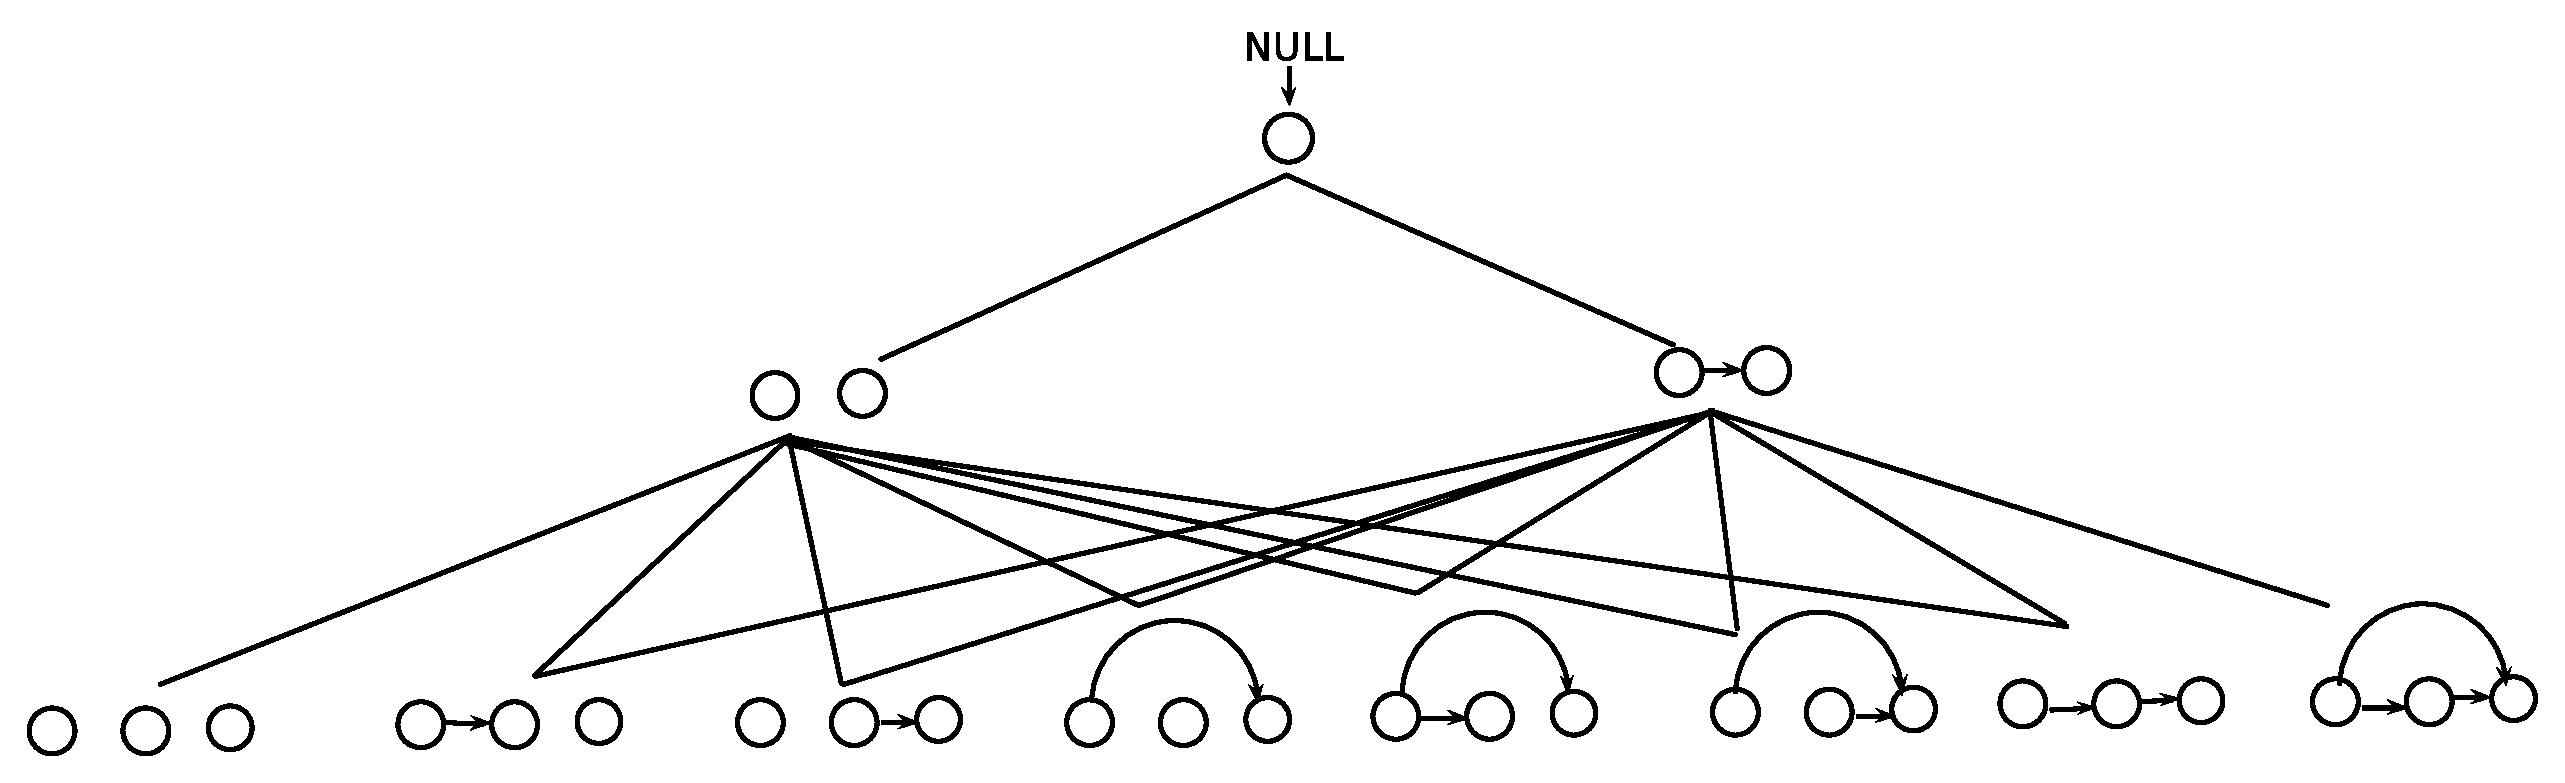
\includegraphics[scale=.38]{./figures/parent_child_relation.eps}
\caption{parent child relation.} 
\label{f:parent_child_rel}
\end{figure*}

Kneser-Ney smoothing uses a discount factor to discount the raw count
of each event (subgraph) and distributes the total discount to all
event (subgraph) probabilities by means of a base probability.

The estimated frequency of subgraph $sg$ in a given sentence graph
is computed as follows:

\begin{equation*}
KN(sg) = \frac{\max \lbrace	 count(sg)-\alpha, 0 \rbrace }{Z} + \frac{M \cdot \alpha}{Z}P_b(sg),
\end{equation*}
%
where $\alpha$ is the discount factor and $M$ is the number of times
that discount factor is applied. $Z$ is a normalization factor
to ensure that the distribution sums to one and is obtained as follows:

\begin{equation*}
Z = \sum_{sg \in A} count(sg),
\end{equation*}
%
where $A$ is the set of all subgraphs with \knodes\ and function
$count(\cdot)$ computes the number of instances of subgraph $sg$ in
the given sentence graph.

$P_b(sg)$ in Kneser-Ney smoothing is the base probability of
subgraph $sg$ among all \knode\ subgraphs ($A$). The base
probability can be computed based on hierarchical (parent-child)
relations in subgraphs. \knode\ subgraph $sg_i$ is a parent
of \kplusnode\ subgraph $sg_j$, if $sg_i$ is a subgraph of
$sg_j$. Figure \ref{f:parent_child_rel} shows the parent-child
relation between subgraphs via a weighted tree. The root of this tree
is a null graph
\footnote{A null graph is a graph with no nodes.}. 
The weight of a parent-child relation connecting the parent
subgraph $sg_i$ and child subgraph $sg_j$ is shown by $w_{ij}$ and
computed as follows:

\begin{equation*}
w_{ij} = \frac{count(sg_i, sg_j)}{\sum_{sg_l \in A}count(sg_i,sg_l)},
\end{equation*}
%
where $A$ is all subgraphs with \knode\ and $k$ equals the number of
nodes of $sg_j$. Interpretation of weight $w_{ij}$ is the normalized count of $sg_i$ in $sg_j$ with respect to all outgoing edges from $sg_i$.

The base probability of each subgraph $sg_j$ is the inner product
of the Kneser-Ney probabilities of $sg_j$'s parents by the weights of
the corresponding relations:

\begin{equation}
P_b(sg_j)  = P \cdot W,
\end{equation}
%
where $P$ is the vector of probabilities of all parents of 
$sg_j$ and $W$ is the vector of all corresponding edge weights
connecting the parents of $sg_j$ to $sg_j$.

Since the root node of this tree is the null subgraph, and it is a
subgraph of all possible sentence graphs, its base probability is
one. Because the edge weights are in the range $\left[0,1\right]$ the
sum of the probabilities of all subgraphs with \knode\ is always
equal to one.

\paragraph{Proof.} 
Assume $I$ and $J$ are the set of all \knode\ and \kplusnode\
subgraphs. We also assume that $I$ has $n$ subgraphs and $\sum_{i=1}^n
p(sg_i)=1$. Considering these assumptions we prove that

\begin{equation*}
\sum_{j=1}^m p(sg_j)=1,
\end{equation*}

\noindent
where $m$ is the number of subgraphs in $J$.

We start from the left and compute the value of 

\begin{equation*}
\sum_{j=1}^m p(sg_j).
\end{equation*}

\noindent
Based on the definition of base probability, the value of
$p(sg_j)$ is computed based on its parents in $I$,

\begin{equation*}
p(sg_j)=\sum_{i=1}^n w_{ij}p(sg_i),
\end{equation*}

\noindent
where $w_{ij}$ is the weight of the parent-child relation between
$sg_i$ and $sg_j$.  Now we have:

\begin{equation*}\sum_{j=1}^m p(sg_j) = \sum_{j=1}^m\sum_{i=1}^n w_{ij}p(sg_i).
\end{equation*}

\noindent
If we exchange the place of the sums and re-write the equation, we
have: 

\begin{equation*}
\sum_{j=1}^m p(sg_j) = \sum_{i=1}^n \sum_{j=1}^m w_{ij}p(sg_i).
\end{equation*}

\noindent
In this equation $p(sg_i)$ is independent of $j$ (index of the inner
sum), so it can be moved out of the inner sum:

\begin{equation*}
\sum_{j=1}^m p(sg_j) = \sum_{i=1}^n p(sg_i) \sum_{j=1}^m w_{ij}
\end{equation*}

\noindent
The inner sum equals $1$.

\begin{equation*}
\sum_{j=1}^m p(sg_j) = \sum_{i=1}^n p(sg_i).
\end{equation*}

\noindent
Based on our assumption the right side of the equation is $1$ and 

\begin{equation*}
\sum_{j=1}^m p(sg_j) = 1.
\end{equation*}

\noindent
So we proved that the sum of the base probability of all \knode\
subgraphs is $1$.\QEDB


This way, Kneser-Ney smoothing distributes the total discount value by
considering the weights of parent-child relations among the
subgraphs. The result of applying smoothing is an estimation of the
frequency of each subgraph in the sentence graph.



\section{Experiments}
\label{sec:experiments}

\footnote{We use threshold $0.9$. It means we capture the semantic connection confidentially}


\subsection{Readability Assessment}
\label{subsec:readability_assessment}
We evaluate our coherence model on the task of ranking texts by their
readability. The intuition is that more coherent texts are easier to
read. 


\subsubsection{Data}
\paragraph{Datasets.} We run our experiments on two datasets annotated
with readability information provided by human annotators: \emph{P\&N}\
\cite{pitler08} and \emph{De Clercq}\ \cite{declercq14}.

The dataset \emph{P\&N}\ contains 27 articles randomly selected from
the Wall Street Journal corpus%
%
\footnote{\newcite{pitler08}'s dataset contains 30 articles. They
  remove one. We assume this is \texttt{wsj\--0382} which
does not exist in the Penn Treebank. We furthermore remove
\texttt{wsj\--2090} which does not exist in the final release of the
Penn Discourse Treebank. We also remove \texttt{wsj\--1398} which is a
poem and, hence, not very informative for readability assessment.}%
%
. The average number of sentences is about $10$ words. Every article is
associated with a human score between $[0.0,5.0]$ indicating the
readability score of that article. We create pairs of documents, if
the difference between their readability scores is greater than
$0.5$. If the first document in a pair has the higher score, we label
this pair with $+1$, otherwise with $-1$. The resulting number of text pairs in
this dataset is $209$.

The dataset \emph{De Clercq}\ consists of $105$ articles from different
genres: administrative (17 articles), journalistic (43 articles), manuals (14 articles) and miscellaneous (31 articles). The
average number of sentences is about $12$. This dataset was annotated
by \newcite{declercq14} by asking human judges to compare two texts
based on their readability. They use five labels:
\squishlist
\item[\textbf{LME:}] left text is much easier,
\item[\textbf{LSE:}] left text is somewhat easier, 
\item[\textbf{ED:}] both texts are equally difficult,
\item[\textbf{RSE:}] right text is somewhat easier,
\item[\textbf{RME:}] right text is much easier.
\squishend

We map these labels to three class labels:

\squishlist
\item[\textbf{$+1$:}] for text pairs where the left text is easier to read
  (LME or LSE),
\item[\textbf{$0$:}] for text pairs where both texts are equally
  difficult to read (ED), 
\item[\textbf{$-1$:}] for text pairs where the right text is easier to read (RSE or RME).
\squishend

Properties of this dataset are shown in Table \ref{table:genre_prop}.

\begin{table}[!h]
\centering
\begin{tabular}{lcc}
\hline
Genre & No.\ of articles & No.\ of text pairs \\\hline
Administrative & 17 & 272 \\
Journalistic & 43 & 1806 \\
Manuals & 14 & 182 \\
Miscellaneous & 31 & 931\\\hline
\end{tabular}
\caption{Properties of the different genres in the \emph{De Clercq} dataset.}
\label{table:genre_prop}
\end{table}

\subsubsection{Settings}
\paragraph{Word Embeddings and Classification.} In order to reduce the
effect of very frequent words, stop words are filtered by using the
SMART English stop word list \cite{salton71}. We use a pre\-trained
model of GloVe for word embeddings. This model is trained on Common
Crawl with 840B tokens, 2.2M vocabulary. We represent each word by a
vector with length 300 \cite{pennington14}.  For handling
out-of-vocabulary words, we assign a random vector to each word and
memorize it for its next occurrence \cite{kusner15}. 
The classification task is done by the SVM implementation in WEKA (SMO)
with the linear kernel function. All settings are set to the default
values. The evaluation is computed by 10-fold cross validation.

\paragraph{Graph Processing and Smoothing.} In order to compare the
performance of LCG with the entity graph model, we follow
\newcite{mesgar15} and use the gSpan method \cite{yanxifeng02} to compute all common
subgraphs on each dataset and their frequencies. Note that gSpan
does not count all possible \knode\ subgraphs, whereas for applying
Kneser-Ney smoothing it is necessary to count all possible \knode\
subgraphs, because the probability should be distributed among all
possible subgraphs.  This also helps to estimate the probability of
unseen patterns. We use a random sampling method \cite{shervashidze09}
to obtain the frequency of subgraphs in a sentence graph. In this
regard, we take $10,000$ samples of the given sentence graph by
randomly selecting $k$ nodes of the graph to count the occurrence of
\knode\ subgraphs in this graph. We compute the base probability for
at most $k = 6$. We find the best value for $d$ in a greedy
manner. First, we initialize $d$ with $0.001$. In each iteration we
compute the performance. Then we multiply the discount factor by $10$. We
iterate as long as the discount factor is less than $1000$. We report
the best performance.

\subsubsection{Results}
In order to compare our method with related work, we run our model on
the \emph{P\&N}\ dataset. Table \ref{table:pitler} reports the accuracy
of \emph{LCG}\ with different values for $k$ in \knode\
subgraphs. This corresponds to coherence patterns spanning
different numbers of sentences.

\begin{table}[!h]
\centering
\begin{tabular}{lccc}
\hline
System & \multicolumn{3}{c}{Accuracy}\\
\hline
ZeroR & \multicolumn{3}{c}{50.24\%}\\
EGrid	&	\multicolumn{3}{c}{83.25\%}\\\hline
\knode\ & EGraph\hspace*{2mm} & EGraph+PRN\hspace*{2mm}	&  LCG \\\hline
3-node& 79.43\%\hspace*{4mm} & 80.38\%** 		&  78.95\% \\
4-node& 89.00\%\hspace*{4mm} & 89.95\%\hspace*{4mm} 		&  89.47\%  \\
5-node& 96.17\%** 			  & 95.69\%** 					&  97.13\%  \\\hline
\end{tabular}
\caption{\emph{P\&N} dataset.}
\label{table:pitler}
\end{table}


We start in Table \ref{table:pitler} with a majority class baseline
(\emph{ZeroR}). \emph{EGrid}\ is our reimplementation of
\newcite{pitler08} which we use as non-trivial baseline. The column
\emph{EGraph}\ is the entity graph model of \newcite{mesgar15}. In
\emph{EGraph+PRN}\ we extend this model by a pronoun resolution
system, so that entities mentioned by pronouns also enter the
graph. We apply the Stanford coreference resolution system
\cite{leeheeyoung13}. Using the full coreference resolution system,
however, decreases performance, hence we only use resolved
pronouns. The enriched model with resolved pronouns works slightly
better for \emph{3-node}\ and \emph{4-node}\ subgraphs, and slightly
worse for \emph{5-node}\ subgraphs than the \emph{EGraph}. The lexical
coherence graph model, \emph{LCG}, performs slightly worse than
\emph{EGraph}\ on \emph{3-node}\ subgraphs. This could be because the
graphs in \emph{LCG}\ have more edges than the graphs in
\emph{EGraph}. When graphs are denser \emph{3-node}\ subgraphs occur
in every graph, hence their frequency is less discriminative. As shown
in Table \ref{table:pitler} larger subgraphs (\emph{4-node}\ and
\emph{5-node}) capture more information and improve upon
\emph{EGraph}\ and for \emph{5-node}\ subgraphs even upon
\emph{EGraph+PRN}. \emph{LCG} significantly ($p\_value=0.01$) works
better than \emph{EGraph+PRN} and \emph{EGraph} using 5-node
subgraphs. The difference between \emph{LCG} and \emph{EGraph+PRN} and
\emph{EGraph} using 4-node subgraphs is not significant.

Table \ref{table:clercq} shows the performance of different models on
the \emph{De Clercq} dataset.  

\begin{table}[!h]
\centering
\begin{tabular}{lccc}
\hline
System & \multicolumn{2}{c}{Accuracy}\\
\hline
ZeroR	& \multicolumn{2}{c}{42.312\%}\\\hline
\knode\ & EGraph+PRN	& LCG\hspace*{2mm}  \\\hline

3-node & 42.31\% & 42.31\%\hspace*{4mm}	\\
4-node & 48.07\% & 49.12\%** \\
5-node & 65.77\% & 76.27\%**	\\\hline

\end{tabular}
\caption{\emph{De Clercq}\ dataset.}
\label{table:clercq}
\end{table}

Again, we use a majority baseline (\emph{ZeroR}) to put our results in context. While the performance of both methods almost does not beat the baseline for \emph{3-node}\ subgraphs, \emph{4-node}-subgraphs work already better, and \emph{5-node}\ subgraphs yield reasonable performance on this dataset. Although \emph{EGraph+PRN} and \emph{LCG} reach almost the same performance for \emph{4-node}, the difference between them is statistically significant ($p\_value=0.01$). With \emph{5-node} subgraphs, \emph{LCG} outperforms \emph{EGraph+PRN} subgraphs by a large margin and gets a very reasonable performance on this dataset.

The general performance on the \emph{De Clercq} dataset is lower
than the performance on the the \emph{P\&N} dataset. This can have two
reasons: first, the ranking task on the \emph{De Clercq} dataset is
three-label classification which is more difficult than the binary
classification task on the \emph{P\&N} dataset. Second, texts in the
\emph{De Clercq} dataset are from different genres and coherence patterns
may vary across genres. Hence, we take a closer look on the
performance on the different genres.

\begin{table}[!h]
\centering
\begin{tabular}{lccc}
\hline
\emph{5-node}\ & EGraph+PRN	& LCG \\\hline
Administrative	& 69.49\%	& 	71.69\%	\\
Journalistic	& 65.01\%	& 	82.12\%\\
Manuals 		& 54.95\% 	& 	61.54\%	\\
Misc.			& 70.68\%	& 	76.69\% \\\hline
\end{tabular}
\caption{Accuracy of \emph{EGraph+PRN}\ and \emph{LCG}\ on different
  genres in the \emph{De Clercq}\ dataset.}
\label{table:clercq_genre}
\end{table}

Table \ref{table:clercq_genre} shows the performance for
\emph{EGraph+PRN}\ and \emph{LCG}\ using \emph{5-node}\ subgraphs on
the different genres in the \emph{De Clercq}\ dataset. The performance of
\emph{LCG}\ is higher than \emph{EGraph+PRN}\ on all genres. 
Unlike \emph{EGraph+PRN}, \emph{LCG}\ gets the best performance on journalistic articles. The lowest performance of both models is obtained on manuals. On administrative articles, performance of \emph{LCG}\ is slightly better than \emph{EGraph+PRN}. On  miscellaneous articles \emph{LCG}\ performs better than \emph{EGraph+PRN}.

While large subgraphs are very informative for coherence modeling,
extracting large subgraphs ($k>4$) in relatively small datasets leads
to a data sparsity problem, as there are very many possible subgraphs
to be represented in a high dimensional vector space. Hence, many
possible subgraphs have low or even zero counts.  The problem for such
a vector is that each graph is only similar to itself and not to any other
graph. Hence, we observe a drop in performance when the model deals
with large subgraphs (\emph{6-node} subgraphs, \emph{LCG1}\ for
\emph{P\&N}\ in Table \ref{table:smoothing}). We solve this problem by
smoothing. 

In order to apply Kneser-Ney smoothing we use a sampling method to
create all possible (connected and disconnected) \knode\ subgraphs
(for \emph{LCG1}\ and \emph{LCG1*}\ we use connected and disconnected
subgraphs, for \emph{LCG}\ only connected ones).

Table \ref{table:smoothing} shows the performance of \emph{LCG1}\ when
it is applied to ever larger subgraphs. As can be seen in Table
\ref{table:smoothing}, the performance on the \emph{P\&N}\ dataset
suddenly drops for \emph{6-node}\ subgraphs. This is could be caused by the
sparsity problem.

\begin{table}[!h]
\centering
%\small
\begin{tabular}{@{}ccccc@{}}
\\\hline
 & \multicolumn{2}{@{}c}{\emph{P\&N}} & \multicolumn{2}{c@{}}{\emph{De Clercq}} \\\hline
\knode\ & LCG1 & LCG1* & LCG1 & LCG1* \\\hline
3-node & 84.52\% & 89.00\% & 42.31\% & 49.60\% \\
4-node & 95.69\% & 96.17\% & 65.10\% & 66.23\% \\
5-node & 97.61\% & 98.08\% & 79.33\% & 79.85\% \\
6-node & 93.26\% & 95.69\% & 76.67\% & 78.03\%\\\hline
\end{tabular}
\caption{Applying smoothing method yields to higher accuracy for larger subgraphs.}
\label{table:smoothing}
\end{table}

When we apply Kneser-Ney smoothing as described in Section
\ref{sec:method} the results for all tested values of $k$ are superior
for \emph{LCG1*}\ when compared to \emph{LCG1}\ (Table
\ref{table:smoothing}).

Kneser-Ney smoothing improves the performance of the system even with
\emph{3-node}\ subgraphs by a large margin. Smoothing reduces the
power of frequency and makes the frequency distribution of subgraphs
more even. Smoothing reduces the values through all
subgraphs by considering parent-child relations between subgraphs to
relate similar subgraphs. That is the advantage of the Kneser-Ney
method in comparison to the other smoothing methods like
Laplace-Smoothing. 

For the \emph{P\&N}\ dataset we achieve the best results to
date. \newcite{pitler08} reported 83.25\% accuracy, \newcite{mesgar15}
89.95\%. When smoothing \emph{5-node}\ subgraphs we are able to report
98.08\%. This, however, indicates that this dataset may not be the
best one to report performance on. Hence, we now check whether
smoothing also improves the performance on the more difficult
\emph{De Clercq}\ dataset.

On this dataset, we basically observe the same trends. Both settings result in better performance than \emph{LCG}\ (see Table \ref{table:clercq}). 

Note that none of the parameters in this work is tuned on the
datasets. One may get better performance by tuning the parameters.
The results confirm the intuition
that the lexical coherence graph \emph{LCG}\ captures coherence and
models lexical coherence appropriately.

Applying smoothing on graphs of \emph{EGraph+PRN} model increases the performance of this model. But this improvement is not as high as the improvement on the \emph{LCG} graph.

\paragraph{Coherence Patterns.}
In this part we check the Pearson correlation coefficient between
\emph{LCG1}\ and human judgements of a few frequent subgraphs on the
\emph{P\&N}\ dataset. In order to be consistent with
\newcite{mesgar15}, we use the exhaustive value of subgraph
frequencies, i.e.\ \emph{LCG1}\ for our work.

For the \emph{3-node}\ subgraphs only one subgraph (Figure
\ref{fig:correlated_graphs}) in the \emph{LCG1}\ representation is
significantly (and positively) correlated (\emph{p-value}$<0.05$) with
human scores. For the \emph{4-node}\ subgraphs, we find six subgraphs
which are significantly correlated with readability. Only one is
positively correlated, while four are negatively
correlated. Interestingly, both positively correlated \emph{3-node}\
and \emph{4-node}\ subgraphs have been determined as positively and
significantly correlated by \newcite{mesgar15} as well. Both also
capture a similar coherence pattern, indicating that our method is
linguistically sound.

\begin{figure}[!ht]
\centering
\small
%\begin{tabular}{lc|cc}
\hline
& Pattern & $\rho$ & p-value \\\hline
%%%%%%%%%%%%%%%%%%%%%%%%%%%%%%%%%%%%%%%%%%%%%%%%%%%%
\rb{\emph{3-node}} &
\begin{tikzpicture}[shorten >=1pt,->,scale=0.5]  
        \tikzstyle{sentence}=[circle,thick,draw=black!75,fill=black!10,minimum size=2mm]
        \tikzstyle{edge}=[draw, thick]
       \begin{scope}
         \node [sentence] (s1) at (0,2) {\tiny{}};
         \node [sentence] (s2) at (2,2) {\tiny{}};
         \node [sentence] (s3) at (1,0) {\tiny{}}; 
         \path[edge] (s1) edge [above] node[font=\tiny] {} (s2);
         \path[edge] (s1) edge [above] node[font=\tiny] {} (s3);
        \end{scope}        
\end{tikzpicture}
      &	\rb{0.43} & \rb{0.024}
      \\\hline
\rb{\emph{4-node}} &
\begin{tikzpicture}[shorten >=1pt,->,scale=0.5]  
        \tikzstyle{sentence}=[circle,thick,draw=black!75,fill=black!10,minimum size=1mm]
        \tikzstyle{edge}=[draw, thick]
       \begin{scope}
         \node [sentence] (s1) at (0,2) {\tiny{}};
         \node [sentence] (s2) at (2,2) {\tiny{}};
         \node [sentence] (s3) at (2,0) {\tiny{}};
         \node [sentence] (s4) at (0,0) {\tiny{}};  
         \path[edge] (s1) edge [above] node[font=\tiny] {} (s3);
         \path[edge] (s1) edge [above] node[font=\tiny] {} (s4);
         \path[edge] (s2) edge [above] node[font=\tiny] {} (s3);
         \path[edge] (s3) edge [above] node[font=\tiny] {} (s4);
        \end{scope}        
      \end{tikzpicture}
      &	\rb{-0.45} & \rb{0.018}
      
       \\
&
\begin{tikzpicture}[shorten >=1pt,->,scale=0.5]  
        \tikzstyle{sentence}=[circle,thick,draw=black!75,fill=black!10,minimum size=1mm]
        \tikzstyle{edge}=[draw, thick]
       \begin{scope}
         \node [sentence] (s1) at (0,2) {\tiny{}};
         \node [sentence] (s2) at (2,2) {\tiny{}};
         \node [sentence] (s3) at (2,0) {\tiny{}};
         \node [sentence] (s4) at (0,0) {\tiny{}};  
         \path[edge] (s1) edge [above] node[font=\tiny] {} (s2);
         \path[edge] (s1) edge [above] node[font=\tiny] {} (s3);
         \path[edge] (s1) edge [above] node[font=\tiny] {} (s4);
         \path[edge] (s2) edge [above] node[font=\tiny] {} (s3);
        \end{scope}        
      \end{tikzpicture}
      &	\rb{+0.39} & \rb{0.047}
      \\
&
      \begin{tikzpicture}[shorten >=1pt,->,scale=0.5]  
        \tikzstyle{sentence}=[circle,thick,draw=black!75,fill=black!10,minimum size=1mm]
        \tikzstyle{edge}=[draw, thick]
       \begin{scope}
         \node [sentence] (s1) at (0,2) {\tiny{}};
         \node [sentence] (s2) at (2,2) {\tiny{}};
         \node [sentence] (s3) at (2,0) {\tiny{}};
         \node [sentence] (s4) at (0,0) {\tiny{}};  
         \path[edge] (s1) edge [above] node[font=\tiny] {} (s4);
         \path[edge] (s2) edge [above] node[font=\tiny] {} (s3);
         \path[edge] (s3) edge [above] node[font=\tiny] {} (s4);
        \end{scope}        
      \end{tikzpicture}
      &	 \rb{-0.43}  & \rb{0.024}
      \\
&
      \begin{tikzpicture}[shorten >=1pt,->,scale=0.5]  
        \tikzstyle{sentence}=[circle,thick,draw=black!75,fill=black!10,minimum size=1mm]
        \tikzstyle{edge}=[draw, thick]
       \begin{scope}
         \node [sentence] (s1) at (0,2) {\tiny{}};
         \node [sentence] (s2) at (2,2) {\tiny{}};
         \node [sentence] (s3) at (2,0) {\tiny{}};
         \node [sentence] (s4) at (0,0) {\tiny{}};  
         \path[edge] (s1) edge [above] node[font=\tiny] {} (s3);
         \path[edge] (s2) edge [above] node[font=\tiny] {} (s3);
         \path[edge] (s3) edge [above] node[font=\tiny] {} (s4);
        \end{scope}        
      \end{tikzpicture}
      &	\rb{-0.59} & \rb{0.001}
      \\
&
      \begin{tikzpicture}[shorten >=1pt,->,scale=0.5]  
        \tikzstyle{sentence}=[circle,thick,draw=black!75,fill=black!10,minimum size=1mm]
        \tikzstyle{edge}=[draw, thick]
       \begin{scope}
         \node [sentence] (s1) at (0,2) {\tiny{}};
         \node [sentence] (s2) at (2,2) {\tiny{}};
         \node [sentence] (s3) at (2,0) {\tiny{}};
         \node [sentence] (s4) at (0,0) {\tiny{}};  
         \path[edge] (s1) edge [above] node[font=\tiny] {} (s2);
         \path[edge] (s2) edge [above] node[font=\tiny] {} (s4);
         \path[edge] (s3) edge [above] node[font=\tiny] {} (s4);
        \end{scope}        
      \end{tikzpicture}
      &	\rb{-0.55} & \rb{0.003}
      \\
&
      \begin{tikzpicture}[shorten >=1pt,->,scale=0.5]  
        \tikzstyle{sentence}=[circle,thick,draw=black!75,fill=black!10,minimum size=1mm]
        \tikzstyle{edge}=[draw, thick]
       \begin{scope}
         \node [sentence] (s1) at (0,2) {\tiny{}};
         \node [sentence] (s2) at (2,2) {\tiny{}};
         \node [sentence] (s3) at (2,0) {\tiny{}};
         \node [sentence] (s4) at (0,0) {\tiny{}};  
         \path[edge] (s1) edge [above] node[font=\tiny] {} (s2);
         \path[edge] (s2) edge [above] node[font=\tiny] {} (s3);
         \path[edge] (s2) edge [above] node[font=\tiny] {} (s4);
        \end{scope}        
      \end{tikzpicture}
      &	\rb{-0.55} & \rb{0.003}
      
\end{tabular}


\caption{Pearson correlation between \emph{3-node}\ and \emph{4-node}\
  subgraphs and readability scores in the \emph{P\&N}\ dataset.}
\label{fig:correlated_graphs}
\end{figure}

\section{Related Work}
\label{sec:lcg_	related_work}
The entity grid model \cite{barzilay08} is based on entity transitions
over sentences. It uses a two dimensional matrix to represent
transitions of entities among adjacent sentences. The entity grid is
applied to readability assessment by \newcite{pitler08}. The entity
graph \cite{guinaudeau13} is a graph-based, mainly unsupervised
interpretation of the entity grid. This model represents the
distribution of entities over sentences in a text with a bipartite
graph. Connections between sentences are obtained by information on
entites shared by sentences. \newcite{guinaudeau13} perform a one-mode
projection on sentence nodes and use the average out-degree of
the one-mode projection graph to quantify the coherence of the given
text. \newcite{mesgar15} represent the connectivity of the one-mode
projection graph by a vector whose elements are the frequencies of
subgraphs in projection graphs. This encoding works much better
than the entity graph for the readability task on the \emph{P\&N}
dataset and even outperforms \newcite{pitler08} by a large margin.
\newcite{zhangmuyu15} state that the entity graph model is limited,
because it only captures mentions which refer to the same entity (the
entity graph uses a very restricted version of coreference resolution
to determine entities). \newcite{zhangmuyu15} use world knowledge
\emph{YAGO} \cite{hoffart13}, \emph{WikiPedia} \cite{denoyer06} and
\emph{FreeBase} \cite{bollacker08} to capture the semantic relatedness
between entities even if they do not refer to the same entity. Main
issues with using world knowledge are: the choice knowledge sources, selection of knowledge from the source, coverage, and language-dependence.

Word embedding approaches like \emph{word2vec}\ and \emph{GloVe}\
\cite{mikolov13c,pennington14} show that the semantic connection
between words can be captured by word vectors which are obtained by
applying a neural network. The ability to train on very
large data sets allows the model to learn complex relationships
between words.

The entity grid model \cite{barzilay08} is based on entity transitions
over sentences. It uses a two dimensional matrix to represent
transitions of entities among adjacent sentences. The entity grid is
applied to readability assessment by \newcite{pitler08}. The entity
graph \cite{guinaudeau13} is a graph-based, mainly unsupervised
interpretation of the entity grid. This model represents the
distribution of entities over sentences in a text with a bipartite
graph. Connections between sentences are obtained by information on
entites shared by sentences. \newcite{guinaudeau13} perform a one-mode
projection on sentence nodes and use the average out-degree of
the one-mode projection graph to quantify the coherence of the given
text. \newcite{mesgar15} represent the connectivity of the one-mode
projection graph by a vector whose elements are the frequencies of
subgraphs in projection graphs. This encoding works much better
than the entity graph for the readability task on the \emph{P\&N}
dataset and even outperforms \newcite{pitler08} by a large margin.
\newcite{zhangmuyu15} state that the entity graph model is limited,
because it only captures mentions which refer to the same entity (the
entity graph uses a very restricted version of coreference resolution
to determine entities). \newcite{zhangmuyu15} use world knowledge
\emph{YAGO} \cite{hoffart13}, \emph{WikiPedia} \cite{denoyer06} and
\emph{FreeBase} \cite{bollacker08} to capture the semantic relatedness
between entities even if they do not refer to the same entity. Main
issues with using world knowledge are: the choice knowledge sources, selection of knowledge from the source, coverage, and language-dependence.

Word embedding approaches like \emph{word2vec}\ and \emph{GloVe}\
\cite{mikolov13c,pennington14} show that the semantic connection
between words can be captured by word vectors which are obtained by
applying a neural network. The ability to train on very
large data sets allows the model to learn complex relationships
between words.


\section{Conclusions}
\label{sec:lcg_conclusion}
%
In this paper we propose a new graph based coherence model, the
lexical coherence graph, LCG. We view coherence as semantic
connectedness between words which we model by word embeddings. We take
only the strongest connection between sentences to create a graph with
connected sentences. Then we extract large subgraphs capturing
coherence patterns, which show similarity to patterns described in
text linguistics \cite{danes74a}.

While the entity grid works only on sequences of up to three adjacent
sentences, we are able to model relationships of up to six
non-adjacent sentences. We solve the sparsity problem of large
subgraphs by adapting Kneser-Ney smoothing to graphs. Smoothing
prevents LCG from losing performance with large subgraphs and leads to
superior performance on the \newcite{pitler08} dataset and to a
first reasonable state-of-the-art on the \newcite{declercq14} dataset.

In future work we want to apply LCG to essay scoring as well. Also, we
see that our adaption of Kneser-Ney smoothing to graphs may be useful
for research in subgraph mining in general.

In this paper, we employed the graph-based representation of local coherence by \newcite{Mesgar2016} 
for the machine translation task by integrating the graph-based coherence features with the document-level MT decoder Docent \cite{Hardmeier2012a, Hardmeier2013a}. 
The usage of these coherence features has been shown for readability assessment and multi-document summarization \cite{Parveen2016,Mesgar2016}. We are the first who utilize these coherence features for document-level translation.
Our coherence model using subgraph frequencies  as coherence features improves the performance of Docent as a document-level MT decoder.
For future work, we are going to check if the connectivity structure of the source document can help the translation system to improve the translation quality of each sentence. This idea is inspired from the application of topic-based coherence modeling in machine translation before \cite{Xiong2013}.


\newcite{hoey91}'s argument is that lexical cohesion is the most important of all cohesion-creating devices in texts. 
Thus, if some textual areas contain no lexical relations, we are dealing with marginal sentences and the ideas expressed through these sentences should generally not be included in a summary. 
\newcite{stotesbury93} categorize lexical relations as follows:
\begin{itemize}
\item Simple lexical repetition: which means lexical items appear in an identical form e.g., debate (sg.) - debates (pl.)
\item Complex repetition: covers the cases sharing a lexical morpheme (e.g. history - historian); antonym formed by affixes (e.g. significant- insignificant)
\item Simple lexical paraphrase: this can be mutual or partial. 
Partial paraphrase would be for example reference made by a paraphrase, historian, to a person whose name was mentioned earlier. 
\item Complex paraphrase: this covers three different cases: 
\begin{itemize}
    \item antonyms that are not formed with affixes (e.g. willing - reluctant)
    \item the link triangle comes into play when there are two repetitive links already identified. 
    For example the relation between history and historian, and historian is related to scholar. 
    The third case occurs when one of the two links is missing but could imagine to exist in a particular context. 
\end{itemize} 
\end{itemize}

\newcite{stotesbury93} represent the lexical repetitions in a text as a matrix whose rows and columns are sentence IDs and entries are the number of lexical connections between their corresponding sentences. 
They also use a threshold to recognize the connection between sentences. 
If a sentence is connected to less than three other sentence, its connections are discarded \cite{stotesbury93}. 
The last step in \newcite{stotesbury93} is removing unwanted cohesion in a summary. 
In addition, if some sentences are not coherence or mutually relevant, they can and should be deleted from the summary. 
They compare the automatic summary produced by their systems with a human generated summary. 
They conclude that their summarizer that is mainly based on the lexical connections contain important sentences and therefore important information. 
Hoey's expectation of the efficiency of his methodology is that "it might be possible to use central sentences to produce a readable summary of the text or to trace themes through the text by using all the sentences that link with a particular sentence."
Hoey's argument is that ``relevance is in part a function of multiple repetition" and ``our understanding of texts in part deponds on our ability to make connections across text on the same factor of multiple repetitions."
 \newcite{stotesbury93} conclude that the result of their analysis show that adjacent sentences do not share many words very often in mature English writing. 
 Therefor the old advice to avoid repetition still holds in principle. 
 However, they advice that instead of avoiding repetition, they should be use to make connections across texts rather than between previous or subsequent sentences. 


 Discourse is more than a random set of sentences: it shows connectedness. 
 Coherence models are about characterizing this connectedness.

 The basis of lexical cohesion is in fact extended to any pair of lexical items that stand next to each other in some recognizable lexicosemantic relation \cite{sandres06} % paper is in linguistic collections cohesion and coherence: linguistic approaches

 The clearest case of lexical cohesion are those in which a lexical item is replaced by another item that is systematically related to the first one. 
 The notion of lexical cohesion is hard to define, especially when we need to find elements of sentences that are semantically related. 
 However, they argue that cohesion is not necessary for connectedness. 
 The dominant view is that the connectedness of a text is the characteristic of the mental representation of the text rather than of the text itself. 
Language users establish coherence by actively relating the different information units in the text. 
Coherence is a multilevel phenomenon, so that two segments may be simultaneously related on different levels \cite{sandres06}.
The connectedness of spoken discourse is established by many other means than the ones discussed for written/monolingual texts. 
Aspects of discourse that are specific to spoken language include the occurrence of adjacent pairs, i.e., minimal pairs Question-Answers. 
In sum, while cohesion seeks the answer in overt textual signals, a coherence approach considers connectedness to be of a cognitive nature.     



% % for sublime text 3
%!TEX root = diss.tex

\chapter{Related Work}
\label{ch:rel-work}
 
The task of coherence modeling has received a lot of attention due to its key impact in other natural language processing systems. 
In this thesis, we propose a novel approach to local coherence modeling based on graph representations of texts. 
We apply our approach to two types of graphs.  
The first type captures coreferent relations between named entity mentions in a text.
The second one represents lexical relations among words in a text.  
Our coherence model is evaluated with respect to its impact on readability assessment and text summarization. 

Accordingly, we first review entity-based approaches to local coherence (Section \ref{sec:rel-entity-models}). 
We then survey lexical approaches (Section \ref{sec:rel-ent-grid}). 
Finally, we discuss applications for local coherence model that have been introduced in the literature, particularly readability assessment and summarization tasks (Section \ref{sec:rel-coh-applications}). 
% A coherent text consists of a sequence of topics in a structured way \cite{marcu97b,hearst97,gallery03}. 
% Related models are often constructed as sequential topical models. 
% Topics are modeled by a language model \cite{blei01} or Bayesian topic models \cite{eisenstein08}.
% For modeling the temporal structure, early research uses a Hidden Markov Model \cite{barzilay04}, and  
% later research employs sequential neural networks \cite{}. 

\section{Entity-Based Approaches to Local Coherence}
\label{sec:rel-entity-models}

The primary steps of the research presented in this thesis are inspired by entity-based models. 
In this section, we explain details of two popular entity-based coherence models: the entity grid model, and the entity graph model. 
We also briefly discuss their extensions.  

\paragraph{Historical Review.} Entity-based approaches to local coherence have a long history within the linguistic literature \cite{kuno72,halliday76,prince81a,joshi98}.
Most approaches are common in the primary assumption that coherence is perceived with respect to how entities are introduced and discussed in a text. 
Texts that keep referring to similar entities are supposed to be more coherent than those with random and unexpected switches from one entity to another. 
This premise is supported by different theories, one of which is Centering Theory \cite{grosz95,joshi98} (see Chapter \ref{ch:coherence}). 

A great deal of research has been devoted to directly implement Centering Theory \cite{miltsakaki00,karamanis04a}. 
This is challenging because a computational model needs to determine how to instantiate parameters of the theory that are often underspecified. 
Interestingly, \newcite{poesio04b} note that even for basic parameters of Centering Theory such as ``utterance'', ``realization'', and ``ranking'' (see Chapter \ref{ch:coherence} for their definitions), multiple interpretations have been developed, because in the original theory of centering these concepts are not explicitly specified. 
As an instance, in some papers entities are ranked with respect to the grammatical function \cite{brennan87,grosz95} of entity occurrences in a text, and in some other papers those are ranked with respect to the position of entity mentions in sentences \cite{prince81a}, the familiarity status, or the thematic role \cite{strube.cl99,moens08}.
As a result, two instantiations of the same theory make different predictions for the same input.  

Some studies try to avoid this by finding an instantiation of parameters which is most consistent with observable data \cite{strube.cl99,karamanis04a,poesio04b}. 
Some others adopt a specific instantiation so that the performance of the coherence model improves for a specific task. 
For example, \newcite{miltsakaki00} annotate a corpus of student essays with entity transition information, and then show that the distribution of transitions correlates with human grades. 
Analogously, \newcite{hasler03} investigate whether the centering theory can be used in evaluating the readability of text by annotating summaries produced by humans or machines with the entity transition information. 
To sum up, \newcite{poesio04b} demonstrate that the predictive power of the models that directly implement centering theory is highly sensitive to their parameter instantiations.  

\newcite{barzilay05a,barzilay08} propose a general framework for coherence modeling.  
The main goal of this framework is to eliminate the need to human annotations for parameters in the centering theory, regardless of what the evaluation task is. 
By some inspirations from the theory, this model hypothesizes that the distribution of entities in coherent texts reveal certain regularities that make these texts recognizable from incoherent ones. 
These regularities can be learned by machine learning approaches.  
Since this model has been the core of many research in the area of coherence modeling (including the research presented in this thesis), we explain details of this model.    

\subsection{The Entity Grid Model}
\label{sec:rel-ent-grid} 

\newcite{barzilay05a,barzilay08} are the first researchers who proposed a general  computational approach to local coherence modeling based on the entity relations across adjacent sentences.  
Supported by some linguistic work such as Centering Theory \cite{grosz95} and other entity-based theories of discourse \cite{prince81a}, they assume that the distribution of entities in coherent texts exhibits certain regularities that can be reflected in a grid topology, which is called the entity grid. 
In this thesis we refer to this model as the \emph{entity grid} model, because its key idea is to represent the distribution of entities (see Chapter \ref{ch:coherence} for definition of entities) across sentences in a text by a grid.   
In practice, mentions of an entity are linked together in order to show that they are referring to the same entity. 
Connections between mentions not only show that those are referring to the same entity, but also indicate that sentences that contain those mentions are (almost) about the same topic or information \cite{barzilay08}. 

\subsubsection{Text Representation: Entity Grid}

In this model each text is represented by a grid, which is a two dimensional array whose rows correspond to entities, and columns are matching to sentences.
An entry $r_{i;j}$ in a grid describes the syntactic role of entity $i$ in sentence $j$ if the entity is mentioned in the sentence. 
The syntactic roles are categorized as subject (S), object (O), or all other syntactic roles (X). 
In addition, if an entity is not mentioned in a sentence, a special marker (-) fills the corresponding entry $r_{i;j}$. 
Finally, if a sentence contains several mentions of one entity, their corresponding entry describes the most important grammatical role of the mentions: subject if possible, then object, or finally other. 

The discussion of the grid develops around the important question of which textual units are to be considered mentions of an entities, and how different mentions are to be linked to represent an entity. 
A perfect solution in this regard would use coreference resolution to recognize mentions, noun phrases, and link arbitrary mentions to the same entities and discarding noun phrases which do not correspond to an entity. 
Since coreference resolution systems are far from prefect\footnote{The highest reported precision of a coreference system on the ? dataset is ?.}, and tend to work even more poorly on incoherent texts, this approach is not generally one utilized.  
Moreover, a non-perfect general coreference system introduces more noise to a coherence model than what it fixes \cite{barzilay08}.  
As an alternative, implementations of the entity grid model tend to employ all noun phrases as mentions and perform a heuristic, but strict and simple, coreference resolution. 
They connect all mentions that have an identical head noun as one entity. 
Detailed discussions of this heuristic are given in \newcite{poesio04c} and \newcite{elsner10}. 

As an example consider the sample text\footnote{The text with ID D31010, taken from Document Understanding Conference (DUC-?) dataset, which we use in one of our experiments. Numbers are not marked because they are filtered out in preprocessing.} in Example \ref{ex:rel-text}. 
In this example, noun phrases are marked with brackets as an indication of mentions. 
Mentions in a sentence are associated with their syntactic functions in the sentence, noted with a letter (S: subject, O: object, and X: others) next to the brackets. 
%/hits/fast/nlp/mesgarmn/Data/ACL13/SummaryCoherence/texts/
%D31010.M.100.T.E.txt. Nubembers (e.g. 29) are filtered out in preprocessing.}  

\begin{examples}
\label{ex:rel-text}
\begin{tabular}{l@{\space}p{12.5cm}}
 $s_0$: &[An arctic cold wave]\textbf{\textsubscript{S}}, [the worst]\textbf{\textsubscript{X}} in [10 years]\textbf{\textsubscript{X}}, hit [parts]\textbf{\textsubscript{O}} of [Europe]\textbf{\textsubscript{X}}, bringing [sub-zero temperatures]\textbf{\textsubscript{O}} and killing [scores]\textbf{\textsubscript{O}} of [people]\textbf{\textsubscript{X}}. \\

 $s_1$: & Hardest hit were [Poland]\textbf{\textsubscript{S}}, [Bulgaria]\textbf{\textsubscript{S}}, and [Romania]\textbf{\textsubscript{S}} as well as [parts]\textbf{\textsubscript{S}} of [central]\textbf{\textsubscript{X}} and [eastern France]\textbf{\textsubscript{X}}. \\

$s_2$: &In [Poland]\textbf{\textsubscript{X}}, [three weeks]\textbf{\textsubscript{X}} of [sub-zero temperatures]\textbf{\textsubscript{X}} killed [at least 85 people]\textbf{\textsubscript{O}} in [November]\textbf{\textsubscript{X}}, 29 more than in [all]\textbf{\textsubscript{X}} of [the previous winter]\textbf{\textsubscript{S}}. \\


$s_3$: &[Most]\textbf{\textsubscript{S}} of [the victims]\textbf{\textsubscript{X}} were homeless [whose deaths]\textbf{\textsubscript{X}} by [exposure]\textbf{\textsubscript{X}} were alcohol related. \\

$s_4$: &[Blizzards]\textbf{\textsubscript{X}} and [cold temperatures]\textbf{\textsubscript{S}} also hit [Bulgaria]\textbf{\textsubscript{X}} and [Romania]\textbf{\textsubscript{O}}, stranding [hundreds]\textbf{\textsubscript{O}} in [their cars]\textbf{\textsubscript{X}}. \\

$s_5$: &Elsewhere, [snow]\textbf{\textsubscript{S}} blanketed [the Italian island]\textbf{\textsubscript{O}} of [Capri]\textbf{\textsubscript{X}} for [the first time]\textbf{\textsubscript{X}} in [10 years]\textbf{\textsubscript{X}}. 
\end{tabular}
\end{examples}
%%(ROOT (S (NP (NP (DT An) (JJ arctic) (JJ cold) (NN wave)) (, ,) (NP (NP (DT the) (JJS worst)) (PP (IN in) (NP (CD 10) (NNS years)))) (, ,)) (VP (VBD hit) (NP (NP (NNS parts)) (PP (IN of) (NP (NNP Europe)))) (, ,) (S (VP (VP (VBG bringing) (NP (JJ sub-zero) (NNS temperatures))) (CC and) (VP (VBG killing) (NP (NP (NNS scores)) (PP (IN of) (NP (NNS people)))))))) (. .)))

%%(ROOT (S (S (VP (ADVP (RBS Hardest)) (VBN hit))) (VP (VBD were) (NP (NP (NP (NNP Poland)) (, ,) (NP (NNP Bulgaria)) (, ,) (CC and) (NP (NNP Romania))) (CONJP (RB as) (RB well) (IN as)) (NP (NP (NNS parts)) (PP (IN of) (NP (NP (JJ central)) (CC and) (NP (JJ eastern) (NNP France))))))) (. .)))

%%(ROOT (S (PP (IN In) (NP (NNP Poland))) (, ,) (NP (NP (CD three) (NNS weeks)) (PP (IN of) (NP (JJ sub-zero) (NNS temperatures)))) (VP (VBD killed) (NP (QP (IN at) (JJS least) (CD 85)) (NNS people)) (PP (IN in) (NP (NNP November))) (, ,) (PP (ADVP (NP (CD 29)) (RBR more)) (IN than) (IN in) (NP (NP (DT all)) (PP (IN of) (NP (DT the) (JJ previous) (NN winter)))))) (. .)))

%%(ROOT (S (NP (NP (JJS Most)) (PP (IN of) (NP (DT the) (NNS victims)))) (VP (VBD were) (ADJP (JJ homeless) (SBAR (WHNP (NP (WP$ whose) (NNS deaths)) (PP (IN by) (NP (NN exposure)))) (S (VP (VBD were) (ADJP (RB alcohol) (VBN related))))))) (. .)))

%%(ROOT (S (NP (NP (NNS Blizzards)) (CC and) (NP (JJ cold) (NNS temperatures))) (ADVP (RB also)) (VP (VBD hit) (NP (NNP Bulgaria) (CC and) (NNP Romania)) (, ,) (S (VP (VBG stranding) (NP (NNS hundreds)) (PP (IN in) (NP (PRP$ their) (NNS cars)))))) (. .)))

%%(ROOT (S (ADVP (RB Elsewhere)) (, ,) (NP (NN snow)) (VP (VBD blanketed) (NP (NP (DT the) (JJ Italian) (NN island)) (PP (IN of) (NP (NNP Capri)))) (PP (IN for) (NP (NP (DT the) (JJ first) (NN time)) (PP (IN in) (NP (CD 10) (NNS years)))))) (. .)))
%%

The corresponding entity grid for the text that is shown in Example \ref{ex:rel-text} is presented in Table \ref{tab:rel-egrid}. 
In this grid we follow \newcite{barzilay05a, barzilay08} and consider head nouns of noun phrases to represent the named entities that they are referring to. 
The coreferent mentions are detected by string match over head nouns. 

\begin{table}[!ht]	
	\begin{center}
		\begin{tabular}{lcccccc}
			\hline
			WAVE 			& S & - & - & - & - & - \\
			WORST 			& X & - & - & - & - & - \\
			YEARS 			& X & - & - & - & - & X \\
			PARTS 			& O & O & - & - & - & - \\
			EUROPE  		& X & - & - & - & - & - \\
			TEMPERATURES  	& O & - & X & - & S & - \\
			SCORES  		& O & - & - & - & - & - \\
			PEOPLE  		& X & - & O & - & - & - \\
			POLAND 			& - & O & X & - & - & - \\
			BULGARIA  		& - & X & - & - & - & - \\
			ROMANIA  		& - & X & - & - & O & - \\
			CENTRAL  		& - & X & - & - & - & - \\
			FRANCE  		& - & X & - & - & - & - \\
			NOVEMBER  		& - & - & X & - & - & - \\
			WEEKS 			& - & - & S & - & - & - \\
			ALL 			& - & - & X & - & - & - \\
			WINTER  		& - & - & X & - & - & - \\
			MOST 			& - & - & - & S & - & - \\
			VICTIMS  		& - & - & - & X & - & - \\
			DEATHS 			& - & - & - & X & - & - \\
			EXPOSURE  		& - & - & - & X & - & - \\
			BLIZZARDS  		& - & - & - & - & S & - \\
			HUNDREDS  		& - & - & - & - & O & - \\
			CARS  			& - & - & - & - & X & - \\
			TIME  			& - & - & - & - & - & X \\
			SNOW  			& - & - & - & - & - & S \\
			ISLAND 			& - & - & - & - & - & O \\
			CAPRI 			& - & - & - & - & - & X \\
			\hline
		\end{tabular}
		\caption{The entity grid representation of the text presented in Example \ref{ex:rel-text}. The rows represent entities and columns encode sentences. 
		If an entity is mentioned in a sentence, their corresponding entry in the gird indicates the grammatical role of the mention in the sentence, otherwise the entry is marked by ``--''.} 
		\label{tab:rel-egrid}
	\end{center}
\end{table}

It is worth noting that although entities in the original version of the entity grid are indicated by the head of a noun phrase (such as \emph{flight} in Example \ref{ex:rel-text}), \newcite{elsner11a} show that adding non-head nouns (like "the personal \textbf{country} flight" in Example \ref{ex:rel-text}) to a grid is beneficial to improve the representation power of the entity grid model. 
This enables the model to involve both head nouns and pre-modifiers in noun phrases to link sentences. 
Therefore, \newcite{elsner11a} consider all nouns (both \emph{country},\emph{flight} in the above example) in their entity grid representation.  
The non-head mentions are given the role X. 

\subsection{Pattern Definition: Grammatical Transitions}
%
The key hypothesis in the entity grid model is that the way that entities are distributed and that grammatical roles of entity occurrences change through a text reveal similar patterns in coherent texts.  
\newcite{barzilay05a,barzilay08} predefine all possible transitions that may occur for an entity in a text. 

More concretely, they define a transition pattern as a sequence of employed symbols with size $n$, $\{ S,O,X,\textit{--} \}^n$. 
Each pattern represents both entity occurrences between sentences, and the way that their syntactic roles in $n$ adjacent sentences are changing. 
For instance, for two adjacent sentences ($n=2$) there are $16$ possible patterns, which are shown in Table \ref{table:rel-egrid-pattern}.

\begin{table}[!ht]
	\begin{center}
		\resizebox{\columnwidth}{!}
		{%
			\begin{tabular}{@{}cccccccccccccccc@{}}
			\hline
			S S & S O & S X & S -- & 
			O S & O O & O X & O -- & 
			X S & X O & X X & X -- & 
			-- S & -- O & -- X & -- -- 
			\\\hline
			\end{tabular}
		}%
	\end{center}
	\caption{Patterns that are defined in the entity grid model.  
	They represent all possible entity occurrences in two adjacent sentences. 
	Symbols S (subject), O (object), and X (other) show grammatical role of an entity in a sentence. Symbol ``--'' encodes that an entity is not mentioned in a sentence.}
	\label{table:rel-egrid-pattern}
\end{table}

Each pattern that is shown in Table \ref{table:rel-egrid-pattern} represents one possible way that an entity may occur in two adjacent sentences. 
For example, pattern ``S O'' encodes that an entity appears in two adjacent sentences, and its syntactic role is changing from subject to object in sentences. 
As another example, consider pattern ``S --''. 
It indicates that an entity is referred to by a mention in the subject position of a sentence, but the entity has no mention in the immediately next sentence. 

\subsubsection{Coherence Representation: Probabilities of Transitions}
%
The entity grid model revolves around this assumption that coherent texts reveal certain regularities over the frequency of transitions or patterns \cite{barzilay05a,barzilay08}.    
The frequency of patterns can be used as an indicator to the preference of coherent texts in using or avoiding certain transitions. 
However, in order to prevent the model to be biased towards the text length, a probability for each pattern is computed, rather than the frequency. 	 
More formally, given the entity grid representation of a text, the probability of occurring a transition pattern in the grid is computed as follows:

\begin{equation}
p(t) = \frac{n(t)}{n(t^*)},
\end{equation}
where $t$ is a transition, $n(t)$ indicates the number of times that transition $t$ is occurring in the entity grid, and denominator $n(t^*)$ depicts the number of occurrences of all patterns whose length is as same as the length of $t$ in the grid. 
For instance consider the grid in Table \ref{tab:rel-egrid}, the probability of pattern ``O O'' is .01, which is computed as a ratio of its frequency, i.e. one, divided by the total number of patterns of length two, i.e., 140. 

\textbf{CHECK IF THIS GRID MATCHES WITH WHAT CAMILE GAVE YOU. IF NOT, YOU SHOULD SAY THAT THIS GRID, INCLUDING SYNTACTIC ROLES AND HEAD NOUN FINDERS, IS GENERATED BY BROWNCOHERENCE TOOLKIT. 
HOW IS IT POSSIBLE THAT A SENTENCE DOES NOT HAVE ANY SUBJECT, SEE S2}   

Each text can thus be viewed as a distribution defined over patterns. 
Therefore, the entity grid model represent the coherence property of a text by a fixed set of pattern sequences using a standard feature vector notation, where each feature is the probability of its corresponding pattern in the grid representation of the text.  
Table \ref{tab:rel-egrid-probs} shows the feature vector representation of the gird presented in Table \ref{tab:rel-egrid} using all transitions of length two. 

\begin{table}
	\begin{center}
		\resizebox{\columnwidth}{!}
		{%
			\begin{tabular}{@{}cccccccccccccccc@{}}
				\hline
				S S & S O & S X & S -- & O S & O O & O X & O -- & X S & X O & X X & X -- & -- S & -- O & -- X & -- -- \\
				\hline
				$.00$ & $.00$ & $.00$ & $.04$ & $.00$ & $.01$ & $.01$ & $.04$ & $.00$ & $.00$ & $.00$ & $.12$ & $.04$ & $.04$ & $.11$ & $.60$ \\
				\hline
			\end{tabular}
		}%
	\end{center}
	\caption{prob}
	\label{tab:rel-egrid-probs}
\end{table}

The centering theory and its extensions (see Chapter \ref{ch:coherence}) try to linguistically define and rank patterns, and then assess them with respect to human annotations or final evaluation tasks. 
The key advantage of the entity grid model is that this model does not explicitly define any restrictions to rank transitions. 
It actually computes the probability of patterns in entity grids. 
These probabilities are taken as coherence features and a vector of which represents the coherence property of a text. 
Given a dataset consisting of texts with different ranks of coherence, the entity grid model encodes the coherence of each text by a feature vector.  
These vectors can be utilized by machine learning algorithms to distinguish texts with respect to their coherence property. 
Therefore, this model automatically learns to how the patterns interplay with each other to treat the final evaluation task. 
We discuss more about evaluation tasks for coherence in Section \ref{sec:rel-coh-applications}.

\subsubsection{Extensions of the Entity Grid Model}
%
Several extensions of the entity grid model have been proposed. 
They differ in the way that mentions are grouped to link sentences, and the information that is used to fill entries in a grid. 

\newcite{filippova.enlg07} extend the entity gird approach by grouping all entities that are semantically related.  
They demonstrate that by grouping related entities the performance of the entity grid model improves, especially when syntactic information is not involved. 
To this end, they use WikiRelate \cite{strube.aaai06} to compute relatedness between entities, $SemRel(e_i,e_j) >t$, where $t$ is a threshold.
Different values of $t$ result in different grid densities. 
For small values, a grid is smaller and almost filled because many entities are grouped together. 

\newcite{elsner08b} employ information status (New or first mention vs Given or subsequent) of the entities, rather than syntactic roles. 
They run a maximum-entropy classifier to assign each noun phrase (i.e.\ mention) a label $L_{np} \in \lbrace new, old \rbrace$. 
The coherence score of a document is then estimated by the product of probabilities over information status of each mention. 
They show that adding such a classifier, which distinguishes discourse-new entities from -old ones, improves the performance of the entity grid model that uses grammatical role information.  
Another finding of this paper is that incorporating pronouns in the entity definition phase of the model enhances the entity grid representation and consequently the performance of the coherence model. 
Indeed, pronoun resolution systems as a highly precise (but specific) coreference system can be used to have more meaningful entities. 

\newcite{elsner11b} extend the entity grid representation by distinguishing between important and unimportant entities. 
The motivation of this work is that the standard entity grid model uses no information about the entity itself in transitions: The probability of a transition is the same regardless of the entity that is under discussion. 
In order to involve information about entities, they associate each entity with some features, e.g.,\ Is\_Named\_entity, Has\_Singular\_Mention, Has\_Proper\_Mention, and the like. 
They show that distinguishing between salient entities and other ones improves the discriminative performance of the entity grid model. 

\newcite{linziheng11a} use the gird representation, i.e.\ two dimensional matrix, but instead of modeling entity transitions, they model discourse relation transitions between sentences. 
The grid is filled by discourse relations that connect a term in a sentence with other sentences. 
Then similar to the entity grid model, the probability of transitions are used to represent the coherence of a text. 
In a follow up work, \newcite{fengvanessawei14} train the same model but using features derived from deep discourse structures annotated with Rhetorical Structure Theory (RST) relations \cite{mann88,prasad08a}. 
Early RST-based models include \newcite{marcu97b}, and \newcite{mellish98}, which focus on coherent text generation, rather than coherence evaluation.

\newcite{nguyen17} propose a deep learning model to learn patterns in the entity grid representation of text. 
Their model first transforms grammatical roles in an entity grid into vector representations, and then supply them to a convolution operation to model entity transitions in a distributed space. 
The max-pooled features from the convoluted features are used for coherence scoring. 
In a latter work, \newcite{joty18} (ACL18) extend their neural entity grid model by lexicalizing its entity transitions such that each entry of the entity grid contains two vectors, one representing its corresponding lexical and one representing the grammatical role of the entity in the corresponding sentence.  

% \newcite{louis12} introduce a coherence model based on syntactic patterns in text by assuming that sentences in a coherent text should share the same structural syntactic patterns.
To conclude this part, we point out advantages and disadvantages of the entity grid model. 
The prominent benefit of the entity grid model is that it learns the properties of coherent texts, which is based on the patterns of entity distributions, from a corpus of texts without recourse to manual annotations or a predefined knowledge base.
The main limitation of the entity grid model is that it takes relations only among adjacent sentences into account, while in many cases adjacent sentences do not have any entities in common. 
For example in an investigation on texts in the CoNLL 2012 dataset \cite{pradhan12}, it is shown that 42.34\% of the time, adjacent sentences do not share any common entities \cite{zhangmuyu15}. 
Moreover, non-adjacent sentences can be related to each other as well, which the entity grid model does not model them mainly because of its grid representation. 
It is worth noting that increasing the sequence length of grammatical transitions  does not lead to incorporate long distant relations between sentences.  
In practice, the length of sequences has never been fixed to a value greater than two. 
The reason is that enlarging the length of sequences increases the number of transitions, many of which do not occur frequently in texts. 
As a result, many transitions have zero probabilities in feature vector representation of the coherence of a text. 
This is known as the sparsity problem in statistical machine learning. 
We more discuss about this problem in Chapter \ref{ch:lex-graph}. 

\subsection{The Entity Graph Model}
\label{sec:ent_graph}

The entity graph model \cite{guinaudeau13} captures entity-based relations between sentences in a text via a graph. 
Graphs can span the entire text and capture connections between any two sentences in a text. 
Moreover, an advantage of formulating a problem, like coherence modeling, by graphs is that standard algorithms in the graph theory can be employed to solve the problem. 
Here, we review how \newcite{guinaudeau13} use a graph to represent the distribution of entities through a text, and how they use this representation to formulate and solve the task of coherence modeling by connectivity measurement in graphs.  

\subsubsection{Text Representation: Entity Graphs}

The entity grid representations of texts are mostly sparse, i.e.\ many entries are ``--'' in girds,  because each sentence contains few entities in itself and the rest of entities are absent in the sentence. 
This sparsity in the grid representation can be treated by graphs. 
\newcite{guinaudeau13} propose to recast the entity grid representation of a text by a graph representation. 
We refer to this representation as the entity graph because it captures the distribution of entities through a text via a graph. 
Figure \ref{fig:rel-egraph} depicts the entity graph representation of the text in Example \ref{ex:rel-text}, which is obtained based on the entity grid shown in Table \ref{tab:rel-egrid}. 

The idea is that the entity grid representation \cite{barzilay08} can be taken as the incidence matrix of a bipartite graph \cite{guinaudeau13}, which consist of two disjoint sets of nodes.  
Node sets in the entity graph are associated with rows and columns in the entity gird. 
One set includes nodes associated with entities and the other set comprises nodes representing sentences.  
Edges in the entity graph encode entries in the entity grid: How entities are mentioned in sentences. 
If an entity is mentioned in a sentence then an edge connects the associated nodes with the entity and the sentence in the entity graph. 
This is equivalent with entries in the entity grid that are not equal to ``--''. 
The value of other entries in the entity grid are encoded as edge weights in the graph. 
More concretely, the grammatical role of an entity in a sentence is encoded in the entity graph by a weight of the edge that connects the entity node to the sentence node. 
Given the linguistic intuition that entities with important syntactic roles are prominent entities in each sentence, three numbers $3>2>1$ are used to model subject (S), object (O), and any others syntactic roles (X), which are employed by the entity grid. 
% Entity graph model is established on the entity grid representation of a text. 
% Therefore, the way of obtaining entities in the entity grid representation affects the performance of the entity grid model as well.  
% Similar to \newcite{elsner11b}, \newcite{guinaudeau13} take all nouns in a text as mentions of entities, even those that are not head of any noun phrase. 

\begin{figure}[!ht]
	\begin{center}
	\resizebox{\columnwidth}{!}
	{%
	\begin{tabular}{@{}c@{}}
		\begin{tikzpicture}[shorten >=1pt,-,scale=0.5]  
				
				\tikzstyle{sentence}=[circle,thick,draw=black!90,fill=black!10,minimum size=2mm]
				\tikzstyle{entity}=[circle,thick,draw=black!90,fill=black!10,minimum size=5mm]
				\tikzstyle{edge}=[draw=black!90, thick]
			   
			   \begin{scope}
			   
				 \node [sentence] (s0) at (-3,0) {\small{$s_0$}};
				 \node [sentence] (s1) at (2,0) {\small{$s_1$}};
				 \node [sentence] (s2) at (7,0) {\small{$s_2$}}; 
				 \node [sentence] (s3) at (12,0) {\small{$s_3$}}; 
				 \node [sentence] (s4) at (17,0) {\small{$s_4$}};
				 \node [sentence] (s5) at (22,0) {\small{$s_5$}}; 

				 \node [entity, label=below:\rotatebox{+90}{\tiny{WAVE}}] (e0)  at (-6.0,-7) {}; 
				 \node [entity, label=below:\rotatebox{+90}{\tiny{WORST}}] (e1)  at (-4.9,-7) {};
				 \node [entity, label=below:\rotatebox{+90}{\tiny{YEARS}}] (e2)  at (-3.8,-7) {}; 
				 \node [entity, label=below:\rotatebox{+90}{\tiny{PARTS}}] (e3)  at (-2.7,-7) {}; 
				 \node [entity, label=below:\rotatebox{+90}{\tiny{EUROPE}}] (e4)  at (-1.6,-7) {}; 
				 \node [entity, label=below:\rotatebox{+90}{\tiny{TEMPRATURES}}] (e5)  at (-0.5,-7) {}; 
				 \node [entity, label=below:\rotatebox{+90}{\tiny{SCORES}}] (e6)  at (0.6,-7) {}; 
				 \node [entity, label=below:\rotatebox{+90}{\tiny{PEOPLE}}] (e7)  at (1.7,-7) {}; 
				 \node [entity, label=below:\rotatebox{+90}{\tiny{POLAND}}] (e8)  at (2.8,-7) {}; 
				 \node [entity, label=below:\rotatebox{+90}{\tiny{BULGARIA}}] (e9)  at (3.9,-7) {}; 
				 \node [entity, label=below:\rotatebox{+90}{\tiny{ROMANIA}}] (e10)  at (5.0,-7) {}; 
				 \node [entity, label=below:\rotatebox{+90}{\tiny{CENTERAL}}] (e11)  at (6.1,-7) {}; 
				 \node [entity, label=below:\rotatebox{+90}{\tiny{FRANCE}}] (e12)  at (7.2,-7) {}; 
				 \node [entity, label=below:\rotatebox{+90}{\tiny{NOVEMBER}}] (e13)  at (8.3,-7) {}; 
				 \node [entity, label=below:\rotatebox{+90}{\tiny{WEEKS}}] (e14)  at (9.4,-7) {}; 
				 \node [entity, label=below:\rotatebox{+90}{\tiny{ALL}}] (e15)  at (10.5,-7) {}; 
				 \node [entity, label=below:\rotatebox{+90}{\tiny{WINTER}}] (e16)  at (11.6,-7) {}; 
				 \node [entity, label=below:\rotatebox{+90}{\tiny{MOST}}] (e17)  at (12.7,-7) {}; 
				 \node [entity, label=below:\rotatebox{+90}{\tiny{VICTIMS}}] (e18)  at (13.8,-7) {}; 
				 \node [entity, label=below:\rotatebox{+90}{\tiny{DEATHS}}] (e19)  at (14.9,-7) {}; 
				 \node [entity, label=below:\rotatebox{+90}{\tiny{EXPOSURE}}] (e20)  at (16.0,-7) {}; 
				 \node [entity, label=below:\rotatebox{+90}{\tiny{ALCOHOL}}] (e21)  at (17.1,-7) {}; 
				 \node [entity, label=below:\rotatebox{+90}{\tiny{BILIZZARDS}}] (e22)  at (18.2,-7) {}; 
				 \node [entity, label=below:\rotatebox{+90}{\tiny{HUNDREDS}}] (e23)  at (19.3,-7) {}; 
				 \node [entity, label=below:\rotatebox{+90}{\tiny{CARS}}] (e24)  at (20.4,-7) {}; 
				 \node [entity, label=below:\rotatebox{+90}{\tiny{TIME}}] (e25)  at (21.5,-7) {}; 
				 \node [entity, label=below:\rotatebox{+90}{\tiny{SNOW}}] (e26)  at (22.6,-7) {}; 
				 \node [entity, label=below:\rotatebox{+90}{\tiny{ISLAND}}] (e27)  at (23.7,-7) {}; 
				 \node [entity, label=below:\rotatebox{+90}{\tiny{CARPI}}] (e28)  at (24.8,-7) {}; 

				 
				 \path[edge] (s0) edge [above, very near end] node[font=\tiny] {$3$} (e0.north); %, line width=0.3ex
				 \path[edge] (s0) edge [above, very near end] node[font=\tiny] {$1$} (e1.north);
				 \path[edge] (s0) edge [above, very near end] node[font=\tiny, xshift=-1mm] {$1$} (e2.north);
				 \path[edge] (s0) edge [above, very near end] node[font=\tiny, xshift=-1mm] {$2$} (e3.north);
				 \path[edge] (s0) edge [above, very near end] node[font=\tiny, yshift=3mm, xshift=-1.5mm] {$1$} (e4.north);
				 \path[edge] (s0) edge [above, very near end] node[font=\tiny, xshift=-2mm] {$2$} (e5.north);
				 \path[edge] (s0) edge [above, very near end] node[font=\tiny, xshift=-2mm] {$2$} (e6.north);
				 \path[edge] (s0) edge [above, very near end] node[font=\tiny, yshift=2mm, xshift=-3.7mm] {$1$} (e7.north);

				 \path[edge] (s1) edge [above, near start] node[font=\tiny, near start] {$3$} (e3.north);
				 \path[edge] (s1) edge [above, near start] node[font=\tiny, xshift=-1.5mm] {$3$} (e8.north);
				 \path[edge] (s1) edge [above, near start] node[font=\tiny, xshift=-1mm] {$3$} (e9.north);
				 \path[edge] (s1) edge [above, very near end] node[font=\tiny, xshift=-2mm] {$3$} (e10.north);
				 \path[edge] (s1) edge [above, very near end] node[font=\tiny, xshift=-2mm] {$1$} (e11.north);
				 \path[edge] (s1) edge [above, very near start] node[font=\tiny] {$1$} (e12.north);

				 \path[edge] (s2) edge [above, very near end] node[font=\tiny, yshift=4.4mm, xshift=6.5mm] {$1$} (e5.north);
				 \path[edge] (s2) edge [above, near start] node[font=\tiny, xshift=1mm] {$2$} (e7.north);
				 \path[edge] (s2) edge [below, near start] node[font=\tiny] {$1$} (e8.north);
				 \path[edge] (s2) edge [below,  near end] node[font=\tiny] {$1$} (e13.north);
				 \path[edge] (s2) edge [above, very near end] node[font=\tiny] {$3$} (e14.north);
				 \path[edge] (s2) edge [above, very near end] node[font=\tiny] {$1$} (e15.north);
				 \path[edge] (s2) edge [above, very near end] node[font=\tiny] {$1$} (e16.north);

				 \path[edge] (s3) edge [below,  near end] node[font=\tiny,xshift=-1mm] {$3$} (e17.north);
				 \path[edge] (s3) edge [below,  near end] node[font=\tiny] {$1$} (e18.north);
				 \path[edge] (s3) edge [below,  near end] node[font=\tiny] {$1$} (e19.north);
				 \path[edge] (s3) edge [below,  near end] node[font=\tiny] {$1$} (e20.north);
				 \path[edge] (s3) edge [below,  near end] node[font=\tiny] {$1$} (e21.north);

				 \path[edge] (s4) edge [above, very near start] node[font=\tiny] {$3$} (e5.north);
				 \path[edge] (s4) edge [below, very near start] node[font=\tiny] {$1$} (e9.north);
				 \path[edge] (s4) edge [above, midway] node[font=\tiny] {$2$} (e10.north);
				 \path[edge] (s4) edge [above, very near end] node[font=\tiny] {$1$} (e22.north); 
				 \path[edge] (s4) edge [above, very near end] node[font=\tiny] {$2$} (e23.north); 
				 \path[edge] (s4) edge [above, very near end] node[font=\tiny] {$1$} (e24.north);     

				 \path[edge] (s5) edge [above, very near start] node[font=\tiny, xshift=4mm] {$1$} (e2.north);
				 \path[edge] (s5) edge [above, midway] node[font=\tiny,xshift=-1mm] {$1$} (e25.north);
				 \path[edge] (s5) edge [above, midway] node[font=\tiny,xshift=-1mm] {$3$} (e26.north);
				 \path[edge] (s5) edge [above, midway] node[font=\tiny] {$2$} (e27.north); 
				 \path[edge] (s5) edge [above, midway] node[font=\tiny] {$1$} (e28.north);   

				\end{scope}        
			  \end{tikzpicture}
		\end{tabular}
		}%
	\end{center}
	\caption{The entity graph representation of the text presented in Example \ref{ex:rel-text}. 
	The graph is obtained from the entity grid representation shown in Table \ref{tab:rel-egrid}. 
	The top nodes represent columns in the gird or sentences in the text. 
	The bottom nodes capture rows in the grid or entities in the text. 
	Edges encode the entries in the grid. 
	Weights of edges represent the value of each entry in the gird: 3:S, 2:O, 1:X, and 0:--. 
	The weight of 0 is equivalent with no edge in a graph, so they are not drawn in the graph.  
	}
	\label{fig:rel-egraph}
\end{figure}

\subsubsection{Coherence Measurement: The Average Outdegree of Projection Graphs}

\paragraph{Projection graphs.}
Local coherence is about the connectivity among sentences in a text. 
Sentences are modeled by one set of nodes in the entity graph representation, and the other set of nodes captures entities. 
\newcite{guinaudeau13} propose to transfer entity graphs to a graph whose nodes capture only sentences, and relations encode entity-based connections between sentences. 
Such a graph, which is obtained from a bipartite graph, is called a one-mode projection graph (or a projection graph for the sake of brevity) in the graph theory \cite{newmanmark10}. 
Edges in projection graphs can be weighted in different ways in order to retain specific information about  relations between sentence nodes and entity nodes in the entity graph. 
Moreover, edges in projection graphs are directed to encode the order of sentences in a text. 

\newcite{guinaudeau13} apply three kinds of projections, namely $P_U$, $P_W$ and $P_{Acc}$. 
Figure \ref{fig:rel-proj} shows these graphs obtained from the entity graph presented in Figure \ref{fig:rel-egraph}. 
These projection graphs differ in the weighting scheme that is associated with their edges: 

\begin{itemize}

	\item In $P_U$, weights are binary, i.e.\ 0 or 1. 
	The weight of an edge between two nodes in this type of the projection graph is equal to $1$ if the sentence nodes are connected to at least one entity node in the entity graph.  
	This projection graph merely captures which sentences are linked to each other in a text. 

	\item In $P_W$, an edge is weighted according to the number of the entity nodes that are connected with both sentence nodes in the entity graph. 
	In other words, the weight of an edge between two nodes in this type of the projection graph represents the number of shared entities by the corresponding sentences. 
	This projection graph not only models which sentences are connected to each other but how strongly  sentences are related. 
	It takes the number of common entities between a pair of sentences as the strength of the relation between sentences. 

	\item In $P_{Acc}$ syntactic information is accounted for by integrating the edge weights in the entity graph. 
	In this case, the weight of the edge between nodes $s_i$ and $s_k$ is equal to

	\begin{equation}
		W_{ik} = \sum_{e \in E_{ik}}{w(e,s_i) \cdot w(e,s_k)},
	\end{equation}
	%
	where $E_{ik}$ is the set of the entity nodes that are connected to both $s_i$ and $s_k$. 
	This type of the projection graph incorporates grammatical information about shared entities by sentences in order to measure the strength of the relation between sentences. 

\end{itemize}


\begin{figure}[!ht]
	\begin{center}
		\begin{tabular}{@{}lc@{}}
			\begin{tikzpicture}        
					 \node [] (n0) at (0,0) {};
			         \node [] (label) at (0,0.8) {$P_U:$};
			\end{tikzpicture}
			&
			\begin{tikzpicture}[shorten >=1pt,->,scale=0.5]  
        		\tikzstyle{sentence}=[circle,thick,draw=black!90,fill=black!10,minimum size=2mm]
				\tikzstyle{entity}=[circle,thick,draw=black!90,fill=black!10,minimum size=2mm]
        		\tikzstyle{edge}=[draw=black!90, thick]

       			\begin{scope}

			         \node [sentence] (s0) at (0,0) {\tiny{$s_0$}};
			         \node [sentence] (s1) at (3,0) {\tiny{$s_1$}};
			         \node [sentence] (s2) at (6,0) {\tiny{$s_2$}}; 
			         \node [sentence] (s3) at (9,0) {\tiny{$s_3$}}; 
			         \node [sentence] (s4) at (12,0) {\tiny{$s_4$}};
			         \node [sentence] (s5) at (15,0) {\tiny{$s_5$}}; 
 
			 		\path[edge] (s0) edge [above] node[font=\tiny]{} (s1);
			 		\path[edge, bend left = 30] (s0) edge [above] node[font=\tiny]{$1$} (s2);
					\path[edge, bend left = 30] (s0) edge [above] node[font=\tiny]{$1$} (s4);
			 		\path[edge, bend left = 30] (s0) edge [above] node[font=\tiny]{$1$} (s5);

			 		\path[edge] (s1) edge [above] node[font=\tiny]{$1$} (s2);
					\path[edge, bend right = 30] (s1) edge [above] node[font=\tiny]{$1$} (s4);
           
		        \end{scope}        
     		 \end{tikzpicture}

			 \\

			\begin{tikzpicture}        
				 \node [] (n0) at (0,0) {};
        		 \node [] (label) at (0,0.8) {$P_W:$};
			\end{tikzpicture}
 			&
			\begin{tikzpicture}[shorten >=1pt,->,scale=0.5]  
        			\tikzstyle{sentence}=[circle,thick,draw=black!90,fill=black!10,minimum size=2mm]
					\tikzstyle{entity}=[circle,thick,draw=black!90,fill=black!10,minimum size=2mm]
			        \tikzstyle{edge}=[draw=black!90, thick]
 			 
 			       \begin{scope}
       
     				    \node [sentence] (s0) at (0,0) {\tiny{$s_0$}};
				         \node [sentence] (s1) at (3,0) {\tiny{$s_1$}};
				         \node [sentence] (s2) at (6,0) {\tiny{$s_2$}}; 
				         \node [sentence] (s3) at (9,0) {\tiny{$s_3$}}; 
				         \node [sentence] (s4) at (12,0) {\tiny{$s_4$}};
				         \node [sentence] (s5) at (15,0) {\tiny{$s_5$}}; 
				 
				 		\path[edge                ] (s0) edge [above, midway] node[font=\tiny]{$1$} (s1);
				 		\path[edge, bend left = 30] (s0) edge [above, near end] node[font=\tiny]{$2$} (s2);
						\path[edge, bend left = 30] (s0) edge [above, near end] node[font=\tiny]{$1$} (s4);
				 		\path[edge, bend left = 30] (s0) edge [above, midway] node[font=\tiny]{$1$} (s5);

				 		\path[edge                 ] (s1) edge [above, midway] node[font=\tiny]{$1$} (s2);
						\path[edge, bend right = 30] (s1) edge [above, midway] node[font=\tiny]{$2$} (s4);
           
    			    \end{scope}        
   		   \end{tikzpicture}

			\\

			\begin{tikzpicture}        
				 \node [] (n0) at (0,0) {};
		         \node [] (label) at (0,0.8) {$P_{Acc}:$};
			\end{tikzpicture}
 			&

		   \begin{tikzpicture}[shorten >=1pt,->,scale=0.5]  
		        \tikzstyle{sentence}=[circle,thick,draw=black!90,fill=black!10,minimum size=2mm]
				\tikzstyle{entity}=[circle,thick,draw=black!90,fill=black!10,minimum size=2mm]
		        \tikzstyle{edge}=[draw=black!90, thick]

		        \begin{scope}

			         \node [sentence] (s0) at (0,0) {\tiny{$s_0$}};
			         \node [sentence] (s1) at (3,0) {\tiny{$s_1$}};
			         \node [sentence] (s2) at (6,0) {\tiny{$s_2$}}; 
			         \node [sentence] (s3) at (9,0) {\tiny{$s_3$}}; 
			         \node [sentence] (s4) at (12,0) {\tiny{$s_4$}};
			         \node [sentence] (s5) at (15,0) {\tiny{$s_5$}}; 
 
			 		\path[edge                ] (s0) edge [above, midway] node[font=\tiny]{$6$} (s1);
			 		\path[edge, bend left = 30] (s0) edge [above, near end] node[font=\tiny]{$4$} (s2);
					\path[edge, bend left = 30] (s0) edge [above, near end] node[font=\tiny]{$6$} (s4);
			 		\path[edge, bend left = 30] (s0) edge [above, midway] node[font=\tiny]{$1$} (s5);

			 		\path[edge                 ] (s1) edge [above, midway] node[font=\tiny]{$3$} (s2);
					\path[edge, bend right = 30] (s1) edge [above, midway] node[font=\tiny]{$9$} (s4);
           
		        \end{scope}        
      
      		\end{tikzpicture}

		\end{tabular}
	\end{center}
	\caption{
	Three types of projection graphs that are employed by the entity graph model. 
	$P_U$ shows only which sentence nodes are connected. 
	$P_W$ takes the number of shared entities as the weight of edges. 
	$P_{Acc}$ involves grammatical roles of common entities between sentences. 
	}
	\label{fig:rel-proj}
\end{figure}

Distances between sentences can be integrated in the weighting scheme of edges in the projection graphs to decrease the importance of links between non-adjacent sentences \cite{guinaudeau13}.   
In this case, edge weights in projection graphs are divided by the number of sentences in between of two sentences. 

\paragraph{The average outdegree as a coherence metric.}
Given a projection graph representation of a text, the coherence of the text can be measured based on the connectivity of nodes in the projection graph. 
\newcite{guinaudeau13} assume that projection graphs of coherent texts contain more edges than  projection graphs of incoherent ones.  
They propose to use a centrality metric \cite{newmanmark10} in the graph theory for measuring to what extend nodes in a projection graph are connected with each other. 
Let $outdegree(s)$ be the sum of the weights associated to edges that leave node $s$ in projection graph $P$, then the centrality metric of the projection graph is computed by the average outdegree of all nodes ($N$) in the graph: 

\begin{equation}
	 AvgOutDeg(P) = \frac{1}{N} \sum_{i=1}^{N} outDegree(s_i).
\end{equation}

Table \ref{tab:rel-od} shows the AvgOutDeg for different projection graphs presented in Figure \ref{fig:rel-proj}. 

\begin{table}[!ht]
	\begin{center}
		\begin{tabular}{ll}
			\hline
			 $P$ & $ AvgOutDeg(P)$ \\\hline
			 $P_U$ & $\frac{1}{6} \left((1+1+1+1)+(1+1)+(0)+(0)+(0)+(0)) \right) = 1.00$ \\
			 $P_W$ & $\frac{1}{6} \left((1+2+1+1)+(1+2)+(0)+(0)+(0)+(0)) \right) = 1.33$\\
			 $P_{Acc}$ &$\frac{1}{6} \left((6+4+6+1)+(3+9)+(0)+(0)+(0)+(0)) \right) = 4.83$ \\
			 $P_U\textit{, }Dist$ & $\frac{1}{6} \left((1+0.50+0.25+0.20)+(1+0.33)+(0)+(0)+(0)+(0)) \right) = 0.55$ \\
			 $P_W\textit{, }Dist$ & $\frac{1}{6} \left((1+1+0.25+0.20)+(1+0.66)+(0)+(0)+(0)+(0)) \right)= 0.69$ \\
			 $P_{Acc}\textit{, }Dist$ & $\frac{1}{6} \left((6+2+1.5+0.2)+(3+3)+(0)+(0)+(0)+(0)) \right)= 2.61$ \\
			 \hline
		\end{tabular}
	\end{center}
	\caption{The average outdegree of nodes in projection graphs presented in Figure \ref{fig:rel-proj}
	. Dist.\ shows when distance is integrated in edge weights. }
	\label{tab:rel-od}
\end{table}

In order to rank a pair of texts with respect to their coherence, \newcite{guinaudeau13} represent both texts with the same type of projection graphs, and then use the average outdegree of their projection graphs to compare texts. 
It is worth to mention that the proposed entity graph model by \newcite{guinaudeau13} is an unsupervised model because the final average outdegree is directly employed for comparing two texts with respect to their coherence. 
However, average outdegree captures no information about the connectivity style of nodes in a projection graph. 
For example consider two projection graphs that are shown in Figure \ref{fig:rel-avgod-weakness}. 
These two graphs have the same average outdegree, i.e.\ five, but graph (b) is disconnected because node $s_2$ is connected to none of its preceding nodes. 
The outdegree does not capture such information about the connectivity of nodes. 

\begin{figure}[!ht]
	\begin{center}
		\begin{tabular}{@{}c@{}}
			\begin{tikzpicture}[shorten >=1pt,->,scale=0.5]  
        		\tikzstyle{sentence}=[circle,thick,draw=black!90,fill=black!10,minimum size=2mm]
				\tikzstyle{entity}=[circle,thick,draw=black!90,fill=black!10,minimum size=2mm]
        		\tikzstyle{edge}=[draw=black!90, thick]

       			\begin{scope}

			         \node [sentence] (s0) at (0,0) {\tiny{$s_0$}};
			         \node [sentence] (s1) at (3,0) {\tiny{$s_1$}};
			         \node [sentence] (s2) at (6,0) {\tiny{$s_2$}}; 
			         \node [sentence] (s3) at (9,0) {\tiny{$s_3$}}; 
			         \node [sentence] (s4) at (12,0) {\tiny{$s_4$}};
			         \node [sentence] (s5) at (15,0) {\tiny{$s_5$}}; 
 
			 		\path[edge] (s0) edge (s1);
			 		\path[edge] (s1) edge (s2);
			 		\path[edge] (s2) edge (s3);
			 		\path[edge] (s3) edge (s4);
			 		\path[edge] (s4) edge (s5);
			 		
		        \end{scope}        
     		 \end{tikzpicture}
     		\\
     			(a) 
			\\
			\begin{tikzpicture}[shorten >=1pt,->,scale=0.5]  
        			\tikzstyle{sentence}=[circle,thick,draw=black!90,fill=black!10,minimum size=2mm]
					\tikzstyle{entity}=[circle,thick,draw=black!90,fill=black!10,minimum size=2mm]
			        \tikzstyle{edge}=[draw=black!90, thick]
                  \begin{scope}

			         \node [sentence] (s0) at (0,0) {\tiny{$s_0$}};
			         \node [sentence] (s1) at (3,0) {\tiny{$s_1$}};
			         \node [sentence] (s2) at (6,0) {\tiny{$s_2$}}; 
			         \node [sentence] (s3) at (9,0) {\tiny{$s_3$}}; 
			         \node [sentence] (s4) at (12,0) {\tiny{$s_4$}};
			         \node [sentence] (s5) at (15,0) {\tiny{$s_5$}}; 
 
			 		\path[edge] (s0) edge (s1);
			 		
			 		\path[edge] (s2) edge (s3);
			 		\path[edge] (s3) edge (s4);
			 		\path[edge] (s4) edge (s5);
			 		\path[edge, bend left = 30] (s2) edge (s5);
                  \end{scope}
   		   \end{tikzpicture}
   		   \\
   		   (b)
   		    
		\end{tabular}
	\end{center}
	\caption{(a): A projection graph with the outdegree of five, and all nodes are in one component; (b): A projection graph with the outdegree of five with two components.}
	\label{fig:rel-avgod-weakness}
\end{figure}

Moreover, there are three types of projection graphs that behave differently in different tasks. 
So it is not clear finally which type of projection graphs should be employed for a downstream task. 

\subsubsection{Extensions of the Entity Graph Model}

The entity graph model is extended from different perspectives: text representation, and the graph metric that is employed for coherence measurement. 

\newcite{dias15} propose to fill the grid in the entity grid based on the RST relations between sentences in a text. 
An entry in the entity grid is one if an entity is part of a sentence that participate in a RST relation.
Based on this grid, they define a bipartite graph similar to its original version and use the average outdegree to measure the coherence of a text. 
Their model outperforms the entity graph model. 
However, similar to RST-based extensions of the entity grid model, they argue that obtaining RST relations is subjective, and human annotation or a discourse parser is not available for many languages. 

\newcite{petersen15} use several graph metrics, rather than the average outdegree, to approximate different aspects of the text flow that can indicate coherence.  
These metrics are designed to capture more information about the connectivity style of nodes in projection graphs. 
For example, they use the mean of the PageRank scores \cite{newmanmark10}  of nodes in a projection graph to distinguish between a star-graph, in which all nodes are connected to one node and no other edges occur; and a path graph, in which all nodes occur in a chain. 
Other assessed metrics include a clustering coefficient, which measures to which extent neighbors of a node are connected among themselves; betweenness, which is the fraction of shortest paths that contain a node, and etc. 
Although their results are better than the original entity graph but the difference is not considerable to use these metrics, especially when the average outdegree is easy and efficient to compute. 

\newcite{zhangmuyu15} use semantic relations between named entities to not only cover 
the mentions that refer to the same entity but also the mentions that refer to entities which are semantically related (e.g.\ Gates and Microsoft). 
They capture such semantic relations by leveraging WordNet \cite{baccianella10} as a knowledge base. 
They limit the semantic relation between entities to argument$_1$-predicate-argument$_2$, such as Gates-create-Microsoft. 
The performance of the entity graph model is improved by incorporating these relations. 
They also challenge the average outdegree metric that is used to measure the coherence of a text. 
They propose to combine average outdegree with another score named reachability. 
The reachability score is the sum of the weights from the first sentence node to the current sentence node. 
The intuition behind the reachability score of nodes is that this score reflects the tightness between this sentence and the preceding part of the text. 
So it may overcome some weaknesses of the average outdegree. 

We propose\footnote{We just briefly explain this model here because it does not focus on coherence patterns which are the core of the research presented in this thesis.} \cite{mesgar14} an extension of the entity graph model by taking the entity and sentence importance into account. 
We reflect the connectivity structure of an entity graph into its edge weights by applying a normalization method to the weights.  
The normalization method reduces the difference in performance of three types of projection graphs by combining the information in these graphs. 


\section{Lexical Approaches to Local Coherence}

An important factor in text comprehension is the degree to which sentences are linked together. 
\newcite{halliday76} stressed the role of lexical cohesion in text coherence. 
A number of linguistic devices —- repetition, synonymy, hyponymy, meronymy, and etc —- are considered to contribute to the ``continuity of lexical meaning'' observed in coherent text. 
In this section, we mainly survey the computational models that use lexical relations for modeling local coherence. 
However, since these models are based on the lexico-semantic relations between words in a text, we first discuss different resources that are used in the literature to recognize these relations. 

\subsection{Lexical Resources} 

Most lexical models in natural language processing, including coherence models, crucially rely on the existence of resources that encode information about semantic relations between words in a language. 
Such resources are typically acquired via two main approaches: the knowledge-based approach, or top–down, where information is manually curated by humans, and the corpus-based approach, or bottom–up, where information is automatically learned from corpora. 
Although the latter has gained ground during the last decades, due to availability of large amounts of texts and increased computing capacities, the former remains fundamental because it allows us to collect reliable, fine-grained, and explicit information. 

\paragraph{Knowledge-based resources.}
One of the fundamental lexical knowledge resources for English is the Princeton WordNet \cite{fellbaum98}.  
WordNet aims to represent real-world concepts and relations between them as they are commonly perceived by humans. 
It covers about 20 million instances extracted from row texts. 
Nouns, verbs, adjectives, and adverbs are each organized into networks of synonym sets (synsets) that each represent one underlying lexical concept and are interlinked with a variety of relations. 
WordNet-based similarity measures have been shown to correlate reliably with human similarity judgments and have been used in a variety of applications ranging from the detection of malapropisms to word sense disambiguation \cite{budanitsky06}.  
The Princeton WordNet for English inspired the creation of a lexical knowledge base in some other languages such as German, which is called GermanNet \cite{hamp97}. 
However, it is not still available for many languages because it needs human experts for annotations.  
YAGO \cite{hoffart13} is another instance of knowledge resources.  
It consists of four million instances that are automatically extracted from online encyclopedias such as WikiPedia \cite{denoyer06} and FreeBase \cite{bollacker08}. 
Relations then are edited by humans. 
Generally speaking, manually defined knowledge bases, like WordNet, have better accuracy but lower coverage, while automatically extracted knowledge, like YAGO, bases are the opposite. 

These knowledge bases are employed by different coherence models \cite{lapata05a,zhangmuyu15}. 
\newcite{zhangmuyu15} explain two major issues for retrieving world knowledge related to words in a text: 
\begin{itemize}
\item knowledge source: which resource is the best for obtaining this knowledge? 
\item knowledge selection: how do we pinpoint the most relevant entry in a knowledge base?
\end{itemize}
Knowledge resources cover semantic relations between certain sets of word categories.  
For example, WordNet is designed to provide complete coverage of common, open-class English words. 
Therefore, it has little or no coverage of vocabularies from specialized domains, and very limited coverage of proper nouns. 
This may hinder its application to domain-specific contexts and tasks required to deal with proper nouns. 
The issue related to knowledge selection is that if to retrieve knowledge instances using exact or partial matching. 
The chance of exact matching of words (especially entities) in a text with instances in knowledge base is low \cite{zhangmuyu15}. 
In contrast, partial matching between arguments and entities usually increases coverage but at the risk of introducing some noise. 

In this type of knowledge resources, a simple way to compute the semantic relations between words is to view it as a graph. 
The semantic relatedness can be measured based on graph properties such as the path length between the words \cite{budanitsky06}. 
The shorter the path between two word nodes, the more similar the words are. 

\paragraph{Corpus-based resources.} 
The bottom-up knowledge resources are obtained based on the co-occurance of words in texts in corpora. 
In these resources, words are considered similar if they occur within similar contexts. 
The semantic properties of words are captured in a multi-dimensional space by vectors that are constructed from large bodies of texts by observing the distributional patterns of co-occurrence with their neighboring words. 
The semantic relatedness between words is then measured by the similarity between their corresponding vectors. 

This type of knowledge sources differ by the method that is employed to obtain vector representations for words. 
One of the early techniques is Latent Semantic Analysis (LSA) proposed by \newcite{landauer97}. 
This method construct a matrix, namely occurrence matrix, containing word counts per text from a large number of texts in a corpora.  
It then uses a mathematical technique called singular value decomposition (SVD) \cite{} to reduce the text dimensionality in the matrix while preserving the similarity structure among words. 

The other method is Latent Dirichlet allocation (LDA) proposed by \newcite{blei03}. 
It is a generative statistical model that allows sets of words to be explained by latent topic groups that explain why some parts of a text are similar. 
This method is identical to probabilistic latent semantic analysis (pLSA), except that in LDA the topic distribution is assumed to have a sparse Dirichlet prior.
The sparse Dirichlet priors encode the intuition that documents cover only a small set of topics and that topics use only a small set of words frequently. 
In practice, this results in a better disambiguation of words and a more precise assignment of texts to topics.
It is worth noting that in this approach a topic is neither semantically nor epistemologically strongly defined. 
It is identified on the basis of automatic detection of the likelihood of term co-occurrence. 
A lexical word may occur in several topics with a different probability, however, with a different typical set of neighboring words in each topic.

Finally, recent methods for representing words in a distributional space use deep neural networks, rather than co-occurrence matrix. 
In contrast to the primary methods that are unsupervised, the neural network models applied for obtaining word vectors are supervised.  
This property is an advantage for these methods because as the vocabulary in a language grows new vectors for new vocabulary can be trained and added to the knowledge base. 
The word vectors that are generated by these models are named word embeddings. 
Well-know approaches for obtaining word embedding are \emph{word2vec}  \cite{mikolov13} and \emph{GloVe} \cite{pennington14}. 
The word2vec approach focuses on learning the embeddings of a word given its local usage context, where the context is defined by a window of surrounding words. 
This window is a configurable parameter of the model. 
Large windows tend to produce more topical similarities and smaller windows tend to produce more functional and syntactic similarities \cite{goldberg17}. 
The GloVe approach constructs an explicit word-context or word co-occurrence matrix using statistics across the whole text corpus, rather than using a window to define local context. 

Indeed, distributional representations of words, in general, are beneficial if they are trained on sufficiently large and balance corpora.; otherwise there is a risk \cite{lindekang98b} of finding words which their similarity only makes sense in the corpus that is used. 
\newcite{budanitsky06} highlight other problems that arise from the imbalance and sparseness of corpora.

In this type of recourses, two words are compared by taking the cosine of the angle between their two vectors (or the dot product between the normalizations of the two vectors). 
Values close to 1 represent very semantically close words while values close to 0 represent very distant words. 

\subsection{Lexical Cohesion Models}

Here, we review local coherence models that are based on lexical relations between words, or lexical cohesion. 
We categorize these approaches into three high-level groups: the models that are based on lexical chains, the models that are based on sentence similarities, and the probabilistic models that are based on word distributions.  

Lexical chaining has a long history in local coherence modeling for different applications \cite{morris91,fenglijun09,wongbillytm12,benguosheng13,flor13}. 
A lexical chain is a sequence of semantically related words spanning a topical text unit \cite{morris91}. 
\newcite{morris91} induce semantic relations from Roget's Thesaurus. 
The thesaurus offers a structural account of the vocabulary of English, grouping into a hierarchical  categories. 
The main intuition behind this work is that coherent texts have a high concentration of dense chains. 
Therefore, the distribution of lexical chains is a surface indicator of the structure of coherent discourse. 
\newcite{galley03a} construct lexical chains for topic segmentation, which is tightly related to coherence. 
This model does not use any knowledge resources because it builds lexical chains simply based on word repetitions. 
%They define different features of lexical chains such as length of chains. 
In contrast, \newcite{stokes04} employ WordNet to extract lexical chains from texts.  
Weak relations between words in lexical chains in a text is used as an indicator of topic shifts in the text. 
\newcite{barzilay97} propose a lexical chaining algorithm which uses WordNet, thesaurus, and POS tags to extract lexical relations. 
They do not use this model directly for coherence modeling but they utilize it for generating coherent summaries. 
\newcite{somasundaran14} use lexical chaining for measuring the quality of essays written by students. 
To do so, they employ Lin’s thesaurus \cite{lindekang98} to identify semantically similar words in essays.   
The main intuition is that the number of chains and their properties reveal coherence of essays in terms of focus in topic and elaboration. 
In order to capture different aspect of lexical chain, they employ features of lexical chains, such as the chain size, the number of chains that contain more than one word type, and so forth. 

Another trend in research regarding local coherence modeling considers lexical relations between words of sentences in order to compute the similarity between sentences.    
The main insight is that sentences in coherent texts are semantically similar. 
So these models represent each sentence by aggregating the vectors of its words, and the similarity between two sentences is determined by the similarity of their sentence vectors. 
Specifically, the coherence of a text is measured by taking the mean of all similarities between adjacent sentences in a text. 

\begin{equation}
coh(T) = \frac{\sum_{i=0}^{N-2}sim(s_i,s_{i+1})}{N-1},
\end{equation} 
%
where $sim(S_i, S_{i+1})$ is a measure of similarity between two adjacent sentences. 
This idea is operationalized in different ways.
For example, \newcite{foltz98} employ LSA to represent each word in a sentence by a vector and then use the weighted average of word vectors to obtain sentence vectors. 
The weighting is inspired from information retrieval techniques, most notably TF-IDF, and performed by the log entropy transform of each word. 
The similarity between two adjacent sentences is computed by applying cosine function to sentence vectors. 
\newcite{higgins07} apply a similar strategy for essay coherence, but sentences are represented by a Random Indexing model. 
\newcite{lapata05a} compute the similarity between two adjacent sentences by counting the number of exact repetitions between nouns in sentences. 
\newcite{yannakoudakis12} represent each sentence by a vector of lemma/POS of words in sentences, and then the average of the cosine similarities between adjacent sentences encode how coherent the text is. 
%Other similar approaches are proposed by \cite{kazantseva14}. 
\newcite{hearst94, hearst97} compute the cosine similarity between adjacent windows of words, rather than adjacent sentences. 

A recent trend of research uses the probabilistic models to assign a coherence sore to a text. 
\newcite{lapata03} proposes to compute the coherence probability between two adjacent sentence based on their lexical relations. 
This probability for a given pair of sentences is obtained by a conditional probability of words in a sentence given all words of its immediately preceding sentence. 
The coherence score of a text is the product of coherence probabilities between adjacent sentences. 
Although this model does not use any external knowledge resources but it computes its own co-occurrence matrix representation of a  text, which captures how words are distributed across adjacent sentences. 
Moreover, this model is able to learn the order of word pairs, e.g. CAR precedes TIRE more in coherent texts or incoherent ones.  
\newcite{lijiwei14} propose to represent words in sentences by pre-trained word embeddings. 
Then a recurrent or a recursive neural networks is used to represent each sentence based on its word embeddings. 
A window with length three is sliding through a text and for each three adjacent sentences a coherence probability is computed. 
The final coherence sore of the text is obtained by multiplying these probabilities. 

\section{Applications and Evaluations of Coherence Models}
\label{sec:rel-coh-applications}

Coherence plays a crucial role in different natural language processing applications such as automatic text summarization \cite{celikyilmaz11,linzhiheng12,fengvanessawei12a}, automatic essay scoring \cite{miltsakaki04a,higgins04,burstein10}, readability assessment \cite{pitler08,wangxinhao13}, and so forth.  
Each of these downstream tasks can be employed to evaluate a coherence model. 
In the research of this thesis, we focus on readability assessment and document summarization for evaluating our coherence model, so we first review the research related to these two tasks. 
We then briefly discuss other tasks that have been used in the literature for evaluating coherence models. 

\subsection{Readability Assessment}

Readability is a property of a text, which describes how easily the text can be read and understood.  
\newcite{dale49} define readability as 

\emph{``the sum total (including all the interactions) of all those elements within a given piece of printed material that affect the success a group of readers have with it. 
The success is the extent to which they understand it, read it at optimal speed, and find it interesting''.}

Assessing the degree of readability of a text has been a field of research for many decades. 
Early readability metrics \cite{flesch48,kincaid75} have been established as a function of shallow features of a text, such as the number of syllables per word and the number of words per sentence. 
These traditional readability metrics are still used today in many settings and domains, mainly because they are very easy and efficient to compute.  

Later research has investigated the use of statistical language models 
(uni-gram in particular) to capture the distribution of vocabulary between two readability grade levels
\cite{siluo01,collins-thompson04}. 
This is followed by an investigation on the effect of syntactic features \cite{schwarm05,heilman07,petersen09} in the assessment of text readability. 
While language model features alone outperform syntactic features in classifying texts according to their reading grade levels, the combination of these two sets of features performed the best. 

However, they are not sufficient to encode the readability of a text, because they never go beyond the level of words and sentences. 
Indeed, a well-written text is more than a random unrelated sequence of sentences. 
In order to properly model the difficulty of a text for its readers, beside the surface features some discourse level features  are required. 
Discourse level factors (e.g. coherence) of a text play a critical role in overall understanding of the text \cite{pitler08}.  
In a coherent text, sentences are semantically related to one another so that they become less ambiguous.   
Moreover, the relation among sentences are easy to recognize and interpret for readers, and the information flows smoothly and sentence by sentence as the text progresses. 
\newcite{beigman13} use the lexical relations between words of a text to model the quality of the text. 
Their model is inspired by this fact that a text segmentation algorithm which uses information about patterns of word co-occurrences can detect sub-topic shifts in a text. 
\newcite{eisenstein08} state that coherent texts contain some proportion of more highly associated word pairs (those in subsequent sentences within the same topical unit) and of less highly associated pairs (those in sentences from different topical units).  
They illustrate the patterns of the distribution of semantically related words correlate with the writing quality. 
\newcite{pitler08} evaluate coherence features proposed by the entity grid model, and other discourse features such as the frequency of RST relations, and so on , for the readability assessment task.  

In order to investigate and compare the impacts of these features on readability assessment, two approaches are frequently employed. 
In the first approach  \cite{pitler08,kate10} readability assessment is taken as a rating task. 
Each text should be associated with a rating assigned by human judges. 
To do so, a text is judged for its readability by several human annotators each of whom assigns the text a readability rating on a n-point scale, where n is a design choice.  
The average of these ratings is taken as the final readability rating of the text. 
Now, a statistical correlation coefficient metric, e.g.\ the Pearson correlation coefficient, between values of a feature and the average human ratings of texts in a corpus is computed to measure which feature is more informative for this task. 

The second approach is to distinguish texts which are difficult to read from texts which are easy to read. 
This is mostly treated as a pairwise classification task \cite{pitler08,guinaudeau13,barzilay08}: Given a pair of texts which one is easier to read? 
In this approach all related features are taken into account to increase the predictive power of the classifier. 
However, each feature is also separately used to classify texts in order to compare a feature with the rest of features with respect to their impact on readability.  
For example, \newcite{pitler08} show that coherence features introduced by the entity grid model are the best category of features to classify texts with respect to their readability. 

\subsection{Automatic Text Summarization}

Coherence is a key factor for any automatic text generation system since the output text is supposed to be readable. 
An example is an automatic text summarization system.
The input to a summarizer is a text (or several texts in case of multi-document summarization), and the task of the system is to produce a shorter text which contains the gist of information presented in its input text(s). 
This output text, of course, should be readable and understandable to be used by humans or other applications. 

The summarization task has several design choices: single- vs multi-document, and extractive vs abstractive summarization\footnote{There is another type of summarization which is called compressive summarization, where summaries are formed by compressed sentences not necessarily extracts \cite{knight00}.} \cite{hahn00}. 
Single-document summarization systems take only one input text, whereas multi-document summarizers produce a summary from a cluster of texts. 
Extractive summarizers \cite{kupiec95,carbonell98,gillick09} produce a summary by sequencing a subset of sentences from an input text; while an abstractive summarizer \cite{wanglu13b,alfonseca13} involves generating of sentences for the summary as well.   

The summarization task, in all of its variations, and coherence modeling meet in two general trends. 
The first trend, which is called summary coherence ranking \cite{barzilay08,guinaudeau13}, employs a coherence model to distinguish between pairs of summaries generated by either humans or machines. 
This trend is (almost) similar to the readability assessment task; just examined texts are summaries. 
In this trend, the performance of a coherence model is assessed by comparing rankings induced by the model against readability rankings elicited by human judges. 
A coherence model that exhibits a high agreement with human judges accurately captures the coherence properties of the machine generated texts \cite{barzilay08}. 
Although this approach can potentially be used for evaluating the quality of summaries produced by any type of summarizers but it is mainly used to compare the outputs of multi-document extractive summarization models \cite{barzilay08}. 

The second trend combines coherence metrics with automatic text summarization system with this intention to produce coherent summaries.  
This approach is more beneficial for the real application of automatic text summarization. 
For example, some papers \cite{radev04a,nenkova05} take the advantage of word repetitions in their multi-document extractive summarizers. 
Some involve assumptions about the structure of the input text to a summarizer. 
\newcite{daume02b} hypothesis a hierarchical structure (e.g.\ section, paragraph, and etc); and \newcite{teufel02} assume a flat structure for input texts. 
\newcite{teufel02} focus on summarizing the scientific articles and use lexical cohesion clues in an article for dividing it into research goal (aim), outline of the paper (textual), presentation of the paper's contribution (methods, results, and discussion), and presentation of other work (other). 
These segments are not necessarily consistent with the physical structure of an article and can be evenly distributed through the whole article. 
This strategy is especially fruitful if a summary should contain information about specific parts of a text rather than on the text as a whole.  
\newcite{barzilay97} employ lexical chains occurring in a text to divide the text into some segments.  
The use of lexical chains allows topicality to be taken into account to heighten the quality of summaries.
\newcite{celikyilmaz10,celikyilmaz11} incorporate the idea of hierarchical topical coherence models for segmentation and sentence extraction. 
\newcite{clarke10} require the entity that serves as the center of a sentence (in the sense of the Centering Theory) be retained in a summary. 
\newcite{mckeown99} present a \mbox{two-stage} system in which sentences are initially clustered, and then representative sentences are chosen from each cluster to be included into the final summary. 
Here, the clustering stage minimizes redundancy and the representative sentence selection maximizes importance.
\newcite{carbonell98} propose a global model through the use of the maximum marginal relevance (MMR) criteria, which scores sentences under consideration as a weighted combination of importance plus redundancy with sentences already in the summary. 
Summaries are then created with an approximate greedy procedure that incrementally includes the sentence that maximizes this criteria. Greedy MMR style algorithms are still a standard baseline for summarization. 

One of the popular approaches for optimizing three major factors for summarization -- importance, variance and coherence -- is the Integer Linear Programming (ILP) formulation. 
ILP techniques have been used to solve many intractable inference problems in NLP applications. 
Examples include applications to sentence compression \cite{clarke10,filippova13}, coreference resolution \cite{denis09},  syntactic parsing \cite{klenner07a}, as well as semantic role labeling \cite{punyakanok04b}.
\cite{marciniak05b,mcdonald07,bergkirkpatrick11,woodsend12,lichen13a,hirao13}.
In an ILP approach, an optimization problem is modeled by an objective function and some constraints. 
Solving arbitrary ILPs is an \mbox{NP-hard} problem. 
However, ILPs are a well studied optimization problem with efficient \mbox{branch-and-bound} algorithms for finding the optimal solution. 
Similar to the other NLP applications, ILP has been popularly employed for automatic summarization 
\cite{marciniak05b,mcdonald07,bergkirkpatrick11,woodsend12,lichen13a,hirao13}.  

\newcite{parveen15} propose an automatic summarizer using ILP.  
The objective of the optimization is to select a subset of sentences from an input document such that the selected sentences produce a summary that is optimal in terms of importance, non-redundancy, and coherence. 
This model is of our interest because it sets up the optimization problem on the entity graph representations of texts. 
Given an input text, the importance and non-redundancy of selected sentences for a summary are measured by the bipartite entity graph of the input text. 
They employ entities as the unit of information that relate sentences because they can also be served to measure the importance, diversity of sentences in a summary. 
Sentences that contain prominent entities of a text are important to be extracted. 
A summary whose sentences refer to few entities may contain redundant information. 
The order of sentences in a summary and the way that they share entities make the summary coherent. 
They use the outdegree of each node in the projection graph of the input text to measure how crucial the corresponding sentence with the node is for coherence of the summary.  
In Chapter \ref{ch:coh-patterns}, we employ this model to evaluate our coherence patterns by involving them into a summarizer instead of the outdegree feature in this model. 


% \subsection{Other Applications and Evaluation Methods}

% In order to complete the discussion about coherence applications and evaluation methods, 
% in this part of the thesis we review other related methods in the literature. 

% \paragraph{Sentence ordering.} 
% The flow of information presented in coherent texts is easy to follow \cite{lapata03,barzilay04,karamanis04b,barzilay05a,soricut06}. 
% As it is explained in Chapter \ref{ch:coherence}, a text is beyond a random sequence of sentences. 
% The order of sentences affects how difficult information presented in a text can be understood.  
% Given the above explanation, a text can be taken as an unordered bag of sentences and an evaluation task for a coherence model would be to find the perfect order of sentences that maximizes the coherence of the text.  
% Unfortunately, finding the best ordering is NP-complete \cite{?} and non-approximative \cite{althaus04}.
% Therefore, the sentence ordering task needs to be simplified for being used as a coherence evaluation method. 
% Two restricted versions of this task are the discrimination task, and the insertion task. 
% In both subtasks the model is examined to check whether it can distinguish between the correct (original) order of sentences in a document and an incorrect (non-original) one. 


% The discrimination task is based on this assumption that the original order of sentences in a text is taken as the best order and any scrambling of sentences disturbs the perceived coherence of the text. 
% By rearranging the order of sentences in a text, the text becomes more difficult to understand or less coherent because the order of presented information is disturbed. 
% A coherence model ideally ranks the original order of sentences higher than any other permutations. 
% The permutation task is easy to solve \cite{elsner11b}, especially for documents with many sentences, because permuting whole sentences yields a version of a text which is very different, and therefore easier to distinguish, from the original text. 

% The insertion task \cite{barzilay05a}, similar to the discrimination task, is designed to evaluate the ability of a coherence model in distinguishing the proper order of sentences in a text from other orders. 
% However, the insertion task provides permutations that are not very different with the original text. 
% The intuition is that if one sentence of a text is removed from the text, a gap is created between sentences which disturbs the perceived coherence of the text.  
% The removed sentence can be inserted in between of any two sentences in the text and creates a permutation of the original text.   
% Given a document with $n$ sentences, if the sentence at position $i$ is removed then there are $n$ possible positions, including the position $i$, to reinsert this sentence and create a permutation. 
% Table \ref{tab:insertion_task} shows an example of removing the sentence in position $0$ ($\underline{A}$) of a document with four sentences, $\left \{ A, B, C, D \right \}$, and reinserting the sentence in all possible positions. 

% \begin{table}[!ht]
% 	\begin{center}
% 		\begin{tabular}{cc|cccc}
% 		\hline
% 		Position & Original order  & \multicolumn{4}{c}{Permutations}\\
% 		\hline
% 		$0$ & $\underline{A}$ & $\underline{A}$ & $B$ & $B$ & $B$\\
% 		$1$ & $B$ 			  & $B$  & $\underline{A}$ & $C$ & $C$\\
% 		$2$ & $C$			  & $C$ & $C$ & $\underline{A}$ & $D$\\
% 		$3$ & $D$			  & $D$ & $D$ & $D$ & $\underline{A}$\\
% 		\end{tabular}
% 	\end{center}
% 	\caption{An illustration of the insertion task. } 
% 	\label{table:insertion_task}  
% \end{table}

% The insertion task differs with the permutation task in three properties. 
% First, in the insertion task a text with $n$ sentences is evaluated exactly in $n^2$ time, which, though it can be significant, is still much faster than ordering. 
% Second, it is more difficult for texts with many sentences to solve this task, because permutations only differ by one sentence.  
% Third, in the insertion task a text is compared with many more permutations.  
 
% In general, both sentence ordering tasks are artificial. 
% Texts are generated ..... 

% \paragraph{Essay Scoring} 

% Higgins et al. ("Evaluating multiple aspects of coherence in student essays") evaluate multiple aspects of coherence in essays by defining some features based on semantic similarity measures and discourse structures. 
% Some features include the relatedness between the essay and the topic and some other capture the relatedness between discourse elements (e.g. intra-sentential quality and sentence-relatedness within discourse segments. 
% In earlier work, Folz et al. (1998) and Wiemer-Hastings and Graesser (2000) have developed coherence aspects of student writing.
% Their system measures lexical relatedness between text segments by using vector-based similarity between adjacent sentences.
% This linear approach to similarity scoring is in line with the TextTiling scheme (Hearst and Plaunt, 1993; Hearst 1997), which may be used to identify the subtopic structure of student essays. 
% Miltsakaki and Kukich (2000) have also addressed the issue of establishing coherence of student essays, using the Rough shift element of Centering Theory. 
% Higgins et al. () adopted a vector-based method of semantic representation: Random Indexing (Kanerva et al. 2000; Sahlgren, 2001) while other work use Latent Semantic Analysis as a semantic similarity measure. 
% Their output shows that the semantic similarity between sentences is not as promising as other features. 
% It relatively is rare to find a sentence which is not related to anything in the same discourse. 
% \newcite{benguosheng13} propose a bilingual lexical cohesion model for document-level machine translation.  
% The coherence of the translated document is achieved by considering lexical cohesion items in the source document. 
% The idea is that the strength of the semantic relation between two words should be retained in their counterparts in the translated document. 
% In this way the translated document is easier to read if the source document is readable. 
% \newcite{wongbillytm12} integrate lexical cohesion in assessment of translated documents. 
% Lexical cohesion items in a translated document should be ideally similar to those in its associated human translation. 
% In a closely related study, \newcite{fenglijun09} use lexical chains to measure readability. 
% Lexical chain features are employed to indicate the number of entities/concepts that a reader must keep in mind while reading a document.  
% \newcite{flor13} present a coherence model based on lexical tightness among content words in a text. 
% Lexical tightness represents the degree to which a text tends to use words that are highly inter-associated in a language. 
% They show that lexical tightness strongly correlates with readability level of expertly rated reading materials. 

% \newcite{burstein10} use the same scoring function that is used by \newcite{barzilay05}. 
% The main contrinution of this paper is that they collect some some essay data and ask human annotators to read it and classify them into two category low- and high- coherence. 


% % Webber et al. (NLE 2012, Discourse structure and language technology):


\appendix

\bibliographystyle{pnnamed}
\bibliography{lit,extra} %../../../texts/papers/bib/lit,extra}

%\include{lebenslauf}

\end{document} 


%Index:
%Introduction
%	- contributions  
%Coherence in Linguistics
%Entity-Based Models
%	- Entity Grid
%	- Entity Graph
%	- normalized entity graph
%Coherence Patterns
%	- linguistic backgrounds
%	- *SEM15 paper
%	- Application of CPs: Machine Summarization EMNLP16
%	- Application of CPs: Readability Assessment
%Lexical Cohesion Graph
%	- linguistic backgrounds
%	- LCG: NAACL16 paper
%       - Application of LCG: Readability Assessment
%	- Application of LCG: Machine Translation
%Deep coherence Pattern:
%	- linguistic backgrounds
%	- Attention Coherence: ACL18
%	- Application of Deep Coherence Patterns: Essay scoring
%Related Work
%Furture Work
%Summary Conclusions
%	Restate contribution 
